\chapter{Introduction}\label{chap-1}

The maximum beam intensity in low-energy particle accelerators is limited by nonlinear space charge forces — forces between the charged particles in the beam. In the collisionless approximation, the evolution of a distribution of charged particles is given by the Vlasov equation. Equilibrium solutions to the Vlasov equation are difficult to find in the general case of linear time-dependent external forces. The few known solutions are those that generate linear space charge forces under any linear transformation. These solutions are referred to as self-consistent phase space distributions. This dissertation investigates whether one such distribution — the Danilov distribution — could be produced using a method called elliptical painting, particularly in the Spallation Neutron Source (SNS). In addition to the interesting theoretical properties stemming from its self-consistent nature, the vanishing four-dimensional emittance of the Danilov distribution makes it potentially useful for colliders and beam cooling applications.

The structure of this introductory chapter is as follows. The relevant theory of high-intensity beam dynamics is reviewed in sections \ref{sec:Single-particle motion}-\ref{sec:Space charge}. The definition and properties of self-consistent distributions are discussed in \ref{sec:Self-consistent phase space distributions}, starting with the well-known KV distribution and ending with the lesser-known Danilov distribution. A method to generate an approximate Danilov distribution in a ring, as well as the implementation of the method in the SNS, is presented in section \ref{sec:Producing a self-consistent distribution}. The project is further motivated by investigating the connection between the Danilov distribution and the recent interest in circular modes. Finally, the structure and goals of this dissertation are laid out in section \ref{sec:Goals of this dissertation}.




\section{Single-particle motion}\label{sec:Single-particle motion}

We begin by describing the motion of a single particle in a circular accelerator (ring). We assume the existence of a closed orbit and use curvilinear coordinates in which $s$ is the location along the closed orbit and $x$ and $y$ are the horizontal and vertical transverse displacements. We then study oscillations in the transverse plane with the assumption of constant longitudinal velocity $\beta c$, where $c$ is the speed of light.

Magnetic fields are preferred for transverse focusing when the kinetic energy is significant. The magnetic field $\mathbf{B} = (B_x, B_y)$ may be written as an infinite sum:
%
\begin{equation}\label{eq:magnetic_field_expansion}
    B_x - iB_y = \sum_{n = 1}^{\infty}{(b_n - i a_n) \left({\frac{x + i y}{r_0}}\right)^{n - 1}},
\end{equation}
%
where $r_0$ is a constant, $\left\{ b_n \right\}$ are the multipole coefficients, and $\left\{ a_n \right\}$ are the skew multipole coefficients. The $b_n$ term in the expansion is produced by $2n$ symmetrically arranged magnetic poles; the skew terms are obtained by a $45\degree$ rotation. Assuming the transverse velocities are much smaller than $\beta c$, the equations of motion for $x$ and $y$ are
%
\begin{equation}\label{eq:transverse_eom}
\begin{aligned}
    x'' &= -\frac{q}{m \beta c} B_y, \\
    y'' &= -\frac{q}{m \beta c} B_x,
\end{aligned}
\end{equation}
%
where $q$ is the particle charge and $m$ is the particle mass, and the prime represents differentiation with respect to $s$.


\subsection{Linear dynamics}

 Accelerators employ dipole fields ($b_1$) for bending and quadrupole fields ($b_2$) fields for focusing. Keeping only these terms, Eq.~\eqref{eq:transverse_eom} can be written as
%
 \begin{equation}\label{eq:Hill}
     x'' + k(s)x = 0,
 \end{equation}
%
with $k(s) = k(s + L)$ for some $L$. Eq.~\eqref{eq:Hill} is of general interest \cite{Qin2007}. It describes a parametric oscillator — an oscillator whose physical properties change with time. Its solution is described by the Courant-Snyder theory \cite{Courant1958} as
%
\begin{equation}\label{eq:Hill_solution}
    x(s) = \sqrt{2 J \beta(s)} \cos{\left({\mu(s) + \delta}\right)},
\end{equation}
%
with $J$ constant, $\beta(s + L) = \beta(s)$, and the phase advance given by
%
\begin{equation}
    \mu(s) = \int_{0}^{s}{\frac{ds'}{\beta(s')}}.
\end{equation}

It is helpful to view the motion in phase space ($x$-$x'$) at a fixed location in the ring on a turn-by-turn basis as in Fig.~\ref{fig:cs_ellipse}.
%
\begin{figure}
    \centering
    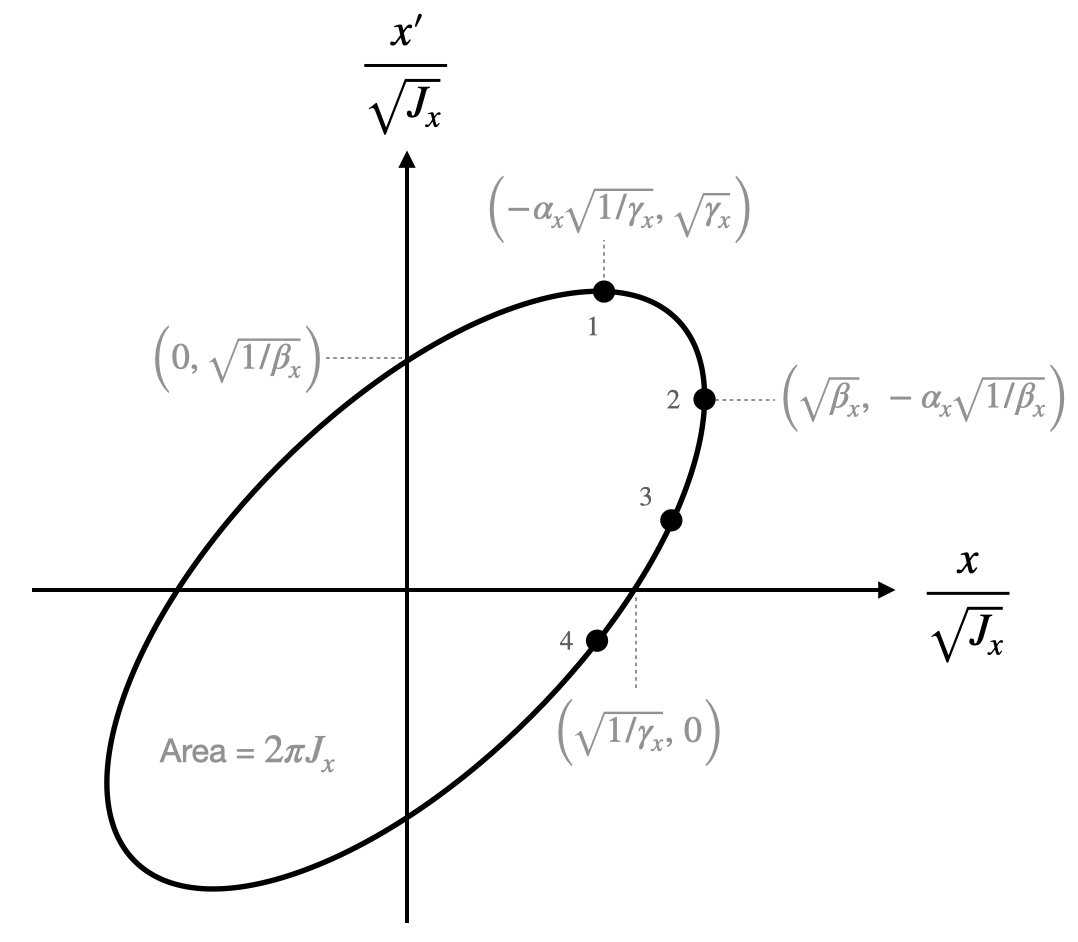
\includegraphics[width=0.6\textwidth]{Images/chapter1/cs_ellipse.png}
    \caption{Courant-Snyder ellipse in horizontal phase space.}
    \label{fig:cs_ellipse}
\end{figure}
%
The particle jumps around the boundary of an ellipse. The so-called Twiss parameters $\beta$, $\alpha = -\beta' / 2$, and $\gamma = (1 + \alpha^2) / \beta$ determine the ellipse dimensions. $J$ is called the Courant-Snyder invariant and is proportional to the area of the ellipse, which is conserved due to Liouville's theorem:
%
\begin{equation}\label{eq:CS invariant}
    J = \frac{x^2 + (\alpha x + \beta x')^2}{\beta}.
\end{equation}
%
We define the tune $\nu$ as the number of phase space oscillations per turn; i.e.,
%
\begin{equation}
    2\pi\nu = \oint{\frac{ds}{\beta(s)}},
\end{equation}
%
where the integral is around the entire ring.

Thus, motion between two locations in the ring is equivalent to an area-preserving linear transformation of a phase space ellipse, plus rotation of the particle around the ellipse. This is more clear in the transfer matrix formulation of the dynamics, writing $\mathbf{x}(s) = \mathbf{M}(s)\mathbf{x}(0)$ where
%
\begin{equation} \label{eq:CS_parameterization}
\begin{aligned}
    \mathbf{M}(s) &= 
    \begin{bmatrix} 
        \sqrt{\beta(s)} & 0 \\
        -\frac{\alpha(s)}{\sqrt{\beta(s)}} & \sqrt{\frac{1}{\beta(s)}}
    \end{bmatrix}
    \begin{bmatrix} 
        \cos\mu(s) & \sin\mu(s) 
        \\ -\sin\mu(s) & \cos\mu(s) 
    \end{bmatrix}
    \begin{bmatrix} 
        \sqrt{\frac{1}{\beta(0)}} & 0 \\
        \frac{\alpha(0)}{\sqrt{\beta(0)}} & \sqrt{\beta(0)}
    \end{bmatrix} \\
    &= \mathbf{V}(s) \, \mathbf{R}(s) \, \mathbf{V}(0)^{-1}. 
\end{aligned}
\end{equation}
%
$\mathbf{V(0)}^{-1}$ transforms the phase space ellipse into a circle while preserving its area, $\mathbf{R(s)}$ rotates the coordinates around the circle according to the phase advance, and $\mathbf{V(s)}$ transforms the circle back into an ellipse \cite{Lee2011}. 

Eq.~\eqref{eq:CS_parameterization} motivates the definition of normalized phase space coordinates $\mathbf{x}_n(s) = \mathbf{V}(s)^{-1} \mathbf{x}(s)$ in which the particle performs simple harmonic oscillations; i.e., rotates in a circle of area $J$ at frequency $2\pi\nu$. 


\subsection{Linear (coupled) dynamics}

In the presence of linear coupling, Eq.~\eqref{eq:Hill} takes the following form:
%
\begin{equation}\label{eq:single_particle_eom_coupled}
\begin{aligned}
    x'' + k_{11}(s)x + k_{13}(s)y + k_{14}(s)y' &= 0, \\
    y'' + k_{33}(s)y + k_{31}(s)x + k_{32}(s)x' &= 0,
\end{aligned}
\end{equation}
%
Liouville's theorem is no longer valid in two-dimensional (2D) phase space; instead, the particle moves along the boundary of an ellipsoid in 4D phase space ($x$-$x'$-$y$-$y'$). For example, Fig.~\ref{fig:skew_quad_single_particle_tbt} shows the turn-by-turn trajectory of a single particle in the presence of linear coupling from a rotated (skew) quadrupole.
%
\begin{figure}[!p]
    \centering
    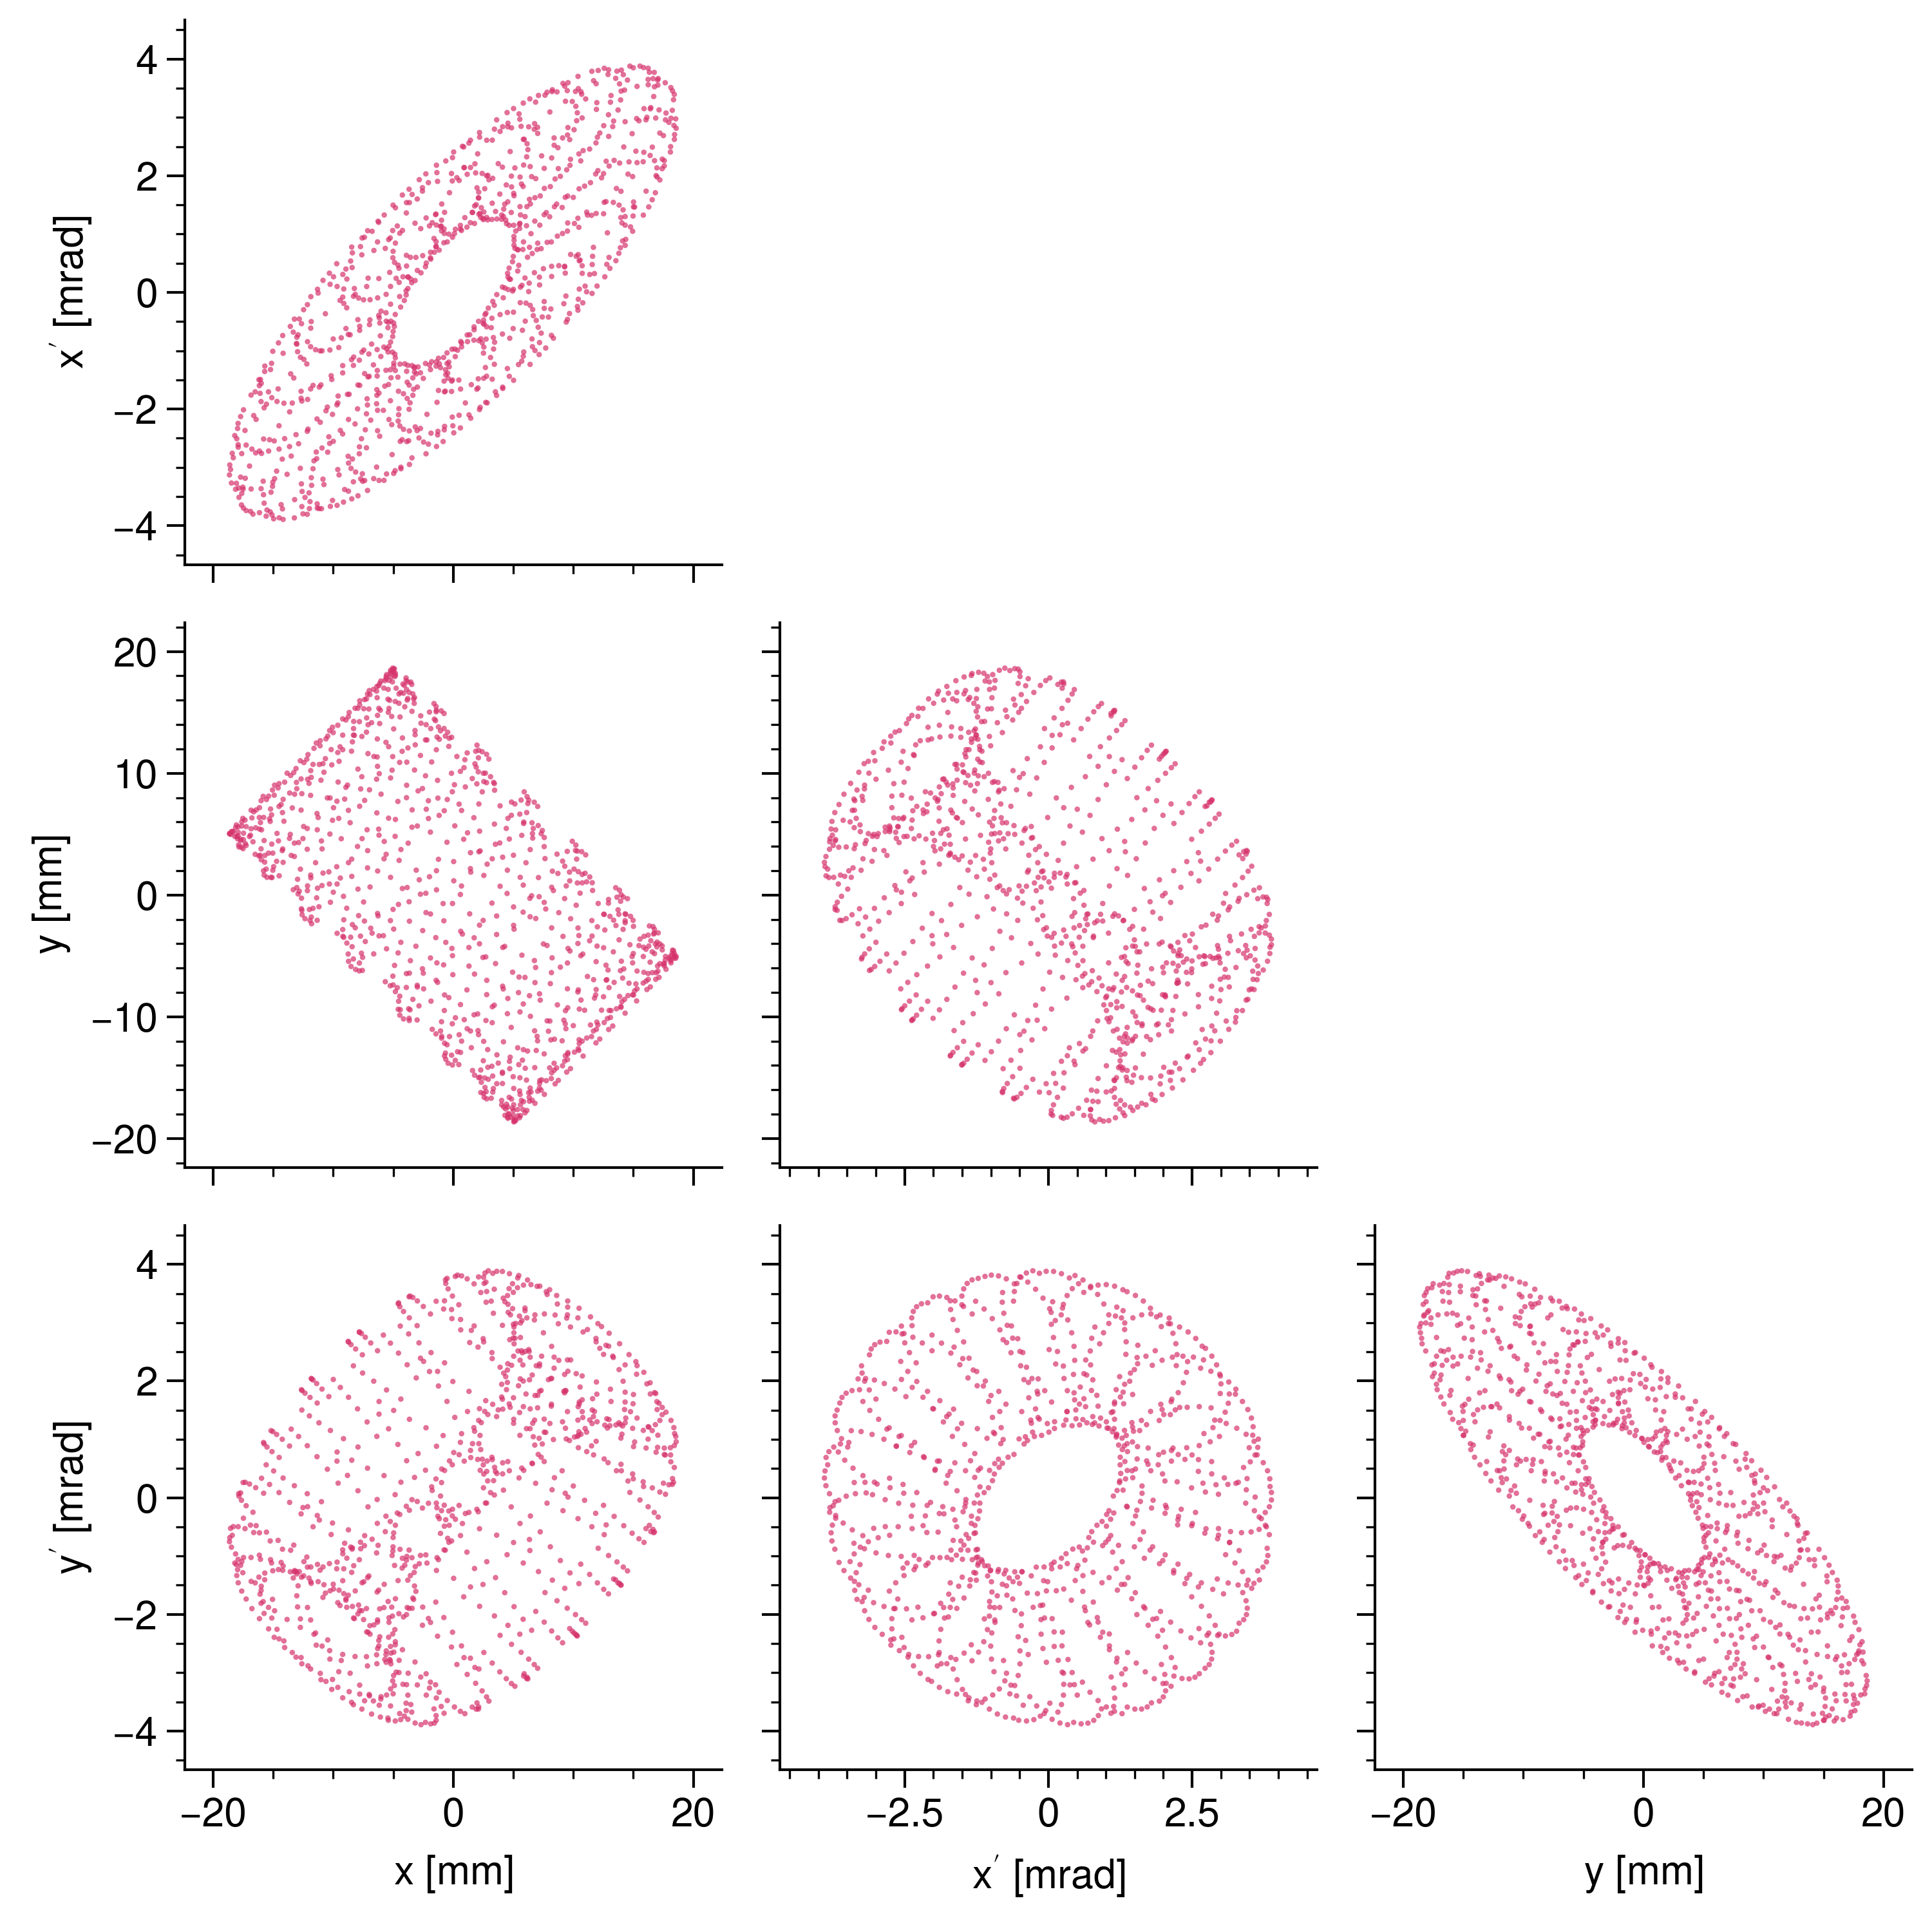
\includegraphics[width=0.85\textwidth]{Images/chapter1/skew_quad_single_particle_tbt.png}
    \caption{Turn-by-turn trajectory of a particle in a linear lattice with the addition of a skew quadrupole.}
    \label{fig:skew_quad_single_particle_tbt}
\end{figure}
%
The motion is most simply described using transfer matrices. Consider the eigenvectors and eigenvalues of the $4 \times 4$ symplectic one-turn transfer matrix $\mathbf{M}$. There are four eigenvectors — $\mathbf{v}_1$, $\mathbf{v}_2$, $\mathbf{v}_1^*$, $\mathbf{v}_2^*$ — and four eigenvalues — $\lambda_1$, $\lambda_2$, $\lambda_1^*$, $\lambda_2^*$ — with $\lambda_1\lambda_2 = 1$ (* denotes the complex conjugate). The eigenvalue equation is written as
%
\begin{equation} \label{eq:transfer_matrix_eig}
    \mathbf{M} \mathbf{v}_l = e^{-i\mu_l} \mathbf{v}_l,
\end{equation}
%
with $l = 1,2$. The phase space coordinate vector $\mathbf{x} = (x, x', y, y')^T$ at one position in the ring is a linear combination of the eigenvectors:
%
\begin{equation}
    \mathbf{x} = Re \left\{
        \sqrt{2 J_1} \, \mathbf{v}_1 \, e^{-i\psi_1}
        + \sqrt{2 J_2} \, \mathbf{v}_2 \, e^{-i\psi_2}
    \right\},
\end{equation}
%
where $J_{1,2}$ are constant amplitudes and $\psi_{1,2}$ are initial phases. Application of the transfer matrix advances the phases:
%
\begin{equation}\label{eq:eigvec_coords}
    \mathbf{Mx} = Re \left\{
        \sqrt{2 J_1} \, \mathbf{v}_1 \, e^{-i(\psi_1 + \mu_1)}
        + \sqrt{2 J_2} \, \mathbf{v}_2 \, e^{-i(\psi_2 + \mu_2)}
    \right\}.
\end{equation}
%
The old invariants $J_{x,y}$ are replaced by $J_{1,2}$ and the phase advances $\mu_{x,y}$ are replaced by $\mu_{1,2}$. A new normalized phase space is defined by rewriting Eq.~\eqref{eq:eigvec_coords} as $\mathbf{x}_n = \mathbf{V}^{-1} \mathbf{x}$ with
%
\begin{equation}\label{eq:V_from_eigvecs}
    \mathbf{V} = 
    \begin{bmatrix}
        Re\{\mathbf{v}_1\}, & -Im\{\mathbf{v}_1\}, & Re\{\mathbf{v}_2\}, & -Im\{\mathbf{v}_2\}
    \end{bmatrix}.
\end{equation}
%
Particles perform simple harmonic oscillations in normalized phase space, moving in circles of area $J_1$ in the $x_n$-$x_n'$ plane and $J_2$ in the $y_n$-$y_n'$ plane.

We would like to parameterize the eigenvectors as in the uncoupled case. There are currently several parameterizations in existence \cite{Edwards1973, Ripken1989, Wolski2006, Lebedev2010, Qin2009}; we will use the parameterization of Lebedev and Bogacz \cite{Lebedev2010}:
%
\begingroup
\renewcommand*{\arraystretch}{1.1}
\begin{equation}
\begin{aligned}
    \mathbf{v}_1 = 
    \begin{bmatrix}
        \sqrt{\beta_{1x}} \\
        -\frac{\alpha_{1x} + i(1-u)}{\sqrt{\beta_{1x}}} \\
        \sqrt{\beta_{1y}}e^{i\nu_1} \\
        -\frac{\alpha_{1y} + iu}{\sqrt{\beta_{1y}}} e^{i\nu_1} \\
    \end{bmatrix} ,\quad
    \mathbf{v}_2 = 
    \begin{bmatrix}
        \sqrt{\beta_{2x}}e^{i\nu_2} \\
        -\frac{\alpha_{2x} + iu}{\sqrt{\beta_{2x}}}e^{i\nu_2} \\
        \sqrt{\beta_{2y}} \\
        -\frac{\alpha_{2y} + i(1-u)}{\sqrt{\beta_{2y}}} \\
    \end{bmatrix}.
\end{aligned}
\end{equation}
\endgroup
%
The meaning of the new parameters is illustrated in Fig.~\ref{fig:twiss4D}.
%
\begin{figure}[!p]
    \centering
    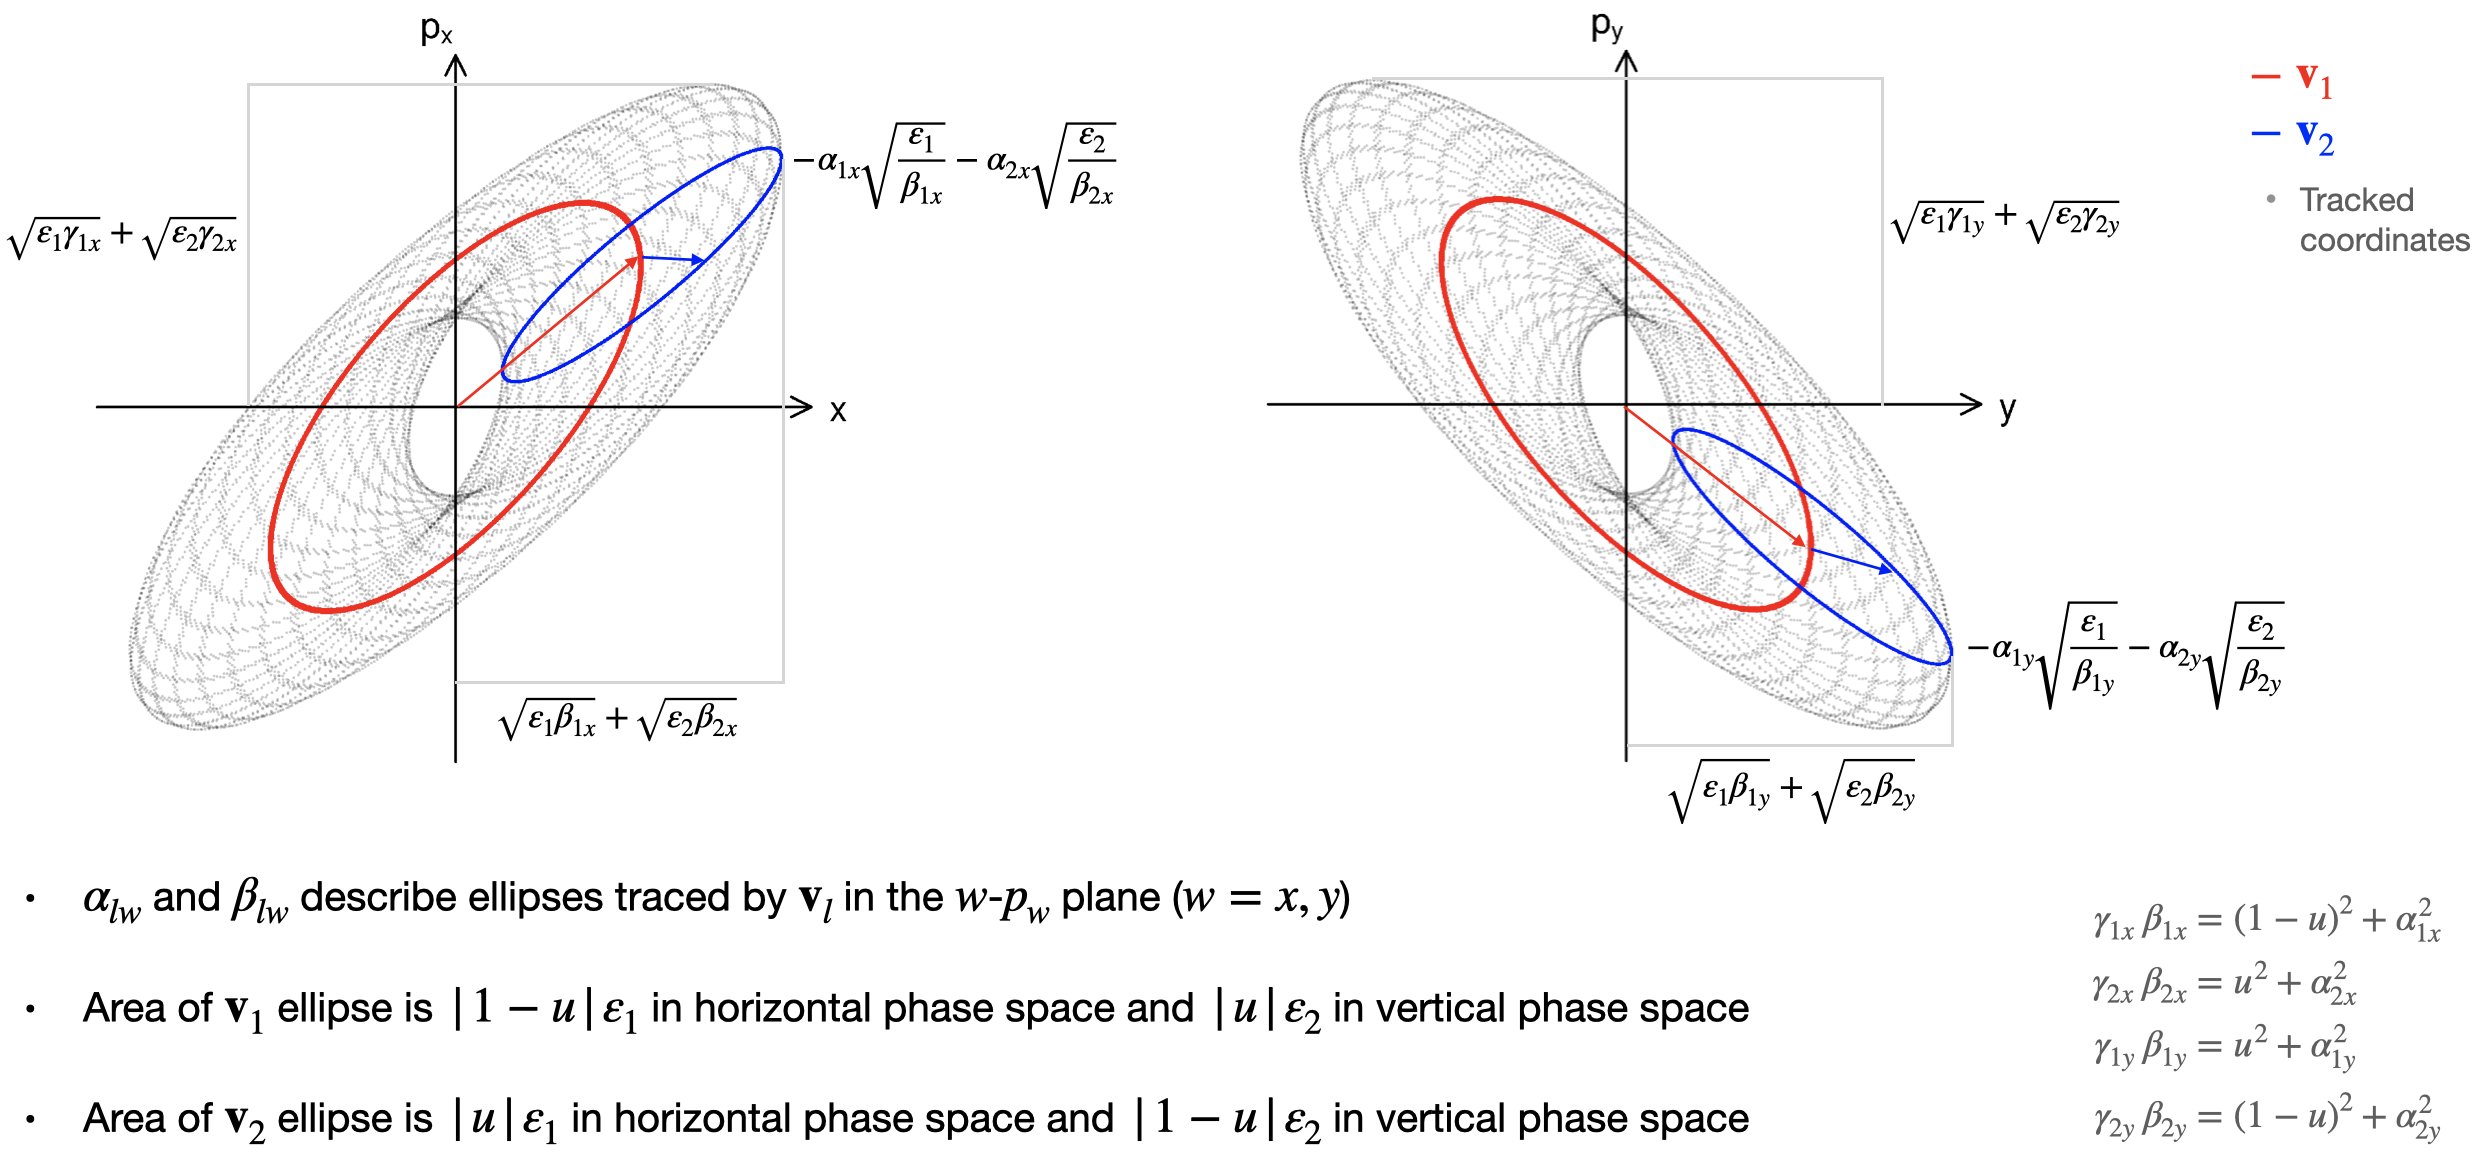
\includegraphics[width=\textwidth]{Images/chapter1/twiss4D.png}
    \vspace*{0.1cm}
    \caption{Lebedev-Bogacz parameterization of coupled motion. The grey markers are the turn-by-turn trajectory of a single particle. The red and blue lines are the ellipses traced by the transfer matrix eigenvectors.}
    \label{fig:twiss4D}
\end{figure}
%
The motion is simply the sum of two eigenvectors, each of which traces an ellipse when projected onto any 2D subspace. The frequency with which the ellipse is traced differs between the two modes; as a consequence, the horizontal and vertical amplitudes $J_x$ and $J_y$ are exchanged. The parameterization assigns a $\beta$ and $\alpha$ parameter to each ellipse. The parameters $\nu_1$ and $\nu_2$ are the phase differences between the horizontal ($x$-$x'$) and vertical ($y$-$y'$) parts of the eigenvectors, which determines the tilt angle of the ellipses traced in the cross-plane projections ($x$-$y$, $x$-$y'$, $y$-$x'$, $x'$-$y'$). Finally, $u$ determines the area of the ellipse traced by the eigenvectors in horizontal phase space relative to the ellipse in vertical phase space. 


\subsection{Nonlinear resonances}

Nonlinear terms in Eq.~\eqref{eq:magnetic_field_expansion} are generally small but nonzero in reality. Following \cite{LundLecture1}, we return to one-dimensional motion and write
%
\begin{equation}\label{eq:Hill_nonlinear}
    x'' + k(s) x = \Delta B,
\end{equation}
%
where $\Delta B$ represents all the nonlinear terms in the expansion (and also linear deviations from the design fields). The stable solution $x_0$ when $\Delta B = 0$ is given by Eq.~\eqref{eq:Hill_solution}. We now define
%
\begin{equation}
    \phi(s) = \frac{1}{\nu} \oint{\frac{ds}{\beta(s)}},
\end{equation}
%
where $\nu$ is the tune. Moving to the normalized coordinate $u = x / \sqrt{\beta}$, with $\dot{u} = du/d\phi$ we have
%
\begin{equation}\label{eq:pert1}
    \ddot{u} + \nu^2 u = -\nu^2 \sum_{n=0}^{\infty}{\left(\beta^{\frac{n+3}{2}} b_{n+1}\right) u^n}.
\end{equation}
%
$\beta$ (the oscillation amplitude of the unperturbed motion) and $b_n$ (a multipole coefficient) are periodic in $\phi$ since they depend only on the position in the ring. Grouping these terms and Fourier expanding gives
%
\begin{equation}
    \ddot{u} + \nu^2 u = -\nu^2 \sum_{n=0}^{\infty}\sum_{k=-\infty}^{\infty} C_{n,k} \, u^n \, e^{ik\phi}.
\end{equation} 
%
We then perturb around $u_0$, the solution to the homogeneous equation, writing $u = u_0 + \delta u$, and keep only linear powers of $\delta u$. 
%
\begin{equation}
    \ddot{\delta u} + \nu^2 \delta u \approx -\nu^2 \sum_{n=0}^{\infty}\sum_{k=-\infty}^{\infty} C_{n,k} \, u_0^n \, e^{ik\phi}.
\end{equation}
%
Noting that
%
\begin{equation}
    u_0^n \propto \cos^n(\nu\phi) = \frac{1}{2^n}\sum_{m=0}^{n} \binom{n}{m} e^{i(n-2m)\nu\phi},
\end{equation} 
%
leads to
%
\begin{equation}\label{eq:pert2}
    \ddot{\delta u} + \nu^2 \delta u \approx -\nu^2 \sum_{n=0}^{\infty}\sum_{k=-\infty}^{\infty} \sum_{m=0}^{n} {n \choose m} \frac{C_{n,k}}{2^n} e^{i\left[(n - 2m)\nu + k\right]\phi}.
\end{equation}
%
A resonance condition may occur when any of the frequency components of the driving terms are close to the tune $\nu$; i.e., when
%
\begin{equation}
    (n - 2m)\nu + k = \pm \nu.
\end{equation}
%
Dipole terms correspond to integer tunes, quadrupole terms to 1/2 integer tunes, sextupole terms to 1/3 integer tunes, and so on. The same is true in the vertical dimension. The inclusion of coupling between $x$ and $y$ leads to the following resonance conditions:
%
\begin{equation}\label{eq:resonance_lines}
    M_x \nu_x + M_y \nu_y = N,
\end{equation}
%
where $M_x$, $M_y$, and $N$ are integers and $|M_x| + |M_y|$ is the order of the resonance. These resonance lines are plotted in Fig.~\ref{fig:resonance_lines}.
%
\begin{figure}[!p]
    \centering
    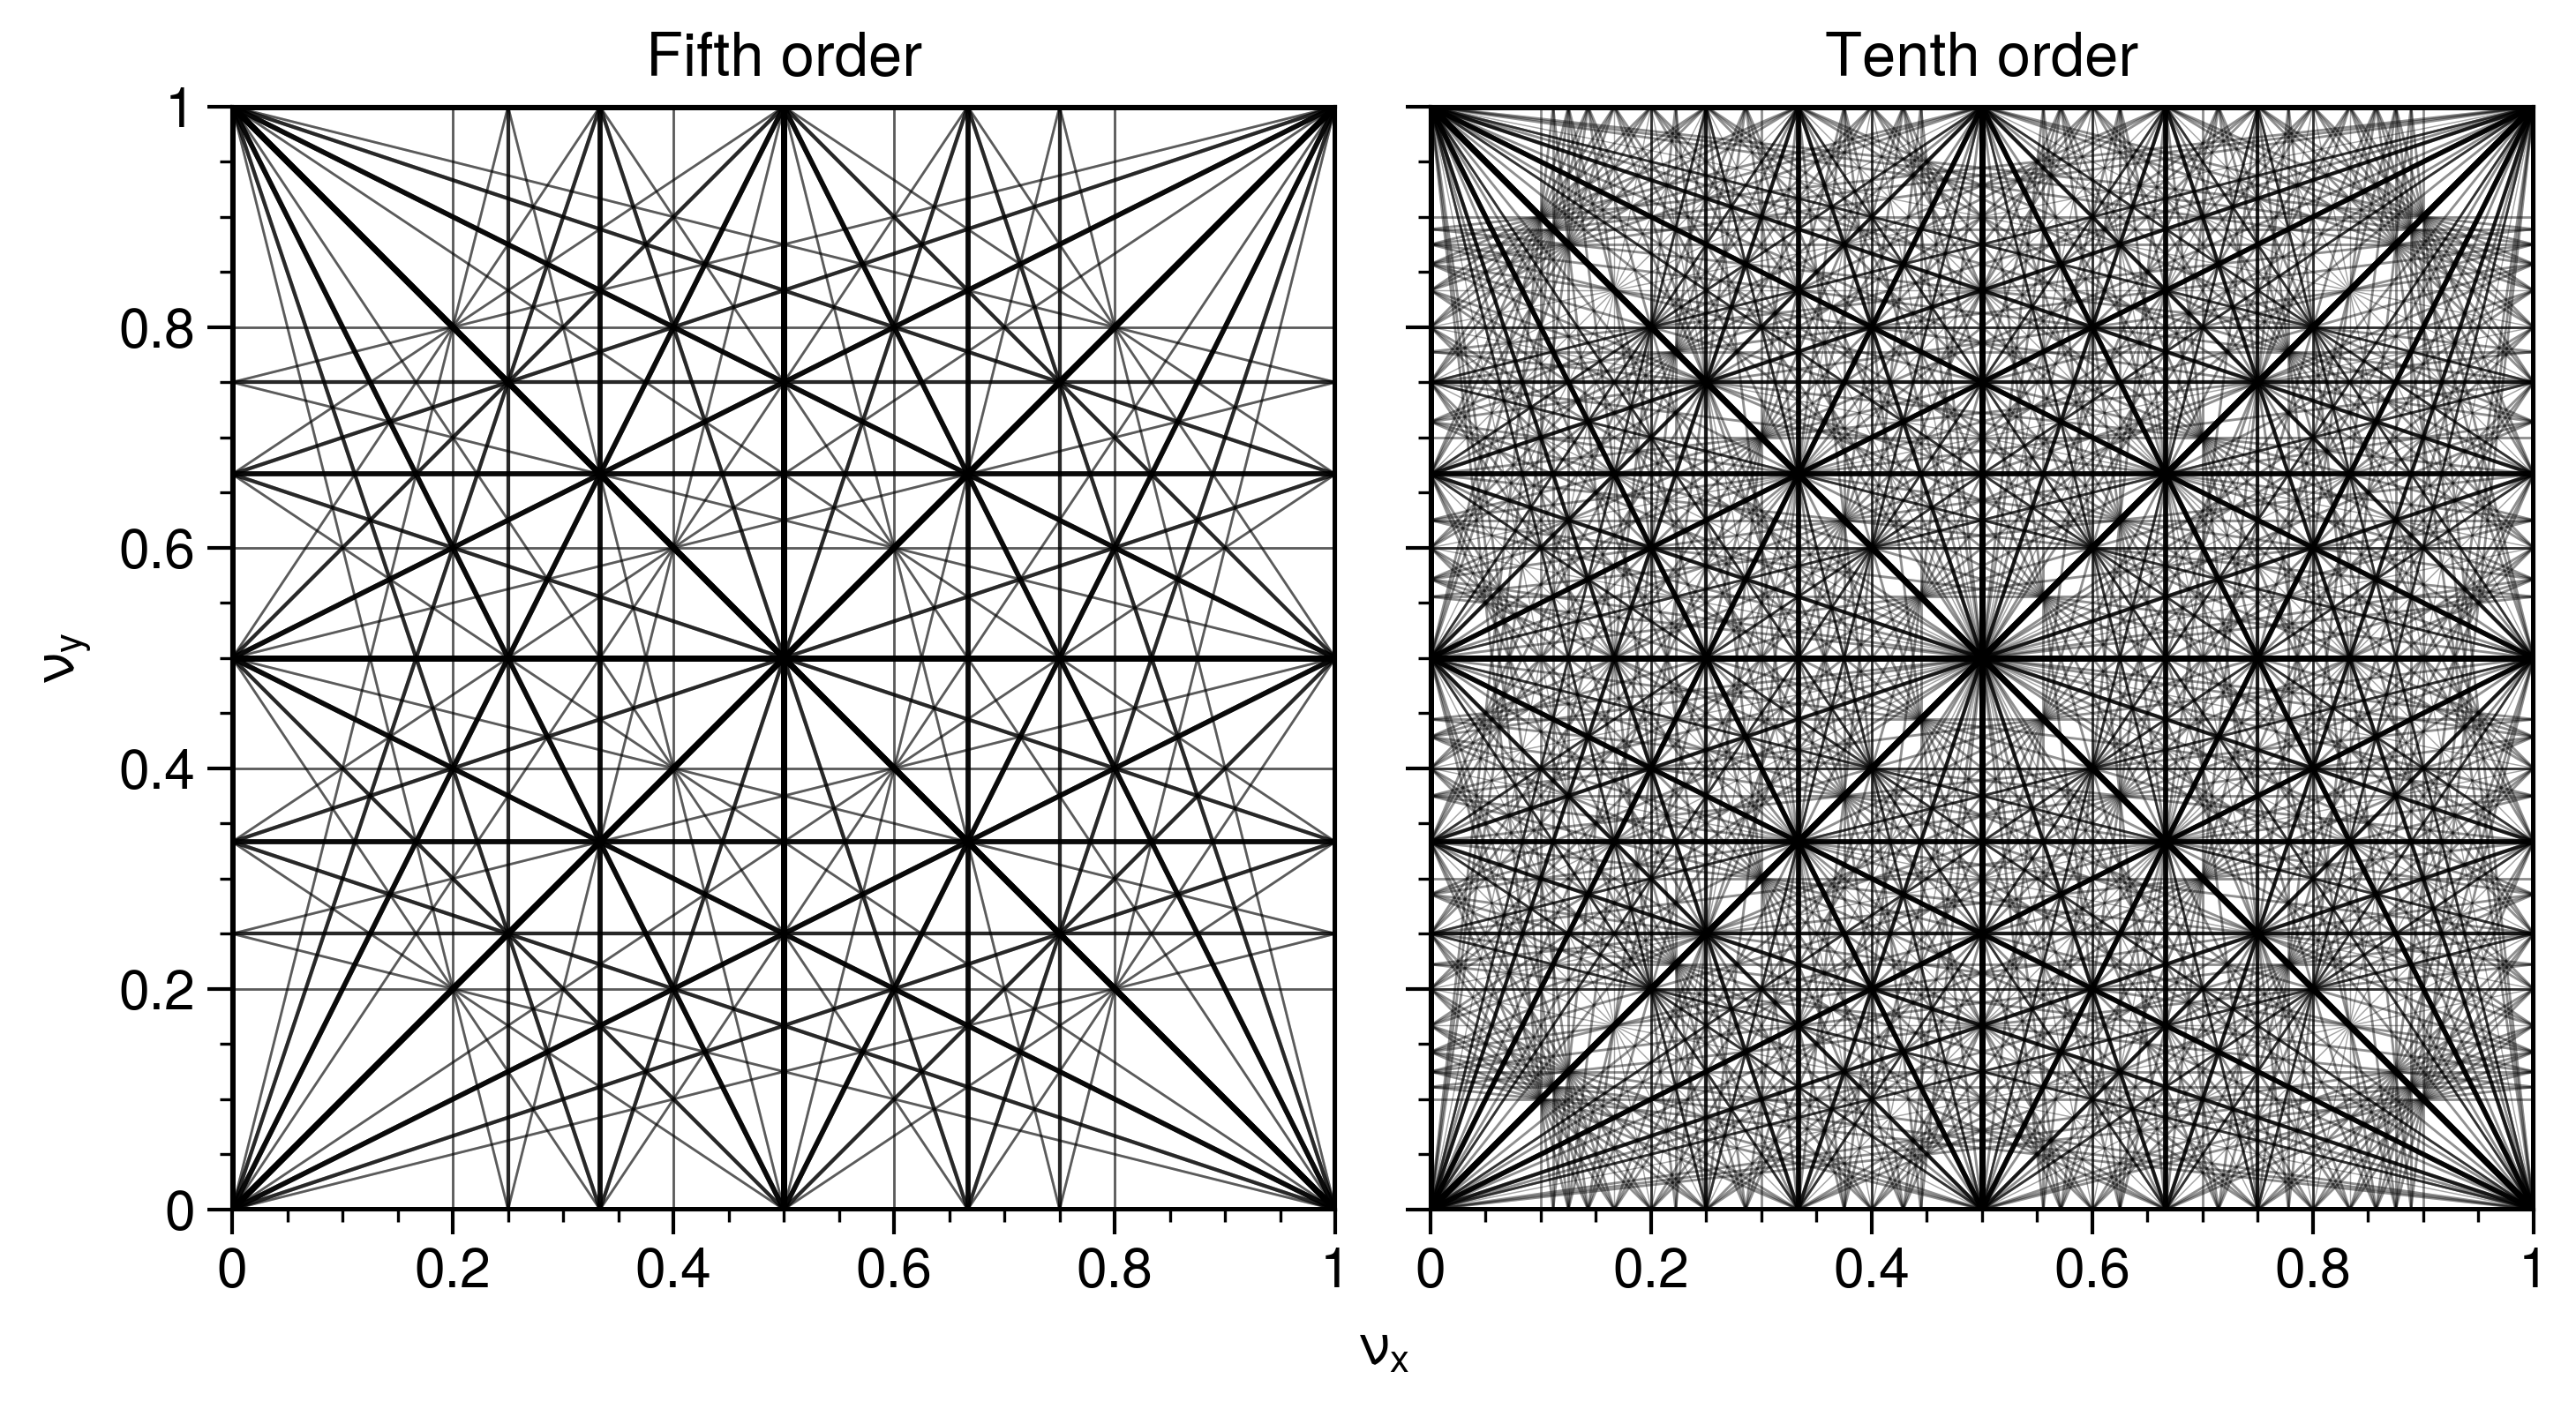
\includegraphics[width=\textwidth]{Images/chapter1/resonance_lines.png}
    \caption{Resonance lines in tune space defined by Eq.~\eqref{eq:resonance_lines}.}
    \label{fig:resonance_lines}
\end{figure}
%
\begin{figure}[!p]
    \begin{subfigure}[b]{1.0\textwidth}
        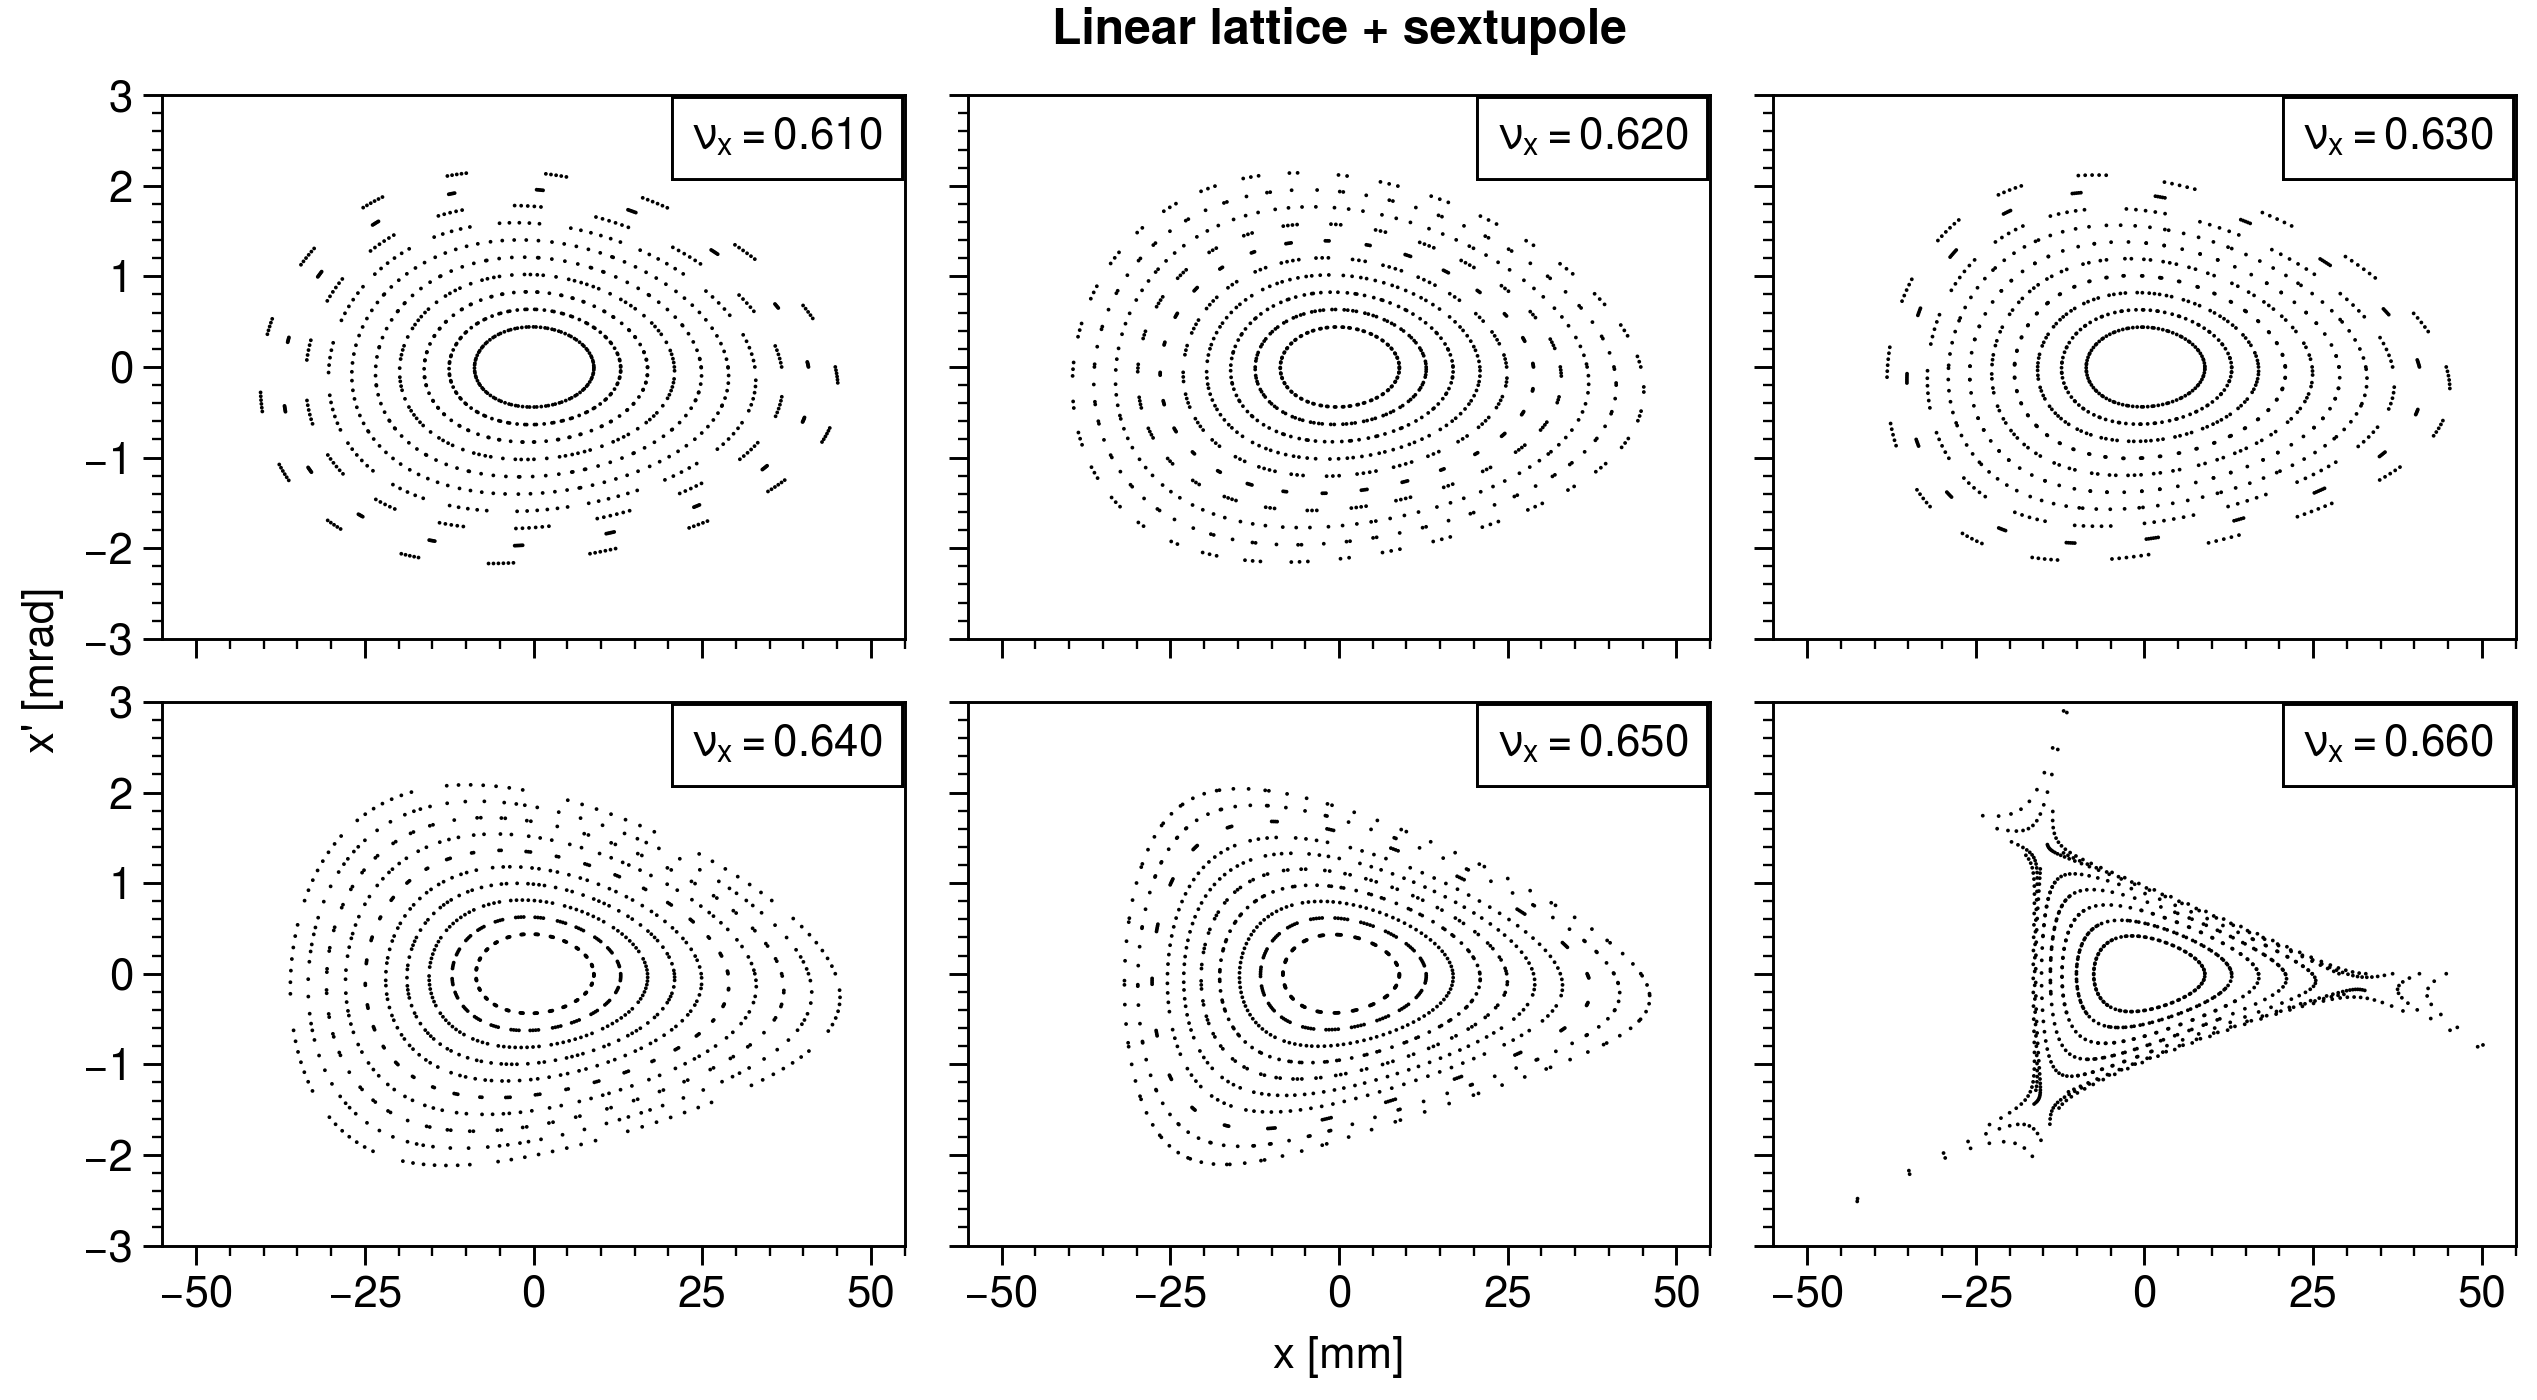
\includegraphics[width=\textwidth]{Images/chapter1/sextupole.png}
        \label{fig:sextupole_a}
    \end{subfigure}
    \vfill
    \vspace*{1.0cm}
    \vfill
    \begin{subfigure}[b]{\textwidth}
        \centering
        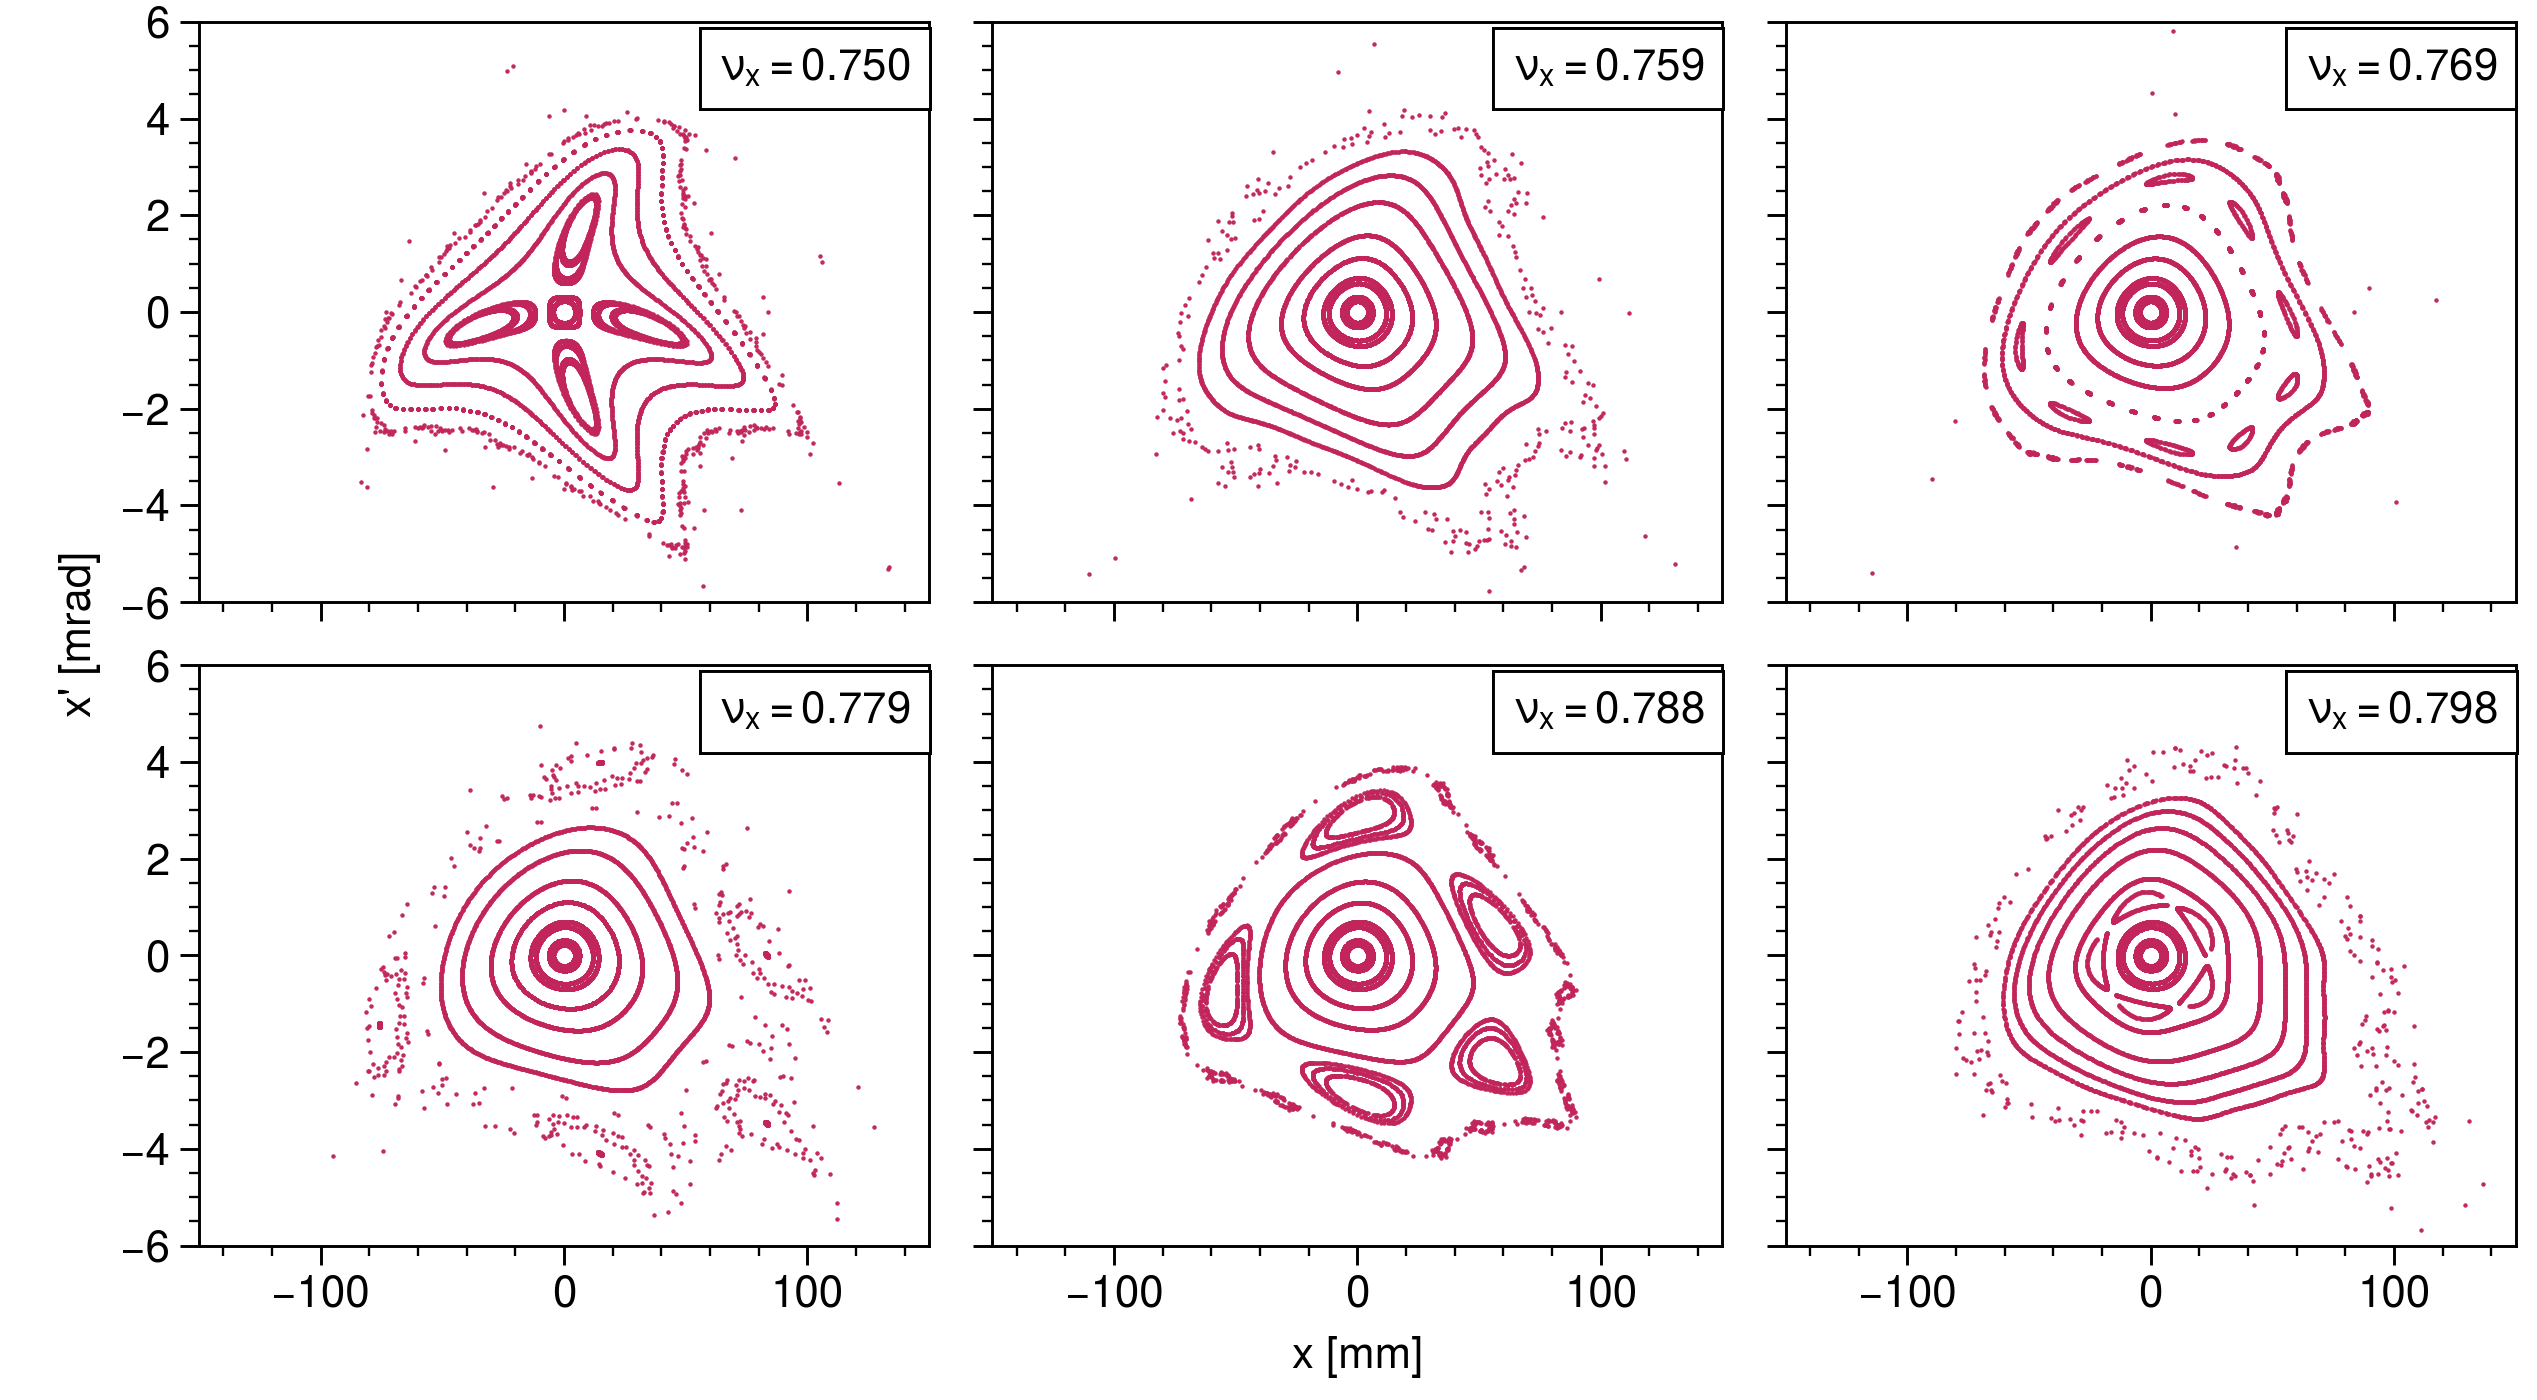
\includegraphics[width=\textwidth]{Images/chapter1/sextupole_second_order.png}
        \label{fig:sextupole_b}
    \end{subfigure}
    \caption{Third-order (top) and fourth/fifth-order (bottom) resonances excited by a sextupole perturbation to a linear lattice. (Adapted from \cite{Lee2011}.)}
    \label{fig:sextupole}
\end{figure}
%
The strength of the resonance varies inversely with the order; fourth-order and below are the primary concern in most machines, but higher-order effects may be important when the number of stored turns is large. 

Nonlinear resonances can be studied quickly using mapping equations \cite{Reichl1992}. For illustration, Fig.~\ref{fig:sextupole} shows two numerical experiments from \cite{Lee2011} involving a sextupole perturbation to an otherwise linear lattice. The turn-by-turn trajectories of particles with several different initial amplitudes are plotted for different tunes $\nu_x$. The third-order resonance leads to a well-known triangular region of stability as the tune approaches 2/3. The bottom plot reveals fourth and fifth-order resonances only obtained from second-order perturbation analysis.


\section{Collective beam description}

A beam is a distribution of particles in phase space. In the limit of many particles, we define a distribution function $f(\mathbf{x})$ such that $f(\mathbf{x}) d\mathbf{x}$ gives the number of particles in an infinitesimal volume of phase space $d\mathbf{x}$. The measurable quantities are generally the projections of the distribution; e.g.
%
\begin{equation}
    f(x) = \int_{-\infty}^{\infty}\int_{-\infty}^{\infty}\int_{-\infty}^{\infty} f(x, x', y, y') dx' dy dy'.
\end{equation}
%

It is often sufficient to characterize a distribution by its covariance matrix {$\bm{\Sigma} = \langle{\mathbf{x}\mathbf{x}^T}\rangle$}, where $\langle{\dots}\rangle$ represents the average over the distribution. In the transverse plane:
%
\begin{equation}\label{eq:covariance_matrix}
\begin{aligned}
    \bm{\Sigma} &= 
    \begin{bmatrix}
        \langle{xx}\rangle & \langle{xx'}\rangle & \langle{xy}\rangle & \langle{xy'}\rangle \\
        \langle{xx'}\rangle & \langle{x'x'}\rangle & \langle{x'y}\rangle & \langle{x'y'}\rangle \\
        \langle{xy}\rangle & \langle{x'y}\rangle & \langle{yy}\rangle & \langle{yy'}\rangle \\
        \langle{xy'}\rangle & \langle{x'y'}\rangle & \langle{yy'}\rangle & \langle{y'y'}\rangle 
    \end{bmatrix}
    &= 
    \begin{bmatrix}
        \bm{\sigma}_{xx} & \bm{\sigma}_{xy} \\
        \bm{\sigma}^T_{xy} & \bm{\sigma}_{yy}
    \end{bmatrix}.
\end{aligned}
\end{equation}
%
If a linear transformation $\mathbf{x} \rightarrow \mathbf{M}\mathbf{x}$ is applied to the coordinates, the covariance matrix transforms as
%
\begin{equation}\label{covariance_matrix_transport}
    \bm{\Sigma} 
    \rightarrow 
    \mathbf{M} \, \bm{\Sigma} \, \mathbf{M}^T.
\end{equation}
%
The covariance matrix defines an ellipsoid in phase space. The 4D emittance $\varepsilon_{4D}$ is proportional to the volume of this ellipsoid:
%
\begin{equation} 
    \varepsilon_{4D} = \left|{\Sigma}\right|^{1/2}
\end{equation}
%
where $|...|$ is the determinant. The 4D emittance is conserved under any linear transformation. The horizontal and vertical emittances $\varepsilon_{x,y}$ are individually conserved if the transformation is uncoupled:
%
\begin{equation}
\begin{aligned}
    \varepsilon_x &= \left|{\bm\sigma}_{xx}\right|^{1/2}, \\
    \varepsilon_y &= \left|{\bm\sigma}_{yy}\right|^{1/2}
\end{aligned}
\end{equation}
%
These correspond to the areas in the $x$-$x'$ and $y$-$y'$ planes. In the absence of cross-plane correlations ($\bm{\sigma}_{xy} = 0$), the 4D emittance is equal to the product of the horizontal and vertical emittances.

It is challenging to generate initial distributions for simulations \cite{Lund2009}. For simple applications, a common strategy is to assume elliptical symmetry and construct a distribution from the single-particle invariants $J_{x,y}$. We define the ellipsoid parameter $T$ as 
%
\begin{equation}
    T = \frac{J_x}{\varepsilon_x} + \frac{J_y}{\varepsilon_y}
\end{equation}
%
and stack ellipsoids to create the distribution, writing $f = f(T)$. One option is a Gaussian distribution. In normalized coordinates:
%
\begin{equation}
    f_{gauss} \propto \exp(-T/2).
\end{equation}
%
Another is the Waterbag distribution, which is a uniformly filled ellipsoid:
%
\begin{equation}
    f_{wb} \propto \Theta(1 - T),
\end{equation}
%
where $\Theta$ is the Heaviside step function. Another is the KV distribution, which is a uniformly populated ellipsoidal shell:
%
\begin{equation}
    f_{kv} \propto \delta(1 - T)
\end{equation}
%
The 1D and 2D projections of these 4D distributions are shown in Fig.~\ref{fig:distributions_gaussian}, Fig.~\ref{fig:distributions_waterbag}, and Fig.~\ref{fig:distributions_kv}. The black ellipse shows the covariance matrix ellipsoid projected onto the planes, multiplied by a factor of four. Since the distributions share the same covariance matrix, they are said to be rms-equivalent.
%
\begin{figure}[!p]
    \begin{subfigure}{0.49\textwidth}
        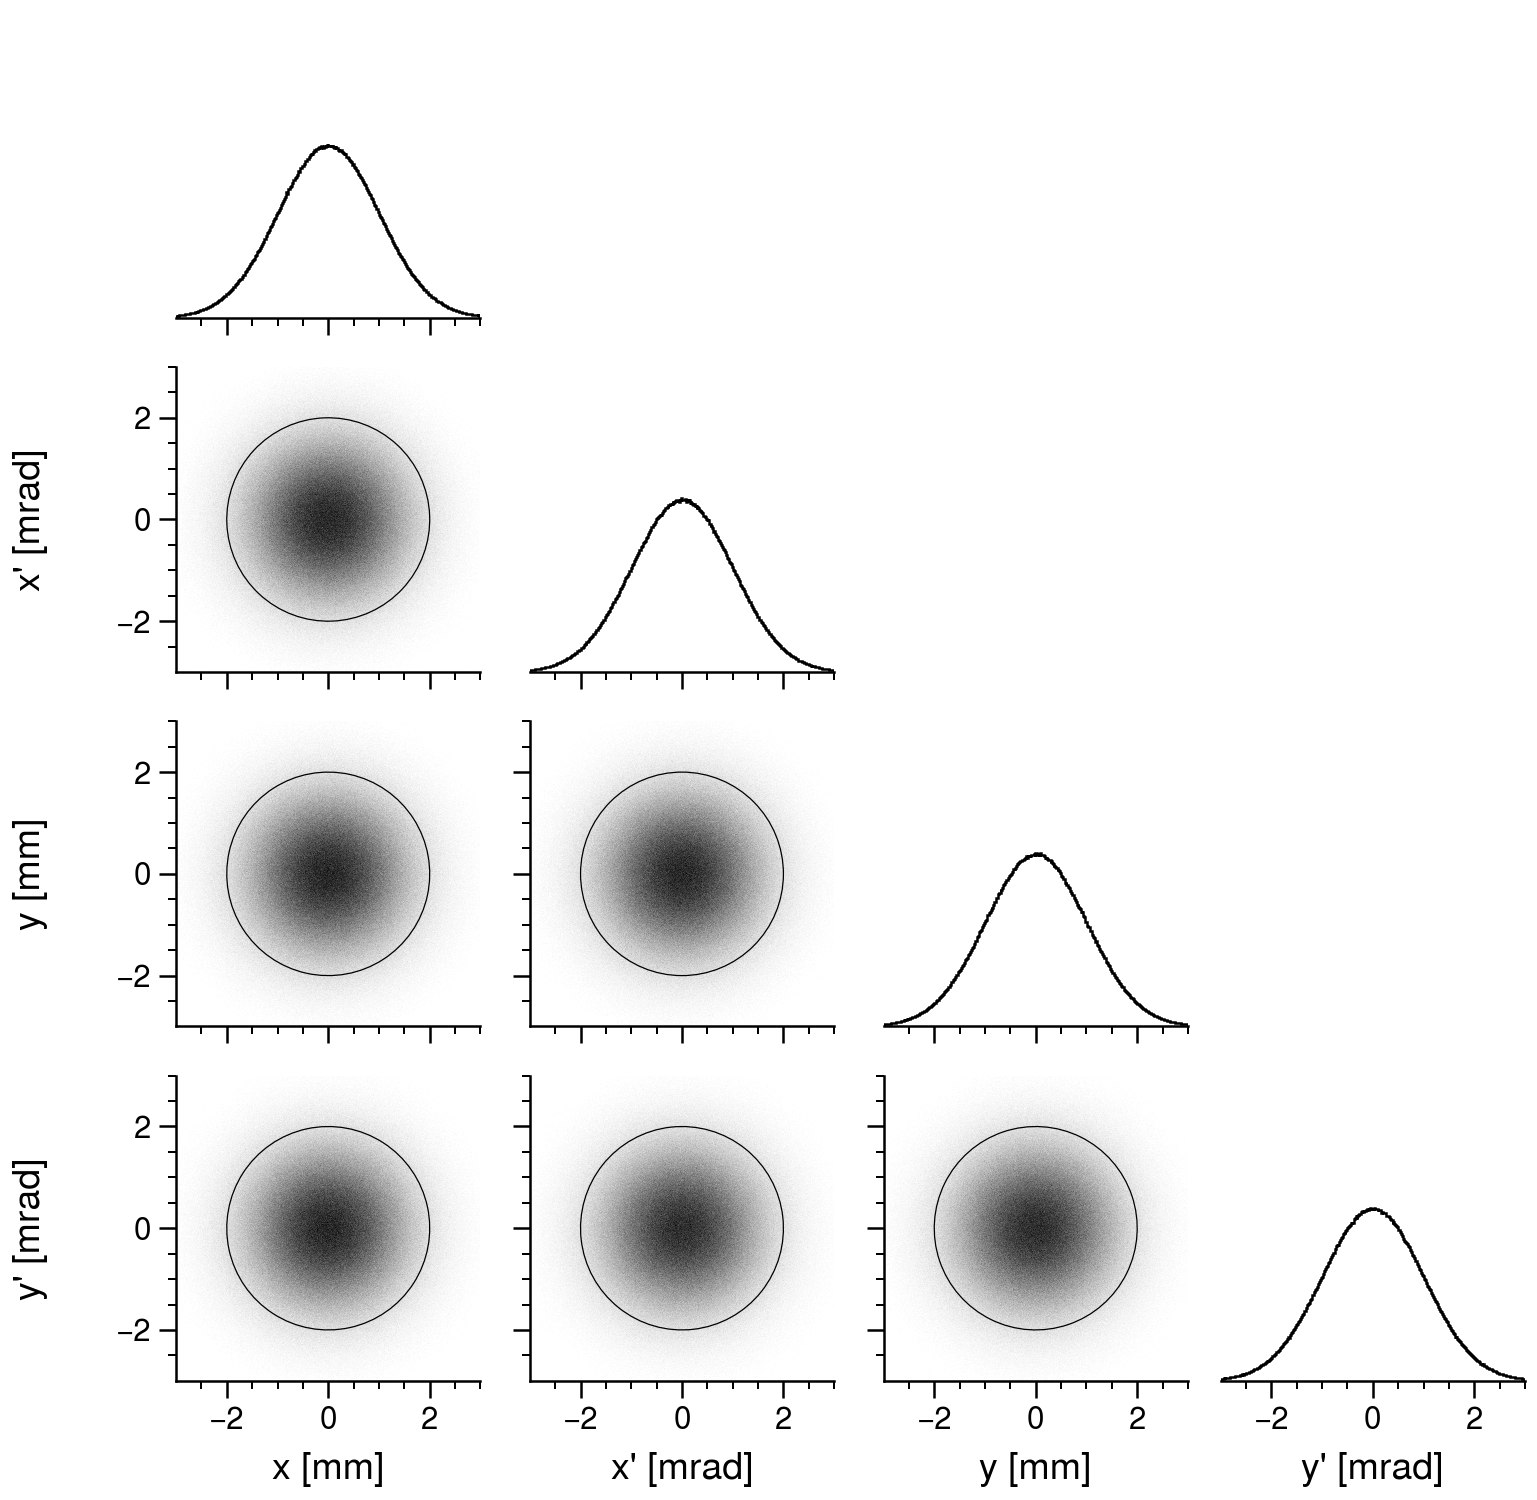
\includegraphics[width=\textwidth]{Images/chapter1/Gaussian_dist.png}
        \caption{Gaussian distribution}
        \label{fig:distributions_gaussian}
    \end{subfigure}
    \hfill
    \begin{subfigure}{0.49\textwidth}
        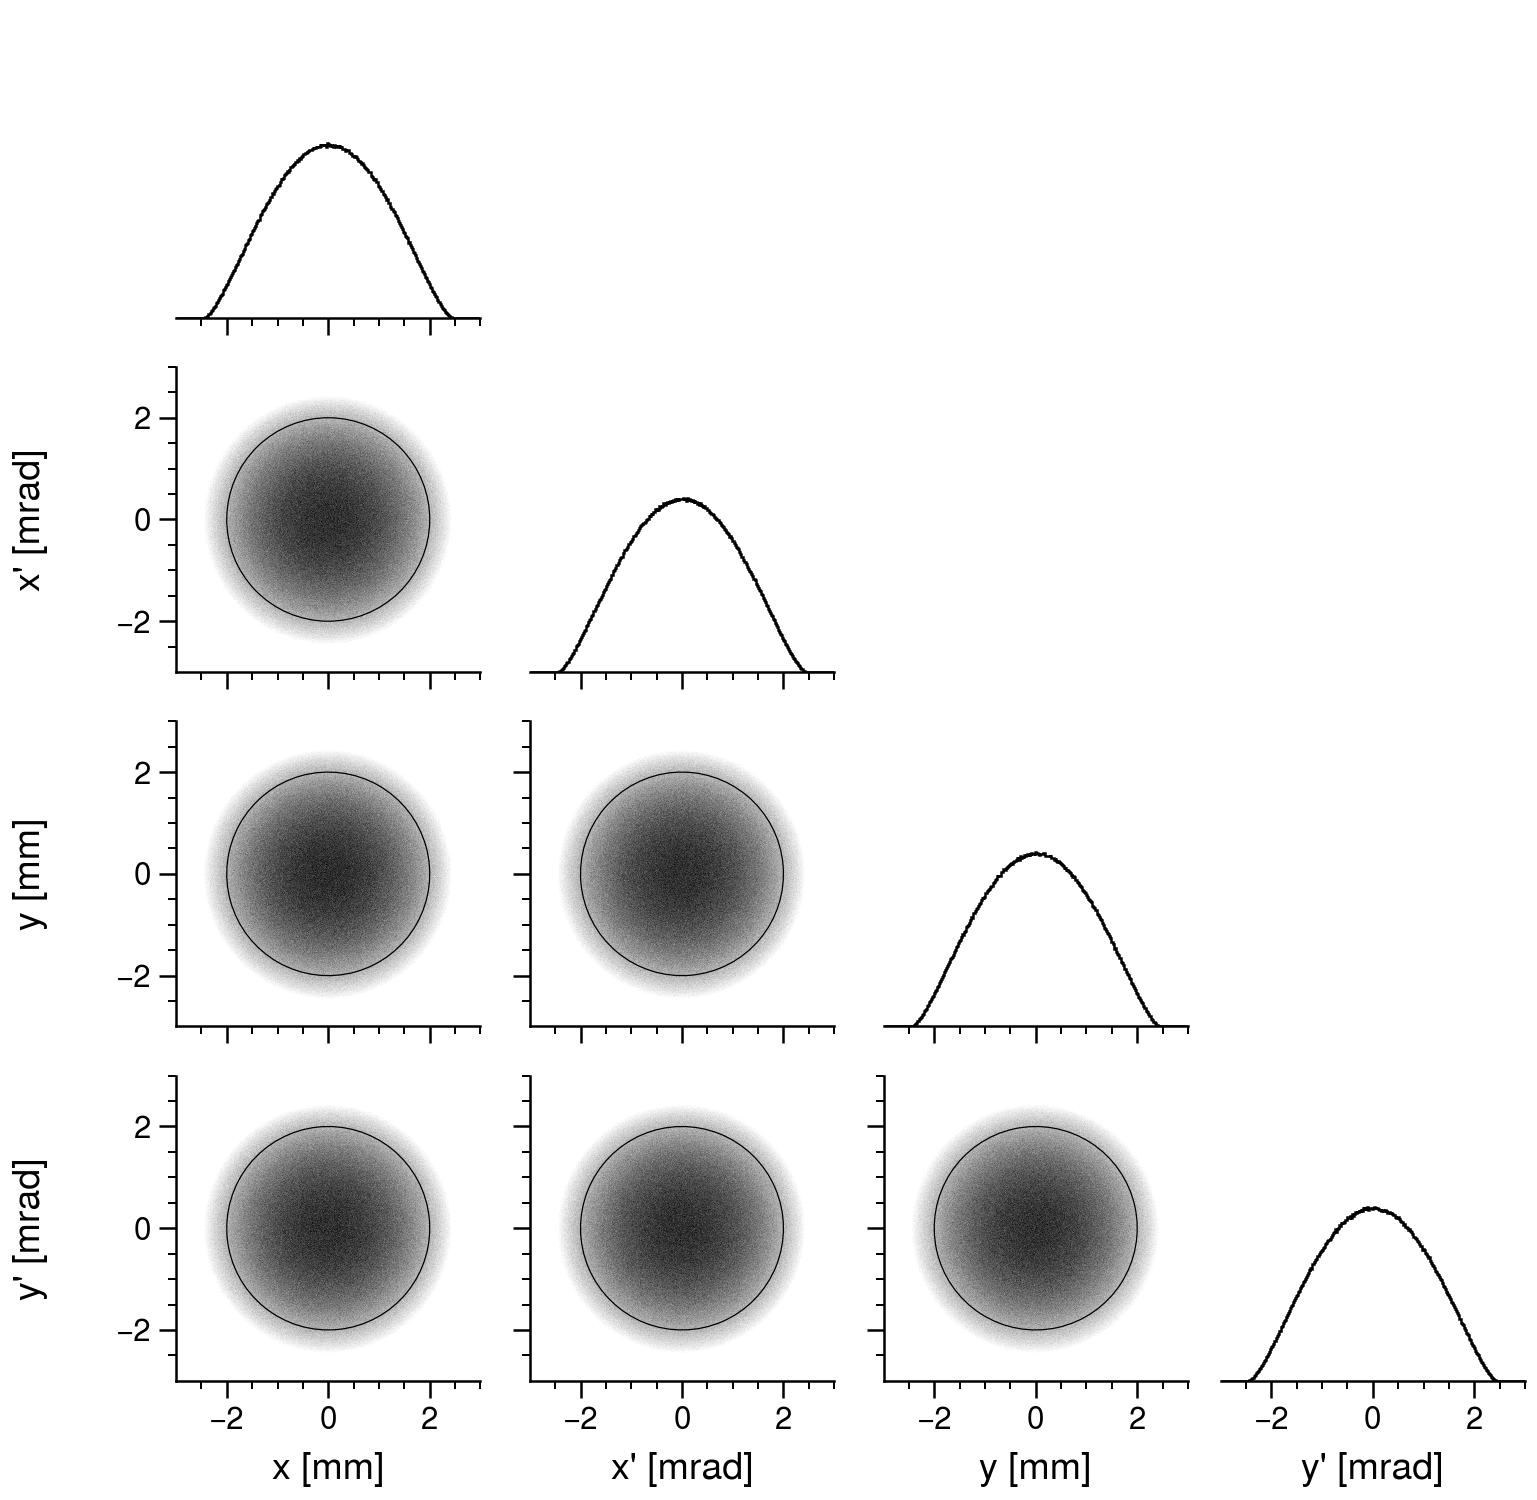
\includegraphics[width=\textwidth]{Images/chapter1/Waterbag_dist.png}
        \caption{Waterbag distribution}
        \label{fig:distributions_waterbag}
    \end{subfigure}
    \vfill
    \begin{subfigure}{0.49\textwidth}
        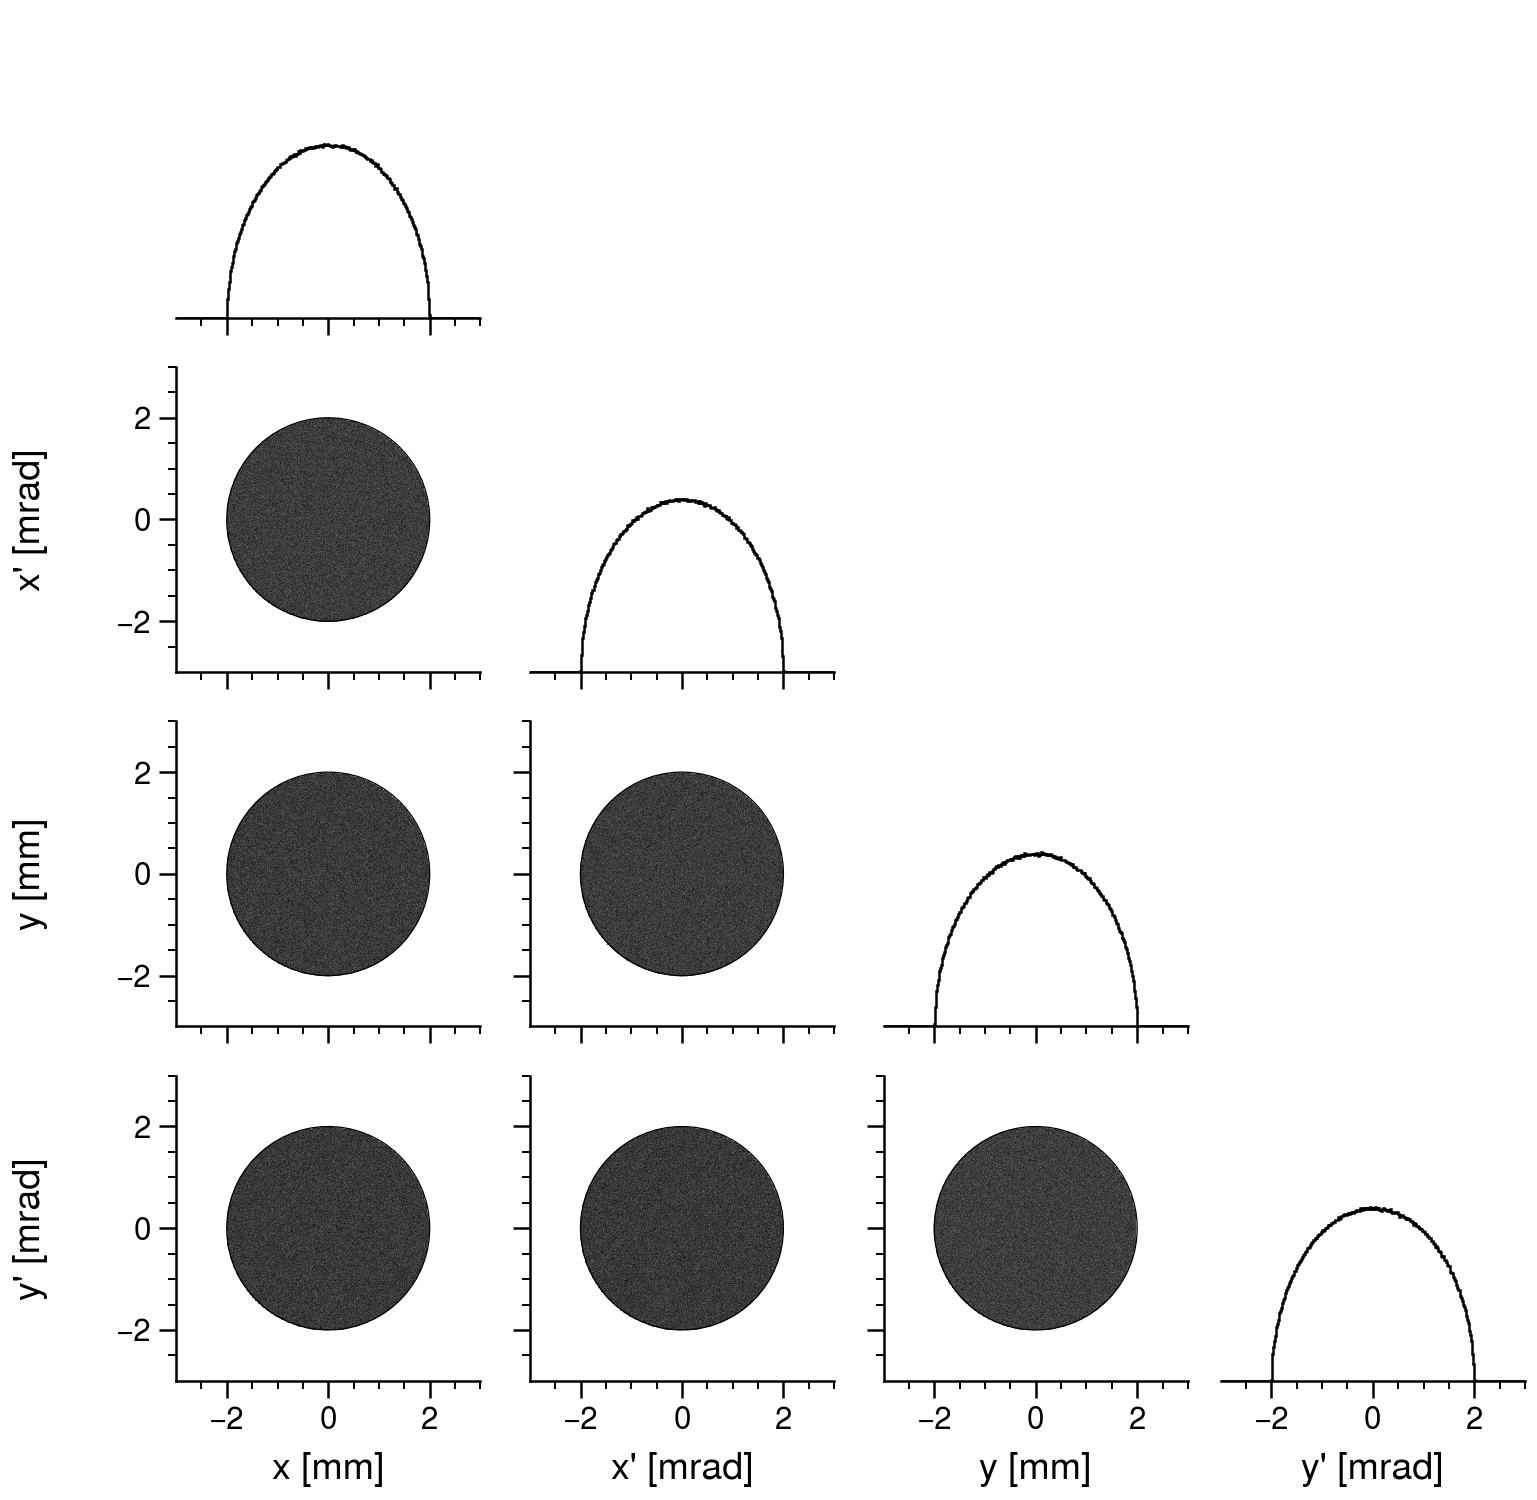
\includegraphics[width=\textwidth]{Images/chapter1/KV_dist.png}
        \caption{KV distribution}
        \label{fig:distributions_kv}
    \end{subfigure}
    \hfill
    \begin{subfigure}{0.49\textwidth}
        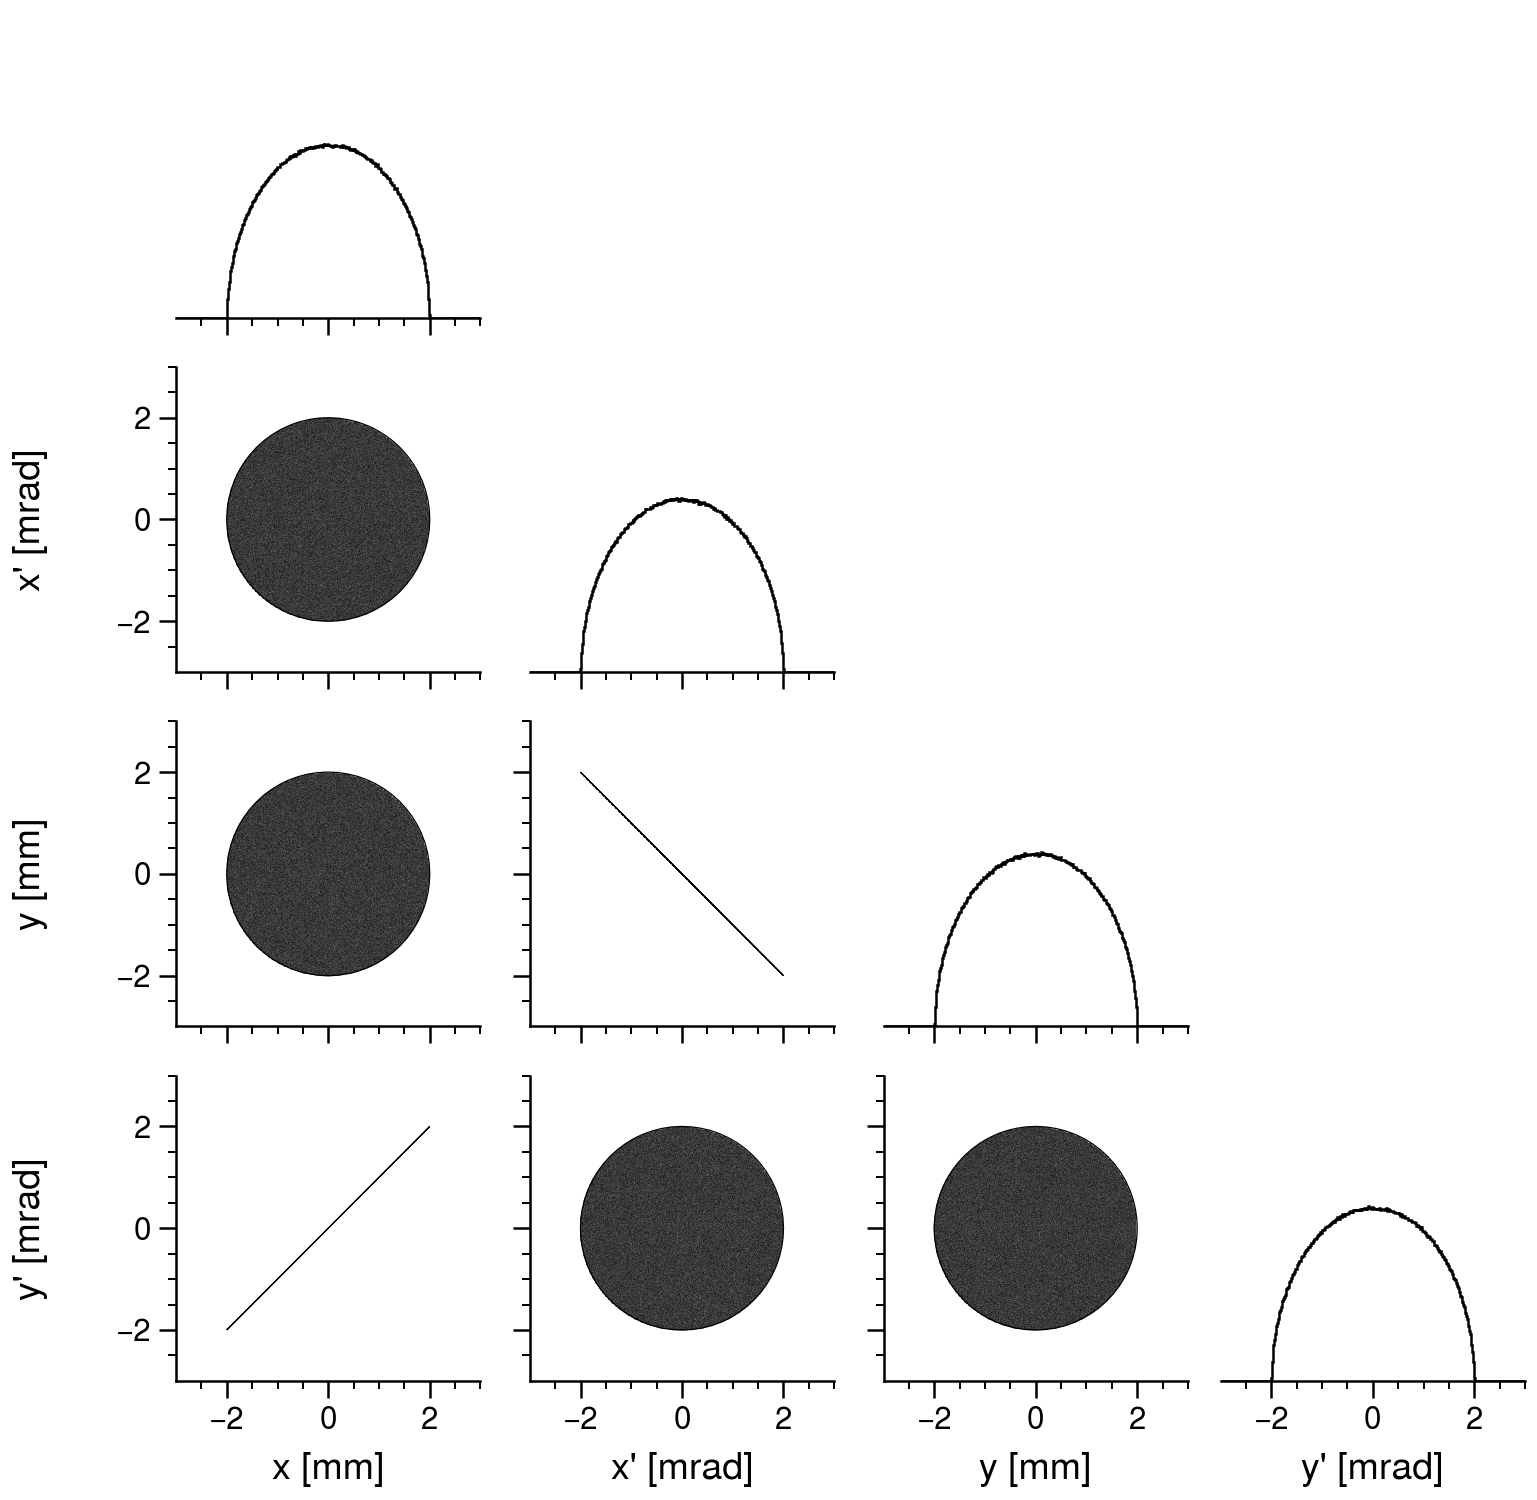
\includegraphics[width=\textwidth]{Images/chapter1/Danilov_dist.png}
        \caption{Danilov distribution}
        \label{fig:distributions_danilov}
    \end{subfigure}
    \caption{1D and 2D projections of various 4D phase space distributions. Black ellipses are defined by four times the distribution covariance matrix.}
    \label{fig:distributions}
\end{figure}
%





\section{Space charge}\label{sec:Space charge}

Particle motion is also influenced by the beam space charge — the charge density of the beam in free space. The beam electric field $\mathbf{E} = (E_x, E_y)$ modifies the single-particle equation of motion:
%
\begin{equation} \label{eq:eom_with_spacecharge}
\begin{aligned}
    x'' + k_x(s)x &= \frac{q}{m \gamma^3 \beta^2 c^2} E_x, \\
    y'' + k_y(s)y &= \frac{q}{m \gamma^3 \beta^2 c^2} E_y,
\end{aligned}
\end{equation}
%
where $\gamma = \left( 1 - \beta^2 \right)^{-1/2}$. The Lorentz factors in the denominator of the space charge term are due to the attractive magnetic force between co-moving charges in the lab frame which cancels the electric force as $\beta \rightarrow 1$. We will make the coasting beam approximation — infinite length, uniform density, and constant momentum in the longitudinal plane — to reduce the problem to two dimensions. (This is generally invalid for linacs but locally valid for a transverse slice of a long distribution in a ring. It is equivalent to replacing particles with infinitely long uniform density charged rods.) 

Following Hofmann \cite{Hofmann2017Book}, we divide space charge effects into two categories: incoherent effects involving the motion of single particles, and coherent effects involving the self-consistent motion of the entire beam. Although the two effects may be difficult to isolate during the beam evolution \cite{Hofmann2021}, the distinction is clear in some cases. 


\subsection{Incoherent effects}

We first assume that the beam is matched — i.e., oscillates with the same periodicity as the external focusing — and track a particle in the field of the matched beam. This may be justified if space charge is weak. The electric field may be written as a sum of products of $x$ and $y$:
%
\begin{equation}\label{eq:space_charge_multipoles}
    E_x(x, y) = \sum_{i, j}{c_{i, j} x^i y^j}.
\end{equation}
%
These terms can be treated in a similar way to the magnetic multipoles of Eq.~\eqref{eq:magnetic_field_expansion}.


\subsubsection{Space charge tune shift}

The linear terms in Eq.~\eqref{eq:space_charge_multipoles} modify the external linear focusing; therefore, the single-particle tune is reduced in both planes. A primary concern in rings is that the depressed tunes are located near one of the low-order resonance lines in Fig.~\ref{fig:resonance_lines}. Approximate analytical formulas for the tune shift can be obtained \cite{Ng2005} but are not presented here.

The nonlinear terms in Eq.~\eqref{eq:space_charge_multipoles} result in a tune shift that depends on the particle amplitude, hence a spread of tunes. An intuitive explanation is that large-amplitude particles experience a weaker average electric field throughout one turn in the ring \cite{Franchetti2017}. A recent study of the space charge tune spread in rings is found in \cite{Hotchi2020}. Fig.~\ref{fig:jparc_montague}, taken from the paper, shows the simulated effect of $x^2y^2$ terms in the space charge potential on the particle tunes in the Japan Proton Accelerator Research Center (J-PARC).
%
\begin{figure}[!p]
    \centering
    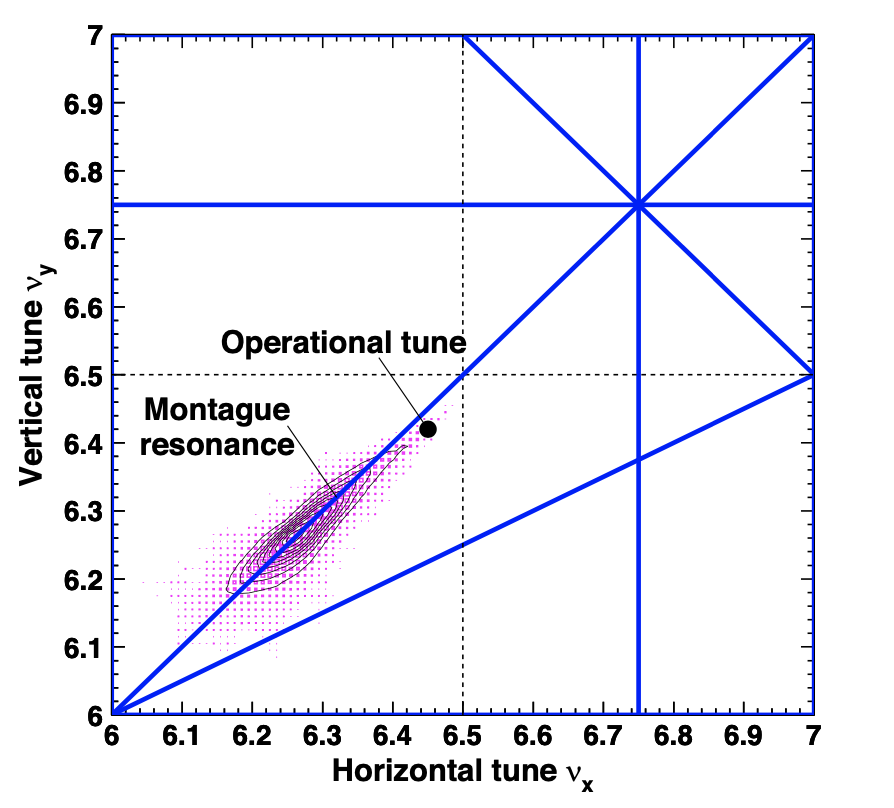
\includegraphics[width=0.6\textwidth]{Images/chapter1/montague.png}
    \caption{Simulated tune footprint in the JPARC accelerator. (From \cite{Hotchi2020})}
    \label{fig:jparc_montague}
\end{figure}
%

Thus, the beam intensity in rings is fundamentally limited by the incoherent space charge tune shift. A rough guideline is that the maximum tune shift should be kept below 0.25 to avoid fourth-order resonance lines \cite{book:Reiser}, but specific requirements depend on the application.


\subsubsection{Incoherent space charge resonances}

%
It is also possible for space charge itself to drive particle resonances \cite{Holmes1999, Jeon1999, Li2014, Kojima2019, Asvesta2020}. For illustration, we reproduce a numerical study from \cite{Hofmann2017Book} using PyORBIT \cite{Shishlo2015}, a particle-in-cell (PIC) code. Fig.~\ref{fig:incoherent_instability} shows a simulation of a truncated Gaussian distribution in a FODO lattice as the zero-current tune is decreased from 100\degree to 90\degree over 500 cells. The initial distribution has equal emittances in both planes and is matched to the lattice with a depressed tune of 92\degree.
%
\begin{figure}[!p]
    \centering
    \begin{subfigure}{\textwidth}
        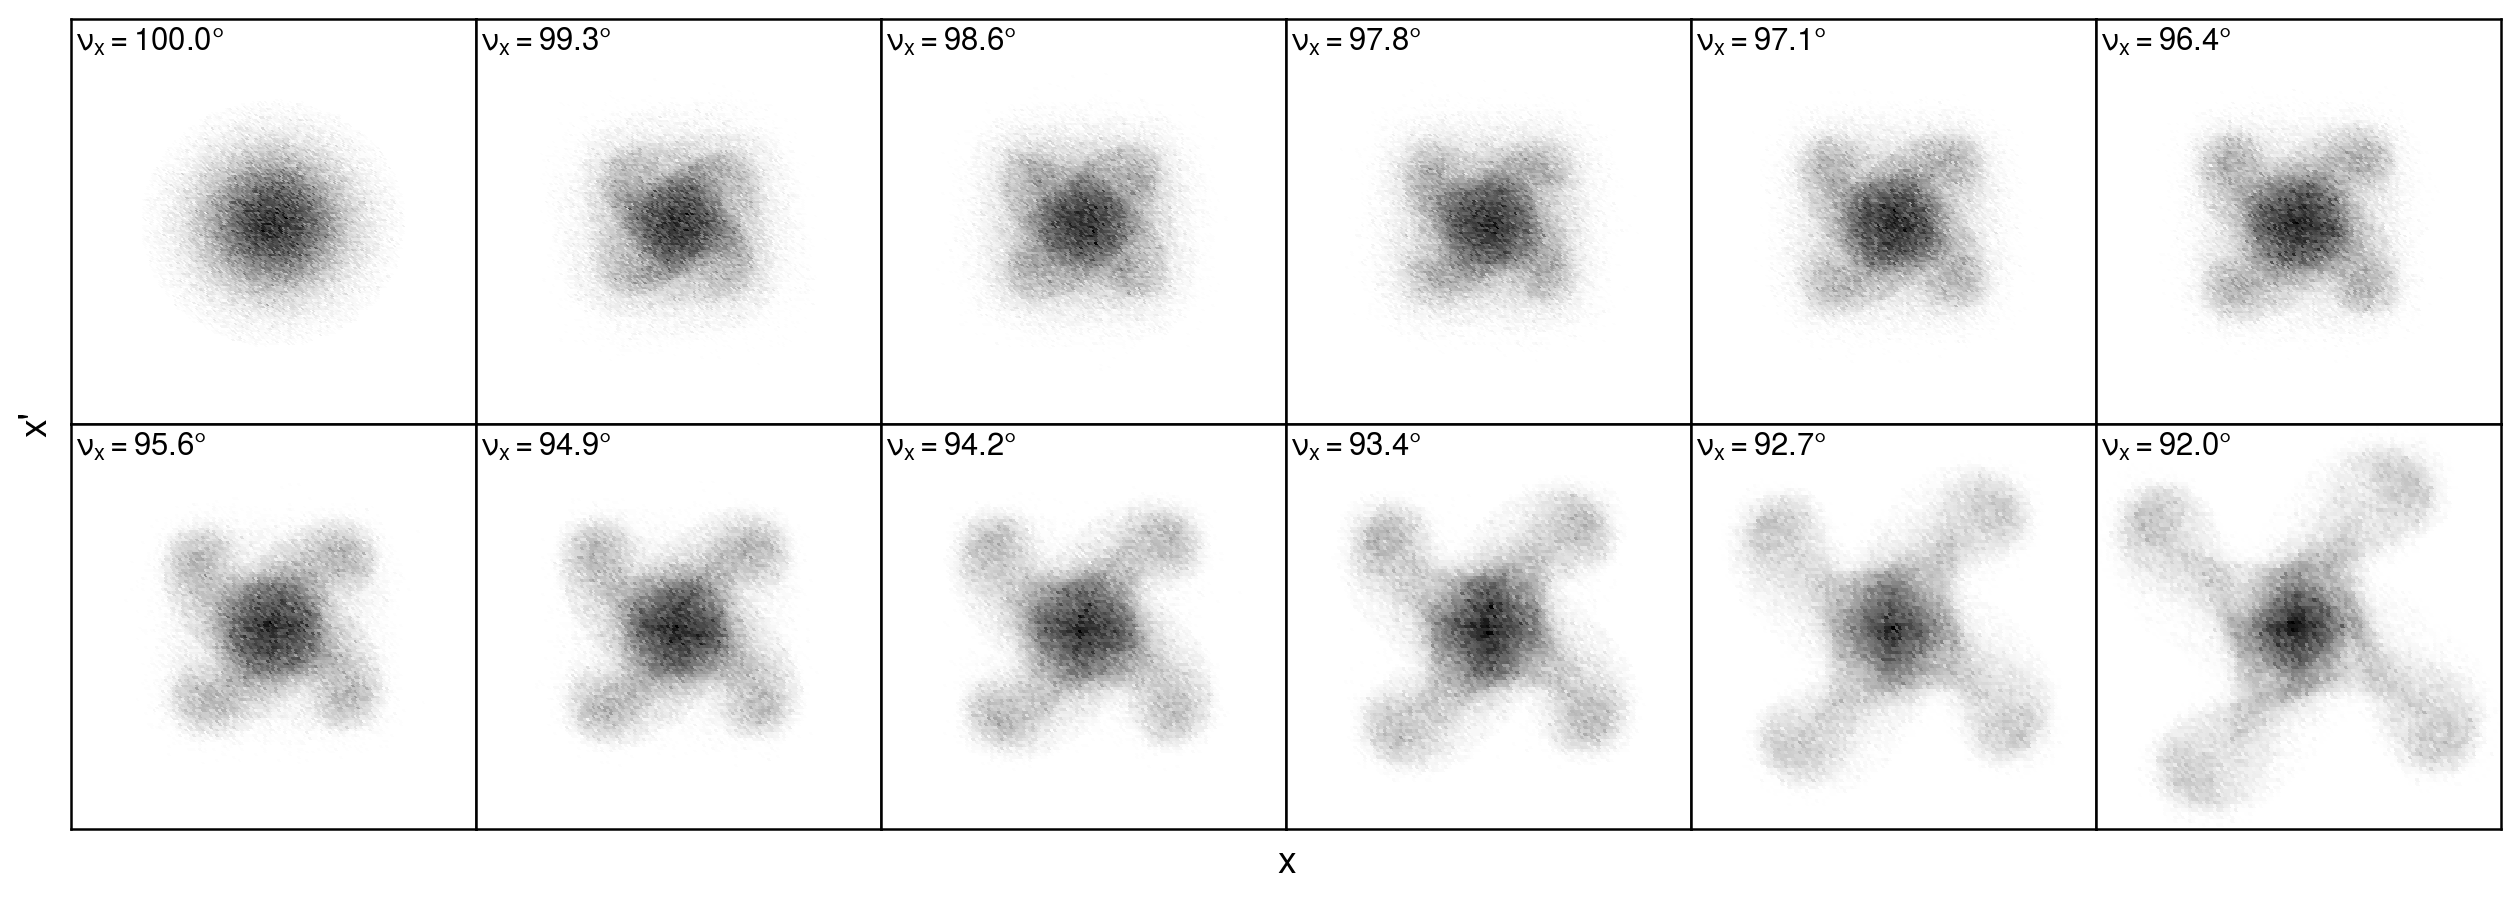
\includegraphics[width=\textwidth]{Images/chapter1/incoherent_resonance_fourth_order.png}
        \label{fig:incoherent_instability_a}
        \caption{}
    \end{subfigure}
    \begin{subfigure}{0.5\textwidth}
        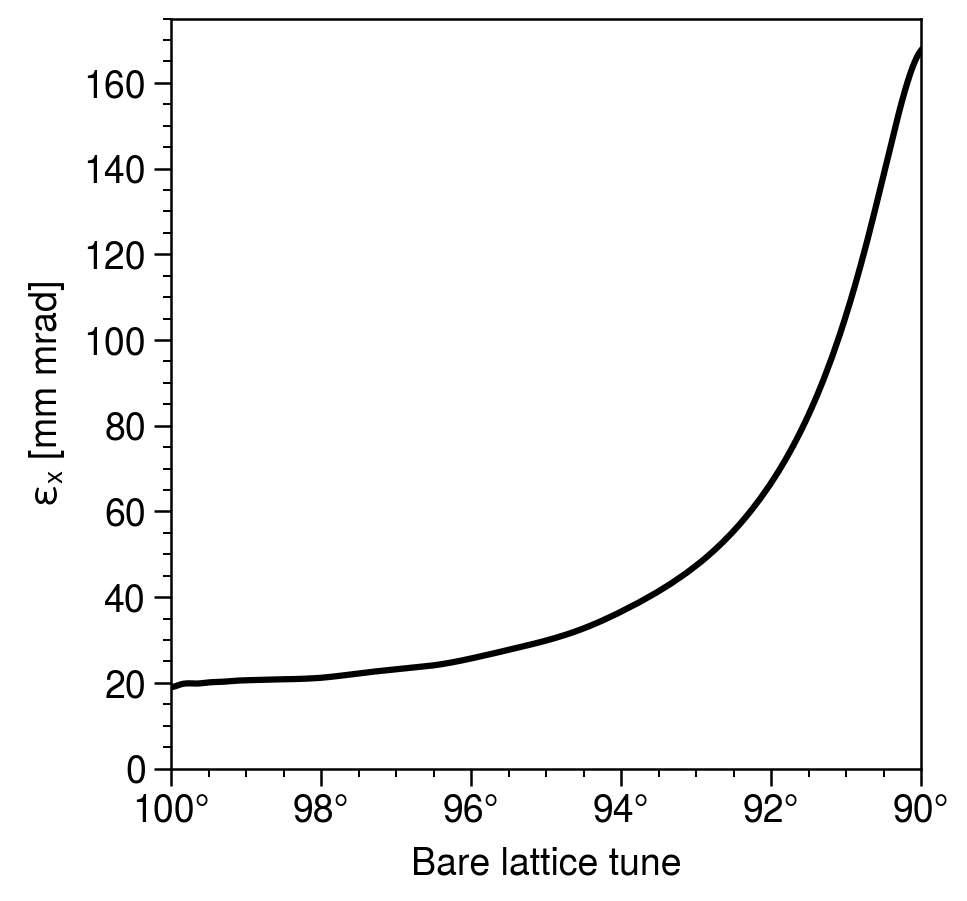
\includegraphics[width=\textwidth]{Images/chapter1/incoherent_resonance_fourth_order_emittance.png}
        \label{fig:incoherent_instability_b}
        \caption{}
    \end{subfigure}
    \caption{Simulation of a truncated Gaussian distribution in a FODO lattice. The zero-current tune is decreased from 100\degree to 90\degree over 500 cells. (a) $x$-$x'$ distribution. (b) RMS horizontal emittance. (Reproduced from \cite{Hofmann2017Book}.)}
    \label{fig:incoherent_instability}
\end{figure}
%
A fourth-order resonance is excited as the depressed tune approaches 90 degrees. The smooth emittance growth during most of the simulation shows that the core of the beam remains matched, justifying the use of ``incoherent" to describe the effect. Higher-order resonances can also occur for different combinations of beam intensity and focusing strength.


\subsection{Coherent effects}

Coherent space charge effects involve self-consistent oscillations of the entire beam and are relevant for strong space charge \cite{book:Reiser, Wangler2008, Cousineau2003}. We may model the beam as a smooth distribution in phase space $f(\mathbf{x})$; neglecting collisions between particles, the evolution of $f$ is given by the Vlasov equation \cite{Vlasov1961}:
%
\begin{equation} \label{eq:Vlasov}
    \frac{d}{ds}{f(\mathbf{x}, \mathbf{x}', s)} = 
    \frac{\partial{f}}{\partial{s}} +
    \mathbf{x}' \cdot \frac{\partial{f}}{\partial{\mathbf{x}}} +
    \mathbf{x}'' \cdot \frac{\partial{f}}{\partial{\mathbf{x'}}}
    = 0,
\end{equation}
%
where $\mathbf{x} = (x, y)^T$. Hidden in Eq.~\eqref{eq:Vlasov} is the single-particle equation of motion, which for linear external fields is:
%
\begin{equation}
    \mathbf{x}'' + \mathbf{K_0} \mathbf{x} + \mathbf{K_1} \mathbf{x}'
    =
    \frac{q}{m\gamma^3\beta^2c^2} \frac{\partial{\Phi}}{\partial\mathbf{x}},
\end{equation}
%
where $\mathbf{K}_{0, 1}$ are $2 \times 2$ matrices encompassing the external fields, and the space charge potential $\Phi$ is determined from the Poisson equation:
%
\begin{equation} \label{eq:Poisson}
    \frac{\partial^2{\Phi}}{\partial{\mathbf{x}^2}} = -\frac{q}{\epsilon_0}\int_{-\infty}^{\infty}{f}d\mathbf{x}'.
\end{equation}
%

Equilibrium solutions to the Vlasov equation in the presence of time-dependent linear forces are discussed in the following section. For now, we take it for granted that there exists one such solution, called the KV distribution, that produces linear space charge forces ($E_x \propto x$, $E_y \propto y$). In \cite{Hofmann1983}, Hofmann et al. analytically studied perturbations of a round ($\varepsilon_x = \varepsilon_y$) KV distribution using the Vlasov equation in one of the simplest time-dependent cases: a FODO lattice with equal horizontal and vertical tunes. The result is shown in Fig.~\ref{fig:stopbands}, which plots the depressed tune as a function of beam intensity. Each thin line represents a different zero-current tune. The thick lines represent regions of instability.
%
\begin{figure}[!p]
    \centering
    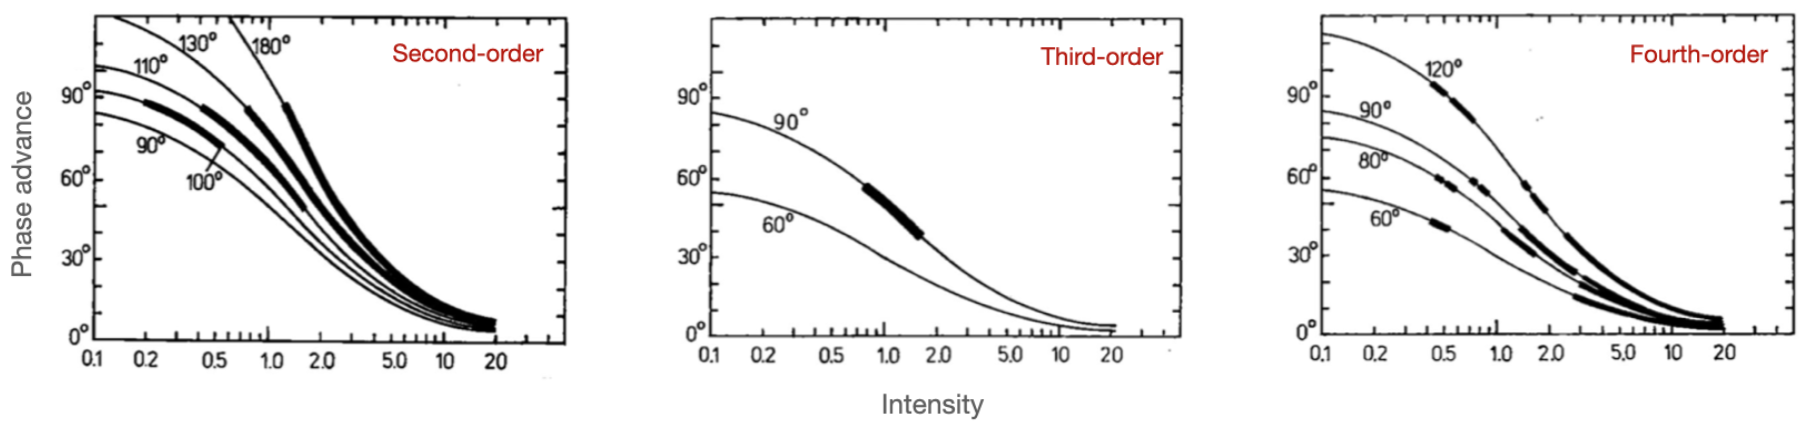
\includegraphics[width=\textwidth]{Images/chapter1/stopbands_hor.png}
    \caption{Instability stopbands obtained from perturbations of a KV distribution with equal emittances in a FODO lattice. (From \cite{Hofmann1983}).}
    \label{fig:stopbands}
\end{figure}
%
\begin{figure}[!p]
    \centering
    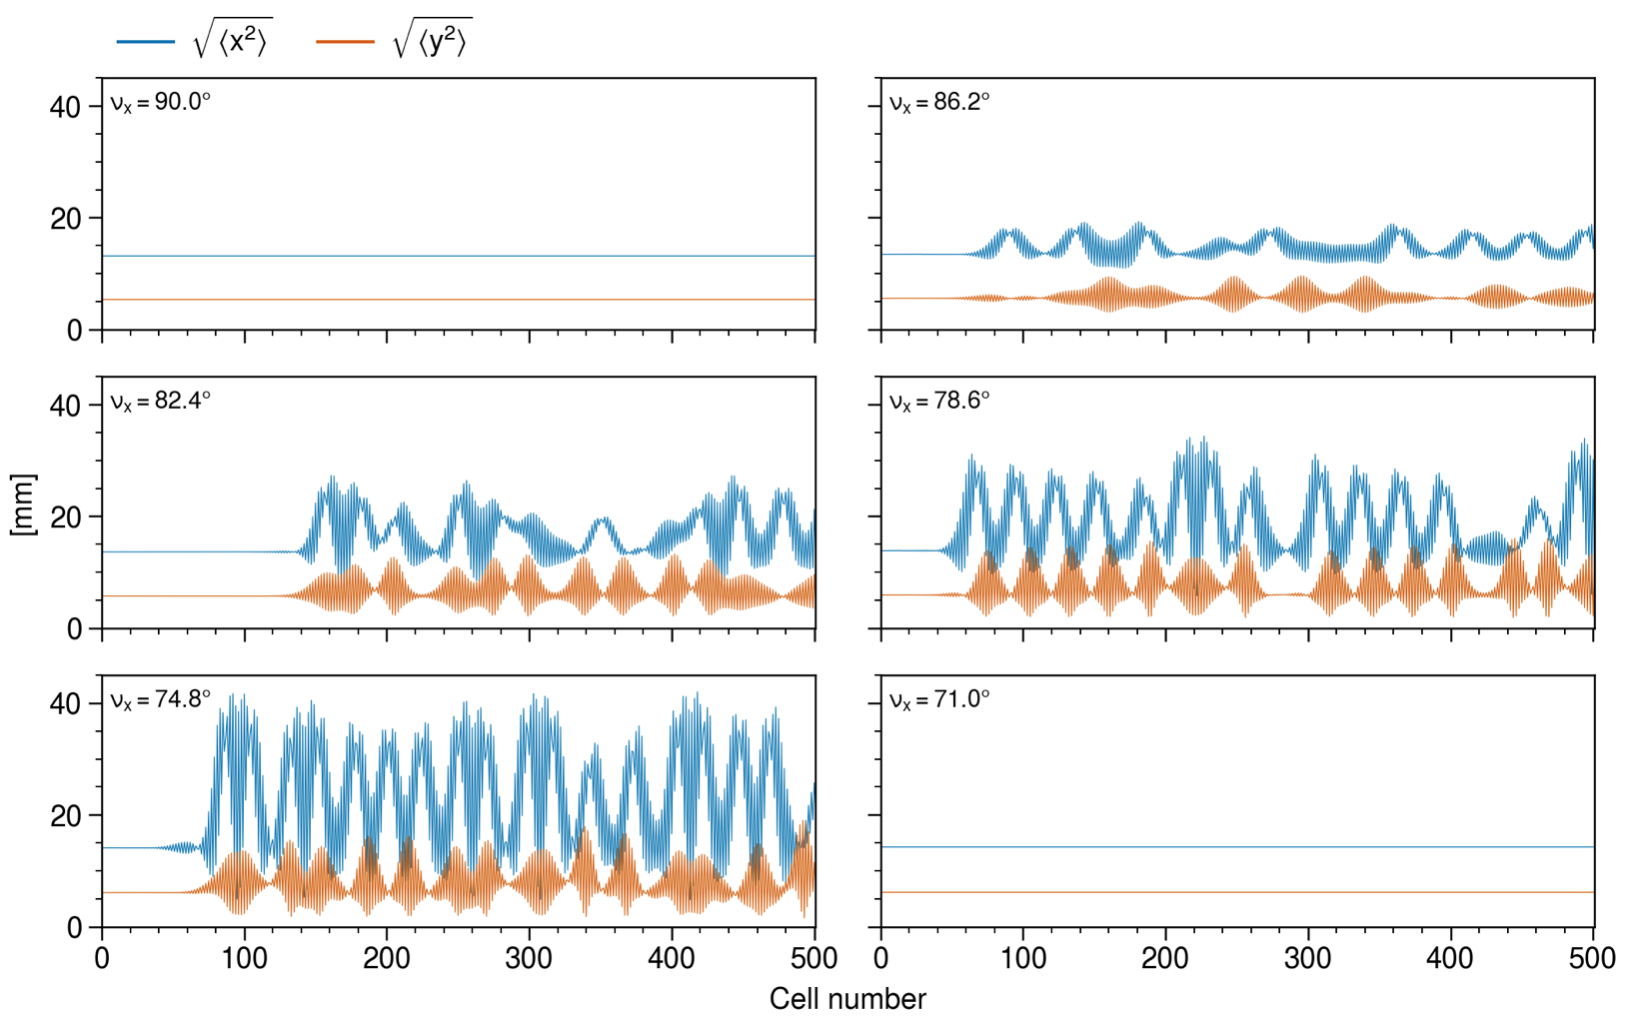
\includegraphics[width=\textwidth]{Images/chapter1/envelope_instability.png}
    \caption{Integrated KV envelope equations in a FODO lattice as the depressed KV tune $\nu_x$ is decreased. The zero-current tune is 100\degree.} \label{fig:envelope_instability}
\end{figure}
%

The KV distribution produces a closed set of differential equations for its envelope — the elliptical boundary containing the beam particles — due to its linear space charge forces. The second-order instabilities involve linear forces only, so they appear in the envelope equations. We use a FODO cell with a zero-current tune of $100\degree$ corresponding to the second-to-bottom line on the left-most plot in Fig.~\ref{fig:stopbands}. The initial distribution is first matched to the lattice, then tracked for 500 cells by integrating the KV envelope equations. Fig.~\ref{fig:envelope_instability} shows the horizontal and vertical envelopes as the depressed KV tune is decreased from $90\degree$ to $71\degree$, crossing the stopband. This is known as the envelope instability. It is assumed to be real, but its existence has not yet been experimentally confirmed.

Observation of the higher-order stopbands requires PIC simulation. We choose a zero-current tune of 90\degree; according to Fig.~\ref{fig:stopbands}, a third-order and fourth-order instability should occur at a depressed tune of 45\degree and 30\degree, respectively. Fig.~\ref{fig:coherent_instabilities} shows the simulated evolution in PyORBIT for three different distributions: KV, Waterbag, and Gaussian. (Note that while the simulations in \cite{Hofmann2017Book} used a bunched beam, coasting beams were used in this simulation.)
%
\begin{figure}[!p]
    \begin{subfigure}[b]{0.45\textwidth}
        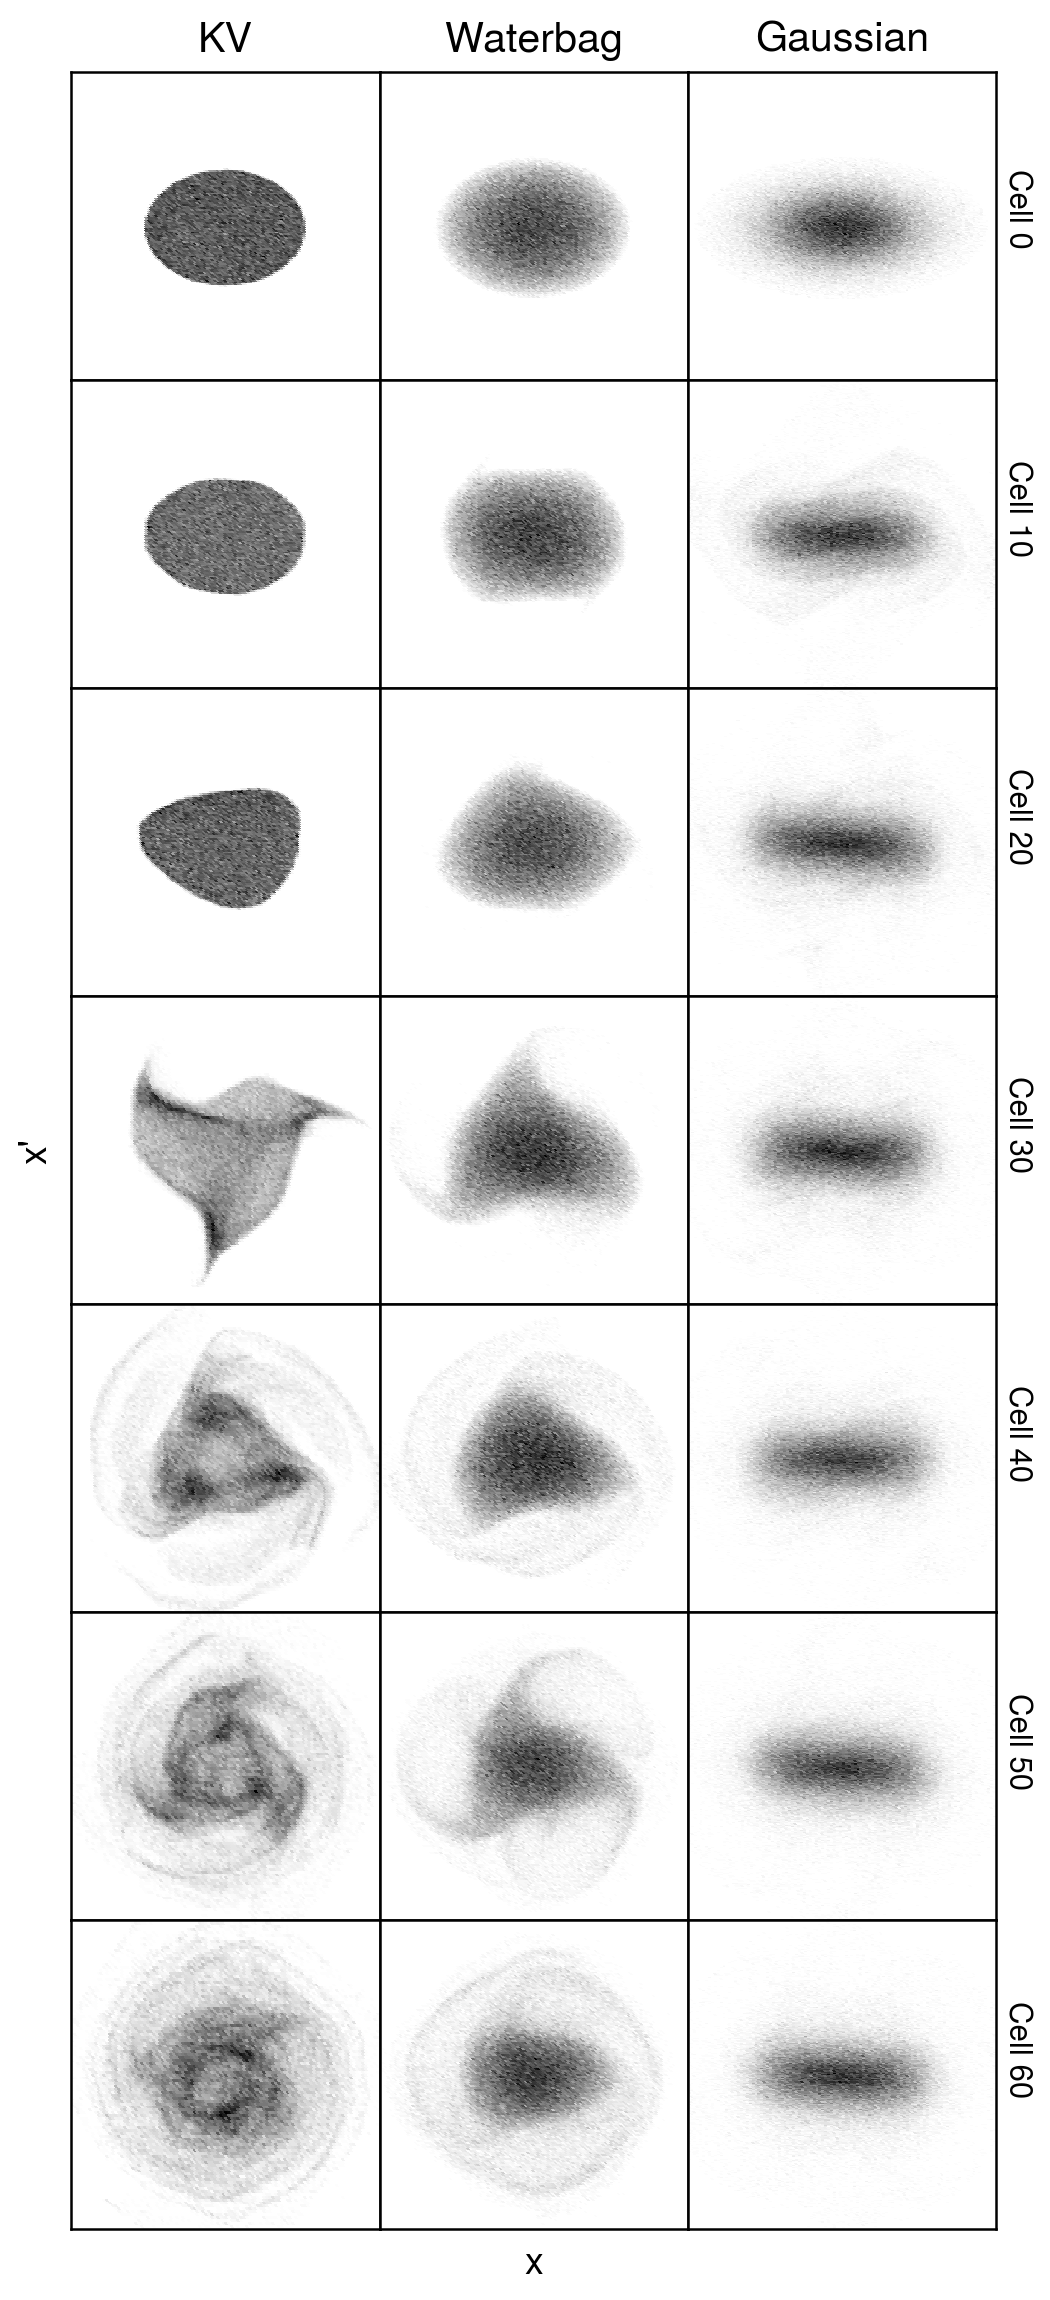
\includegraphics[width=\textwidth]{Images/chapter1/coherent_instability_fourth_order.png}
        \label{fig:coherent_instabilities_a}
    \end{subfigure}
    \hfill
    \begin{subfigure}[b]{0.45\textwidth}
        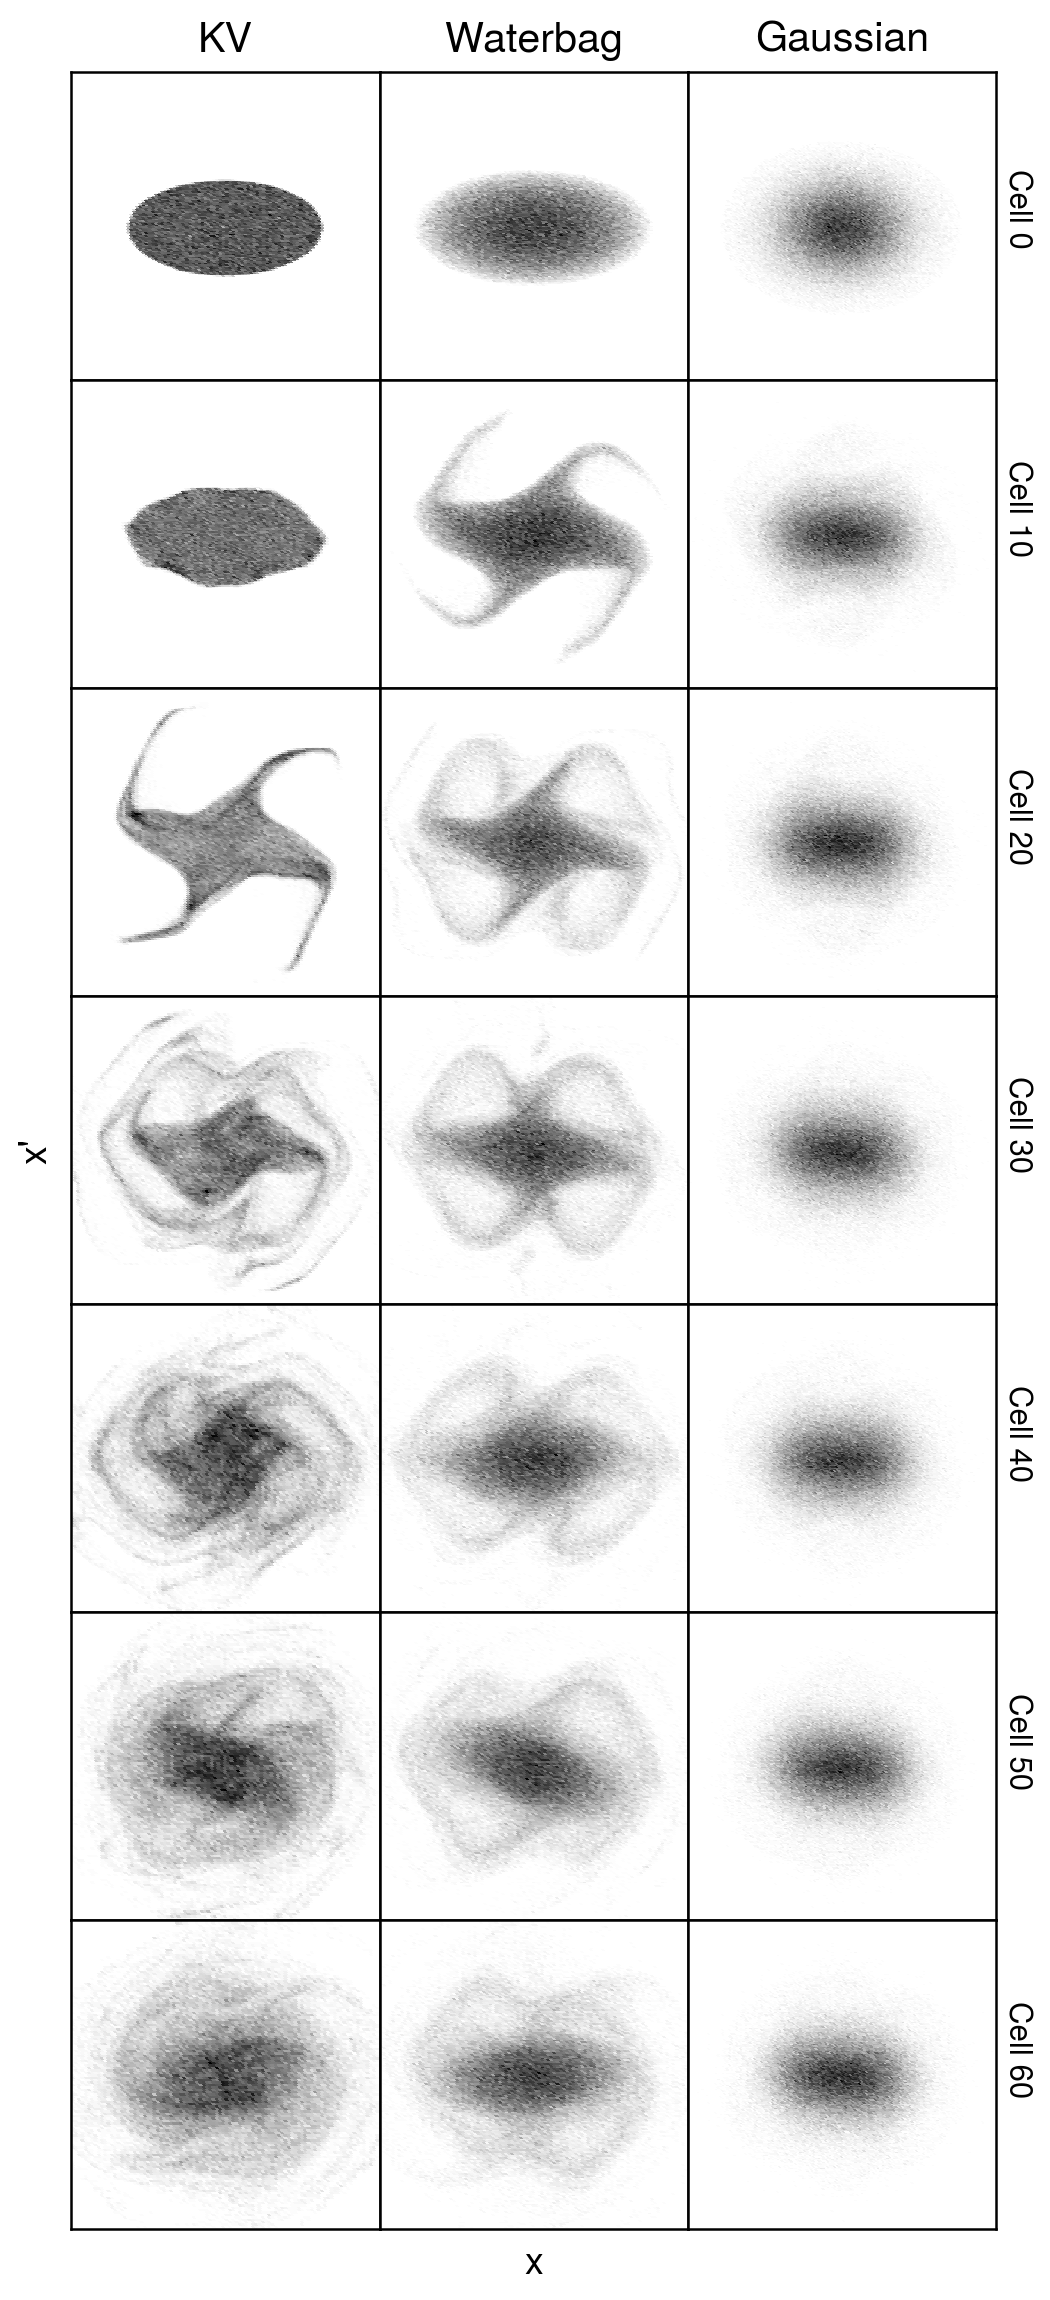
\includegraphics[width=\textwidth]{Images/chapter1/coherent_instability_third_order.png}
        \label{fig:f2}
    \end{subfigure}
    \vfill
    \begin{subfigure}[b]{\textwidth}
        \centering
        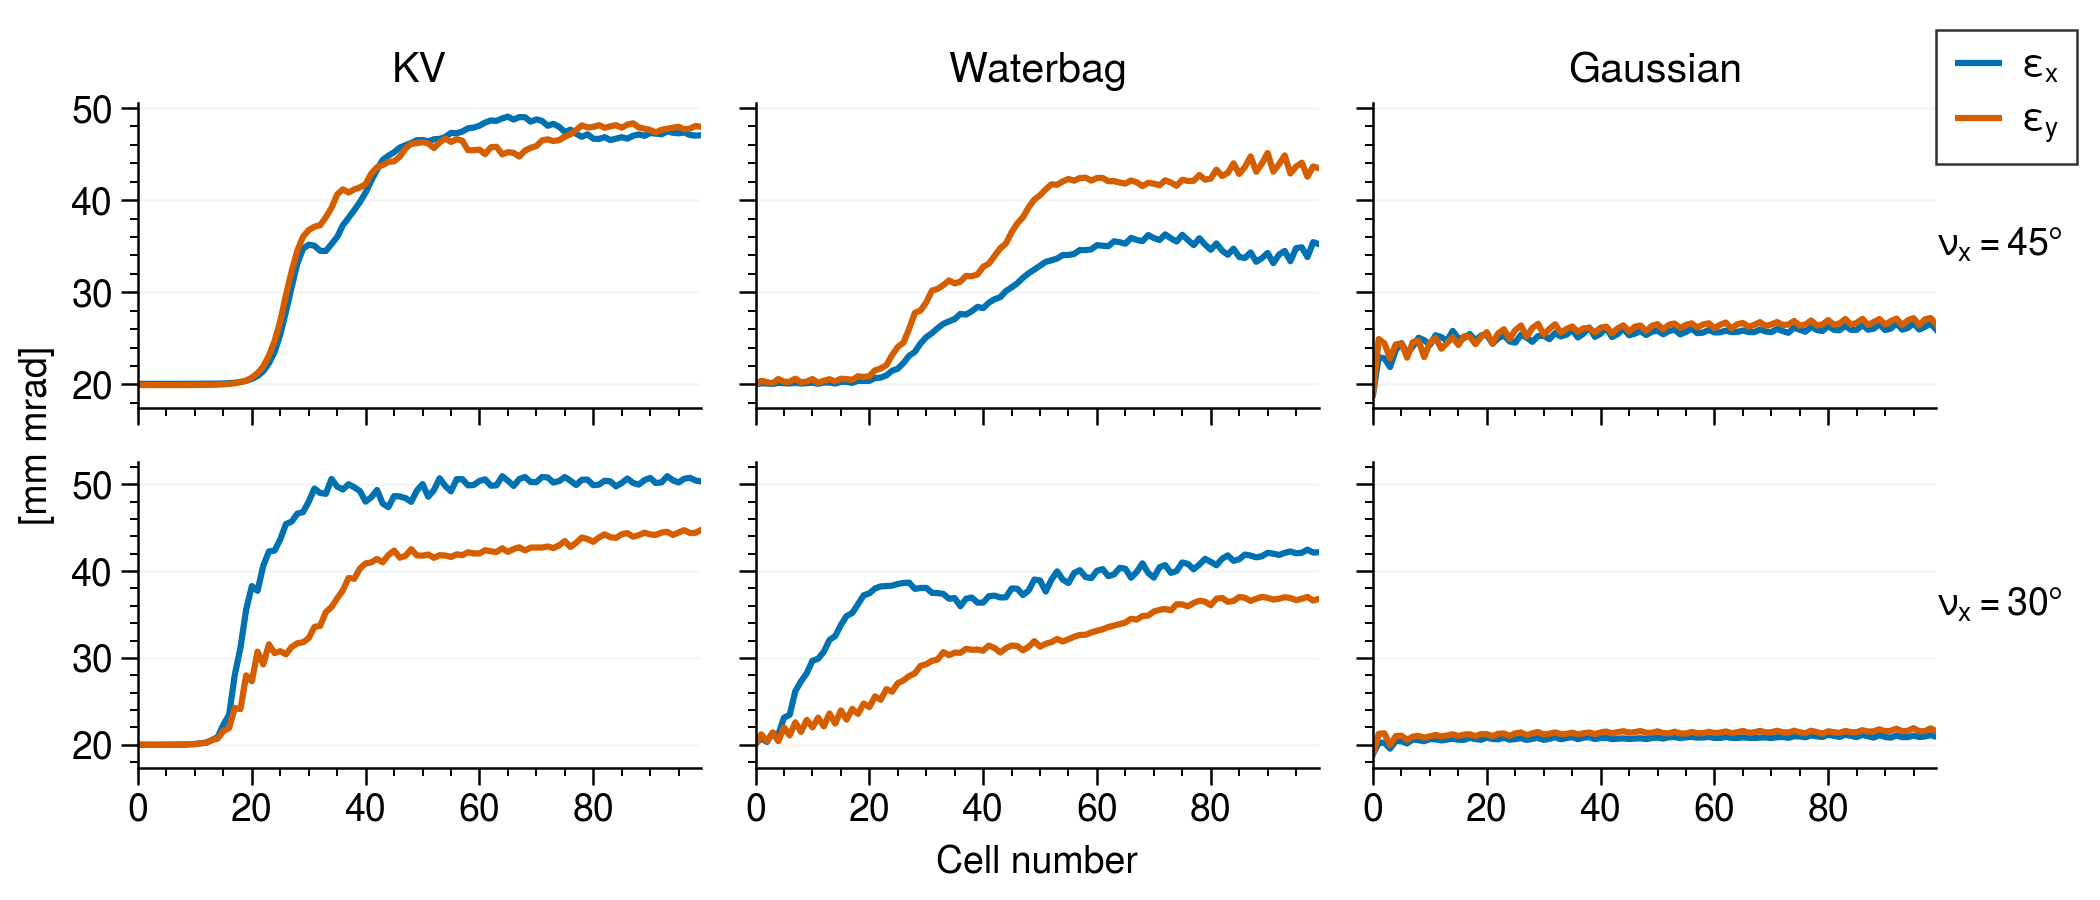
\includegraphics[width=0.8\textwidth]{Images/chapter1/coherent_instability_emittances.png}
        \label{fig:coherent_instabilities_b}
    \end{subfigure}
    \caption{Simulated Gaussian, Waterbag, and KV distributions in a FODO lattice with a zero-current tune of 90\degree and depressed KV tunes of $\nu_x$ = 45\degree (top left) and 30\degree (top right).}
    \label{fig:coherent_instabilities}
\end{figure}
%
The instabilities violently affect the KV distribution, but their effect is less pronounced in the other distributions. Thus, it is assumed that high-order coherent instabilities, while interesting, are not important in real beams with a large tune spread. 



\section{Self-consistent phase space distributions}\label{sec:Self-consistent phase space distributions}

\subsection{Definition and properties}

Any function constructed from single-particle invariants $\{C_i\}$ is an equilibrium solution to the Vlasov equation:
%
\begin{equation}\label{eq:vlasov_equilibria}
    \frac{d}{ds} f(\{C_i\}) = \sum_{i}{\frac{df}{dC_i}\frac{dC_i}{ds}} = 0.
\end{equation}
%
One example of a single-particle invariant when the focusing is linear and time-dependent is the Courant-Snyder invariant of Eq.~\eqref{eq:CS invariant}. The inclusion of space charge complicates the identification of invariants; the only known equilibrium distributions are those that produce linear space charge forces. We label such distributions as \textit{self-consistent}: a self-consistent distribution produces linear space charge forces, and the linearity of the space charge force is conserved under any linear transformation. 
Self-consistent distributions possess several notable properties. First, the integro-differential system of equations in Eq.~\eqref{eq:Vlasov} is reduced to a system of ordinary differential equations. Second, nonlinear space charge effects are minimized: the emittance is conserved, the maximum space charge tune shift is minimized, and the space charge tune spread is eliminated. Third, higher-order coherent instabilities may be present in self-consistent distributions due to their small tune spread. Fourth, self-consistent distributions give rise to a uniform charge density.



\subsection{Known solutions}

Danilov et al. enumerated a class of self-consistent distributions in $2d$-dimensional phase space \cite{Danilov2003}: 
%
\begin{equation}\label{eq:scdist_general_form}
    f\left({\mathbf{x}, \mathbf{x}'}\right) = 
    g\left({H - H_b}\right)
    \prod_{i=1}^{m}\delta\left({\mathbf{e}_i \cdot \mathbf{x} 
    + \mathbf{e}'_i \cdot \mathbf{x}'}\right),
\end{equation}
%
where $\mathbf{x}$, $\mathbf{x}'$ are the $d$ dimensional vector coordinates and momenta, $g$ is a function of $H$ — a quadratic positively defined function of the phase space coordinates — and $H_b$ — an upper bound on $H$ — $\delta$ is the Dirac delta function, and $\mathbf{e}_i$, $\mathbf{e}'_i$ are vectors of constants. This is referred to as the $\{n,m\}$ case. It was proven that the electric field within any uniformly filled ellipsoid is linear, and that any distribution of the form of $\eqref{eq:scdist_general_form}$ that produces a linear electric field will do so under any linear transformation.


In other words, one class of self-consistent distributions are those that generate linear space charge forces and are constructed from quantities that are invariant in the presence of linear focusing. We now focus on the \{2, 0\} and \{2, 2\} cases. (Qin and Davidson derived a self-consistent distribution for $n = 2$ in \cite{Qin2013} using their recent parameterization of coupled motion, but made no reference to \cite{Danilov2003}. The connection between Danilov's work and Qin and Davidson's work should thus be explored in the future.)


\subsubsection{The KV distribution}

The $\{2, 0\}$ case corresponds to the KV distribution derived by Kapchinskij and Vladimirskij in 1959 \cite{Kapchinskij1959}. The distribution is a function of the Courant-Snyder invariants $J_x$ and $J_y$:
%
\begin{equation}
    f(\mathbf{x}, \mathbf{x}') = \frac{\lambda}{\pi^2 \varepsilon_x\varepsilon_y}
    \delta \left(\frac{J_x}{\varepsilon_x} + \frac{J_y}{\varepsilon_y} -1 \right),
\end{equation}
%
where $\lambda$ is the longitudinal particle density. Particles in the KV distribution are evenly distributed on an ellipsoidal shell in 4D phase space. As shown in Fig.~\ref{fig:distributions_kv}, any 2D projection of the distribution is a uniform density ellipse. Of particular importance is the $x$-$y$ projection, which remains upright and uniform density under any uncoupled transformation. The electric field within such an ellipse is
%
\begin{equation}  \label{eq:field_in_upright_ellipse}
    \mathbf{E}(x, y) =
    \frac{\lambda}{\pi\epsilon_0}
    \left[ 
        \frac{x}{c_x\left(c_x+c_y\right)} \hat{x}
        + \frac{y}{c_y\left(c_x+c_y\right)} \hat{y}
    \right],
\end{equation}
%
where $c_x$ and $c_y$ are the horizontal and vertical semi-axes and $\epsilon_0$ is the permittivity of free space. Since the space charge force is linear and uncoupled, $J_{x,y}$ remains invariant for every particle and the emittances $\varepsilon_{x,y}$ are conserved. The KV distribution does not exist in 3D \cite{Sacherer1968}.

As mentioned in the previous section, the preservation of the linearity of the space charge force leads to a self-consistent set of differential equations for the evolution of the beam envelope. The KV envelope equations read:
%
\begin{align} \label{eq:KV_envelope}
    \tilde{x}'' + k_{x}(s)\tilde{x} - \frac{\varepsilon_x^2}{\tilde{x}^3} - \frac{Q}{2\left(\tilde{x} + \tilde{y}\right)} &= 0, \\
    \tilde{y}'' + k_{y}(s)\tilde{y} - \frac{\varepsilon_y^2}{\tilde{y}^3} - \frac{Q}{2\left(\tilde{x} + \tilde{y}\right)} &= 0. \nonumber
\end{align}
%
The RMS widths of the beam $\tilde{x} = \sqrt{\langle{{x^2}}}$ and $\tilde{y} = \sqrt{\langle{{y^2}}}$ are used instead of the true widths $c_x$ and $c_y$. They are simply related by a factor of two for a uniform density ellipse. The perveance $Q$ is a dimensionless measure of space charge strength:
%
\begin{equation}\label{eq:perveance}
    Q = \frac{2\lambda r_0}{\beta^2\gamma^3},
\end{equation}
%
where $r_0 = e^2 / 4\pi\epsilon_0mc^2$ is the classical proton radius. Eqs.~\eqref{eq:KV_envelope} provide many insights into dynamical beam behavior and an analytic benchmark for computer simulations.  

A remarkable fact is that Eqs.~\eqref{eq:KV_envelope} are exact for distributions with elliptical symmetry even if the space charge force is nonlinear \cite{Sacherer1968}. They are not closed, however, since the emittances would then depend on time. Thus, the KV envelope equations provide a good approximation to the evolution of more realistic distributions in the limit of elliptical symmetry and small emittance growth \cite{Lund2004}.


\subsubsection{The Danilov distribution}

The focus of this dissertation is on the $\{2, 2\}$ case of Eq.~\eqref{eq:scdist_general_form} which will be referred to as the Danilov distribution:
%
\begin{equation}
    f(\mathbf{x}, \mathbf{x}') \propto 
    \Theta\left({1 - \mathbf{x}^T\bm{\mathbf{\sigma}^{-1}}\mathbf{x}}\right)
    \delta\left({\mathbf{x} - \mathbf{D}\mathbf{x}'}\right)
\end{equation}
%
with 
%
\begin{equation}
    \bm{\sigma} = 
    4
    \begin{bmatrix}
        \langle{xx}\rangle & \langle{xy}\rangle \\
        \langle{xy}\rangle & \langle{yy}\rangle
    \end{bmatrix}
\end{equation}
%
and $\mathbf{D}$ a $2 \times 2$ matrix. Similar to the KV distribution, any 2D projection of the Danilov distribution is a uniform density ellipse; however, the ellipses in the cross-plane projections ($x$-$y$, $x$-$y'$, $y$-$x'$, $x'$-$y'$) are not necessarily upright and may collapse to lines. For example, the projections are shown in Fig.~\ref{fig:distributions_danilov} for $\mathbf{D}_{11}=\mathbf{D}_{22}=0$ and $\mathbf{D}_{12} = -\mathbf{D}_{21}=1$, which corresponds to a rigidly rotating disk. The electric field in a uniform density ellipse with semi-axes $c_{x,y}$ tilted at an angle $\phi$ in the $x$-$y$ plane is:
%
\begin{equation}
\begin{aligned}
    E_x &\propto 
    \left({\frac{\cos^2\phi}{c_x} + \frac{\sin^2\phi}{c_y}}\right) \frac{x}{c_x + c_y}
    +
    \sin\phi\cos\phi \left({\frac{1}{c_y} - \frac{1}{c_x}}\right) \frac{y}{c_x + c_y}, \\
    E_y &\propto 
    \left({\frac{\cos^2\phi}{c_y} + \frac{\sin^2\phi}{c_x}}\right) \frac{y}{c_x + c_y}
    +
    \sin\phi\cos\phi \left({\frac{1}{c_y} - \frac{1}{c_x} }\right) \frac{x}{c_x + c_y}.
\end{aligned}
\end{equation}
%
The field is linear in $x$ and $y$, as required. And it is worth repeating: the linearity of the electric field is maintained under any linear transformation. The key difference from the KV distribution is that space charge linearly couples the horizontal and vertical motion of individual particles. The Courant-Snyder invariants $J_{x,y}$ are therefore replaced by the more general invariants $J_{1, 2}$, which are conserved even with the inclusion of space charge. 

Due to the cross-plane correlation in the Danilov distribution, the 4D emittance is not the simple product of the horizontal and vertical emittances $\varepsilon_x$ and $\varepsilon_y$, which we refer to as the \textit{apparent} emittances from now on. Instead, the 4D emittance is the product of the \textit{intrinsic} emittances $\varepsilon_1$ and $\varepsilon_2$:
%
\begin{equation} \label{eq:mode_emittances1}
    \varepsilon_{4D} = \left|{\bm{\Sigma}}\right|^{1/2} = \varepsilon_1\varepsilon_2.
\end{equation}
%
The intrinsic emittances are found by a symplectic diagonalization of $\bm{\Sigma}$, i.e., they are the imaginary components of the eigenvalues of $\bm{\Sigma}\mathbf{U}$, where $\mathbf{U}$ is the unit symplectic matrix:
%
\begin{equation}
    \mathbf{U} = 
    \begin{bmatrix}
        0 & 1 & 0 & 0 \\
        -1 & 0 & 0 & 0 \\
        0 & 0 & 0 & 1 \\
        0 & 0 & -1 & 0
    \end{bmatrix}.
\end{equation}
%
The answer can be written compactly \cite{Xiao2013}:
%
\begin{equation}
    \varepsilon_{1, 2} = \frac{1}{2}\sqrt{
      -tr\left[(\bm{\Sigma} \mathbf{U})^2\right] \pm \sqrt{tr^2\left[(\bm{\Sigma} \mathbf{U})^2\right] - 16|{\bm{\Sigma}}|},
    }
\end{equation}
%
The intrinsic emittances are constants of the motion for any linear focusing system. Their product is less than or equal to the product of the apparent emittances \cite{Buon1993}. The delta functions in the Danilov distribution function cause the 4D emittance, and therefore one of the intrinsic emittances, to be zero. The following relationship holds:
%
\begin{equation} \label{eq:mode_emittances2}
    \varepsilon_1 = \varepsilon_x + \varepsilon_y, \quad
    \varepsilon_2 = 0
\end{equation}
%
or vice versa. 

Discussion of the Danilov envelope equations is reserved for chapter \ref{chap-2}.




\section{Producing a self-consistent distribution}\label{sec:Producing a self-consistent distribution}


\subsection{Motivation}

The following points motivate the physical realization of a self-consistent distribution.

\begin{enumerate}
\item 
The properties listed in section~\ref{sec:Self-consistent phase space distributions} — conservation of emittance, reduced space charge tune shift, and reduced space charge tune spread — have the potential to increase the maximum intensity in a ring.

\item
It is an interesting challenge to bring a real distribution closer to a self-consistent analytical model which is generally taken to be unrealistic. 

\item
Beams with a uniform charge density are ideal for fixed-target applications such as spallation neutron production. SNS targets are complex entities that cost \$$1.5 \times 10^6$ to replace, and considerable research and development goes into reducing the peak density on the target. This issue will become even more important if future machines are built on the intensity horizon with similar targets.

\item
There has been recent interest in generating circular modes, where a circular mode is a beam with small 4D emittance. Such a beam can be transformed to a round state ($\varepsilon_x = \varepsilon_y$) or a flat state ($\varepsilon_x \ll \varepsilon_y$) using coupled linear optics that preserve $\varepsilon_{1,2}$. In \cite{Burov2002}, several potential applications of circular modes are listed. Consider first a round-flat transformation. The fractional increase in beam luminosity — a figure of merit in colliders [\ref{}] — in this case is
%
\begin{equation}
    C = \sqrt{\frac{\varepsilon_x\varepsilon_y}{\varepsilon_1\varepsilon_2}},
\end{equation}
%
which approaches $\infty$ as $\varepsilon_1\varepsilon_2 \rightarrow 0$. Flat beams may also increase the possible beam intensity in a ring by suppressing incoherent space charge resonances in one dimension, freeing large areas of tune space. The possible uses of flat beams in the Large Hadron Collider (LHC) are suggested by Burov in \cite{Burov2013}. Alternatively, round beams may be helpful for the suppression of beam-beam effects at collider interaction points \cite{Danilo1996}. Circular modes may also find use in relativistic electron cooling \cite{Burov2000}, low-energy hadron cooling \cite{Derbenev2000}, muon ionization cooling, and radiation generation \cite{Corlett2001}. The connection between the Danilov distribution and circular modes is straightforward: the Danilov distribution is a circular mode with uniform charge density. 

\end{enumerate}

\subsection{Previous experimental work}

Luiten et al. proposed a method to create a \{3, 3\} distribution (a 3D uniform density ellipsoid) of electrons \cite{Luiten2004}. They observed that since a uniform density oblate spheroid ($(x/A)^2 + (y/B)^2 + (z/C)^2 = 1$ with $A = B > C$) will collapse under its own gravity into a flat disk \cite{Lin1965}, a flat transverse disk of electrons will longitudinally expand into a uniform density ellipsoid. This ``pancake" distribution can be created using ultrashort pulsed-laser photoemission with an appropriate radial intensity profile. Musumeci et al. experimentally demonstrated this method in \cite{Musumeci2008}. Their measurements are shown in Fig.~\ref{fig:Musumeci}.
%
\begin{figure}[!p]
    \centering
    \begin{subfigure}{0.75\textwidth}
        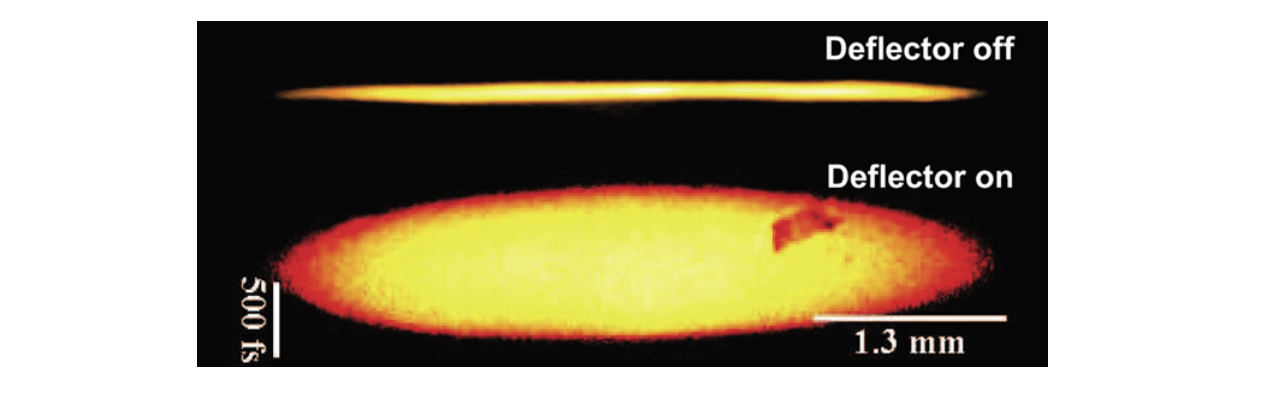
\includegraphics[width=\textwidth]{Images/chapter1/Musumeci_fig2.png}
        \label{fig:Musumeci_a}
        \caption{}
    \end{subfigure}
    \vfill
    \vspace*{1.5cm}
    \vfill
    \begin{subfigure}{0.75\textwidth}
        \centering
        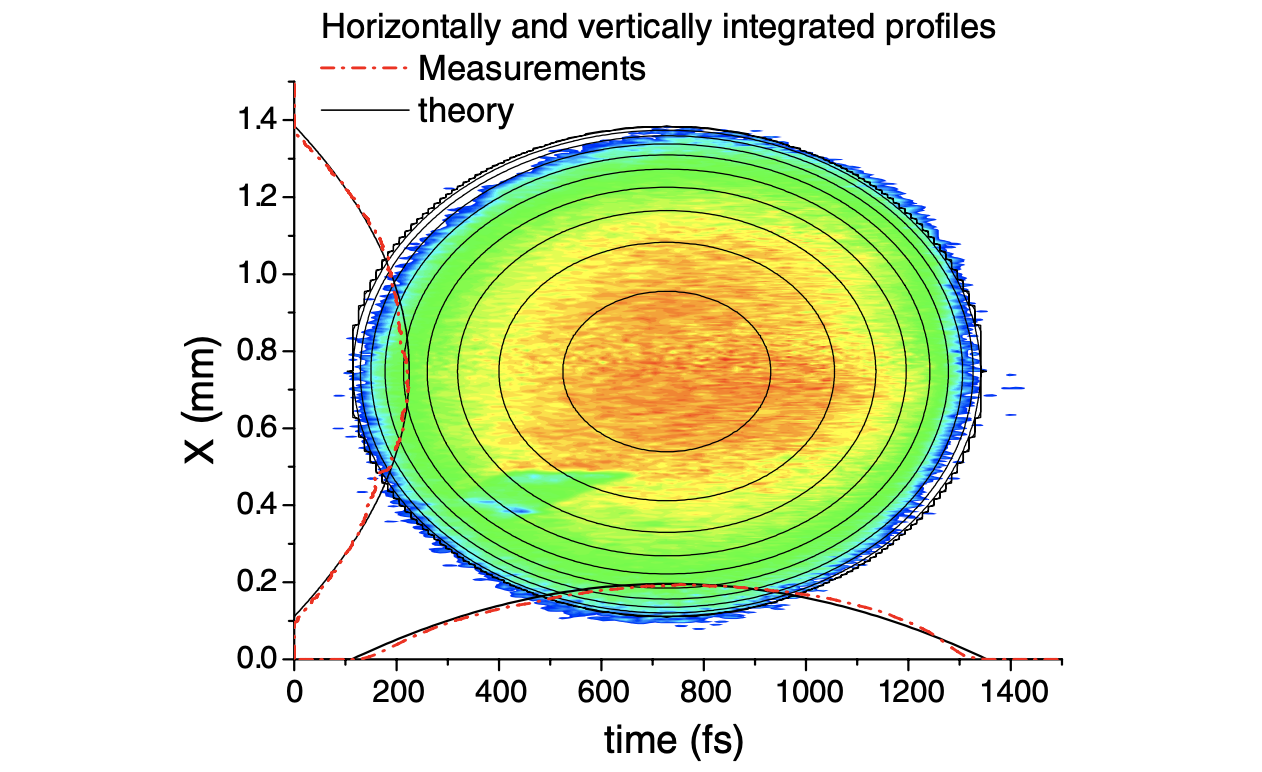
\includegraphics[width=\textwidth]{Images/chapter1/Musumeci_fig3.png}
        \label{fig:Musumeci_b}
        \caption{Lower image in (a), displayed with a different color map, and 1D projections of the image.}
    \end{subfigure}
    \caption{Measured electron beam images in the  $x$-$z$ plane from \cite{Musumeci2008}.}
    \label{fig:Musumeci}
\end{figure}
%

Unfortunately, these methods do not apply to high-intensity proton rings. Distributions in these machines are built up over many turns and can often be approximated as 2D coasting beams. The rest of this section describes a method to generate a Danilov distribution in a high-intensity proton ring using the concept of phase space painting, as well as the implementation of the method in the SNS.


\subsection{Phase space painting}

Accelerators are often broken into stages; a common pattern is the injection of a beam from a linac into a ring followed by eventual extraction to a different section of the machine. Injection and extraction are accomplished using kicker magnets — dipole magnets with fast rise times.

In multi-turn injection, multiple beam pulses are injected into the same stable region of longitudinal phase space in the ring. This process is limited by Liouville's theorem in the sense that the phase space density in the ring cannot be increased. In charge-exchange injection, an ion beam from the linac is stripped of its electrons upon entering the ring, leaving only protons. This produces a higher phase space density because charge-exchange is a non-Liouvillian process. While multi-turn injection is constrained to tens of turns, charge-exchange injection is performed over hundreds of turns \cite{Bracco2017}.

Phase space painting — or simply ``painting" — is the time-dependent variation of the transverse distance and angle between the injected beam and the circulating beam; as such, it allows time-dependent control over the phase space distribution in the ring. Painting is a vital tool for the mitigation of space charge effects in high-intensity rings. The free parameters are the painting path — the path of the injection point in phase space — and the speed at which this path is traversed. After discussing the two most popular painting methods, we will introduce a new method called elliptical painting that theoretically produces a Danilov distribution.


\subsection{Square root painting methods}

Although particles move along elliptical trajectories in $x$-$x'$ and $y$-$y'$ phase space in the linear approximation, they explore a rectangular region in the $x$-$y$ plane due to differences in the horizontal and vertical tunes. Square root painting methods make the best of this situation by theoretically generating uniform density ellipses in $x$-$x'$ and $y$-$y'$ phase space. 

\subsubsection{Correlated painting}

Let $x$, $x'$, $y$, and $y'$ be the coordinates of the injected beam in the phase space of the circulating beam, and $t$ be a time variable normalized to the range [0, 1]. In its simplest form, correlated painting proceeds as
%
\begin{equation}
\begin{aligned}
    {x}(t) &= {x}_{max}\sqrt{t}, \\
    {y}(t) &= {y}_{max}\sqrt{t}.
\end{aligned}
\end{equation}
%
In the linear approximation and without space charge, correlated painting generates uniform density ellipses in the $x$-$x'$ and $y$-$y'$ planes and a rectangular distribution in the $x$-$y$ plane. This is illustrated on the left side of Fig.~\ref{fig:painting_graphic}.
%
\begin{figure}[!p]
    \centering
    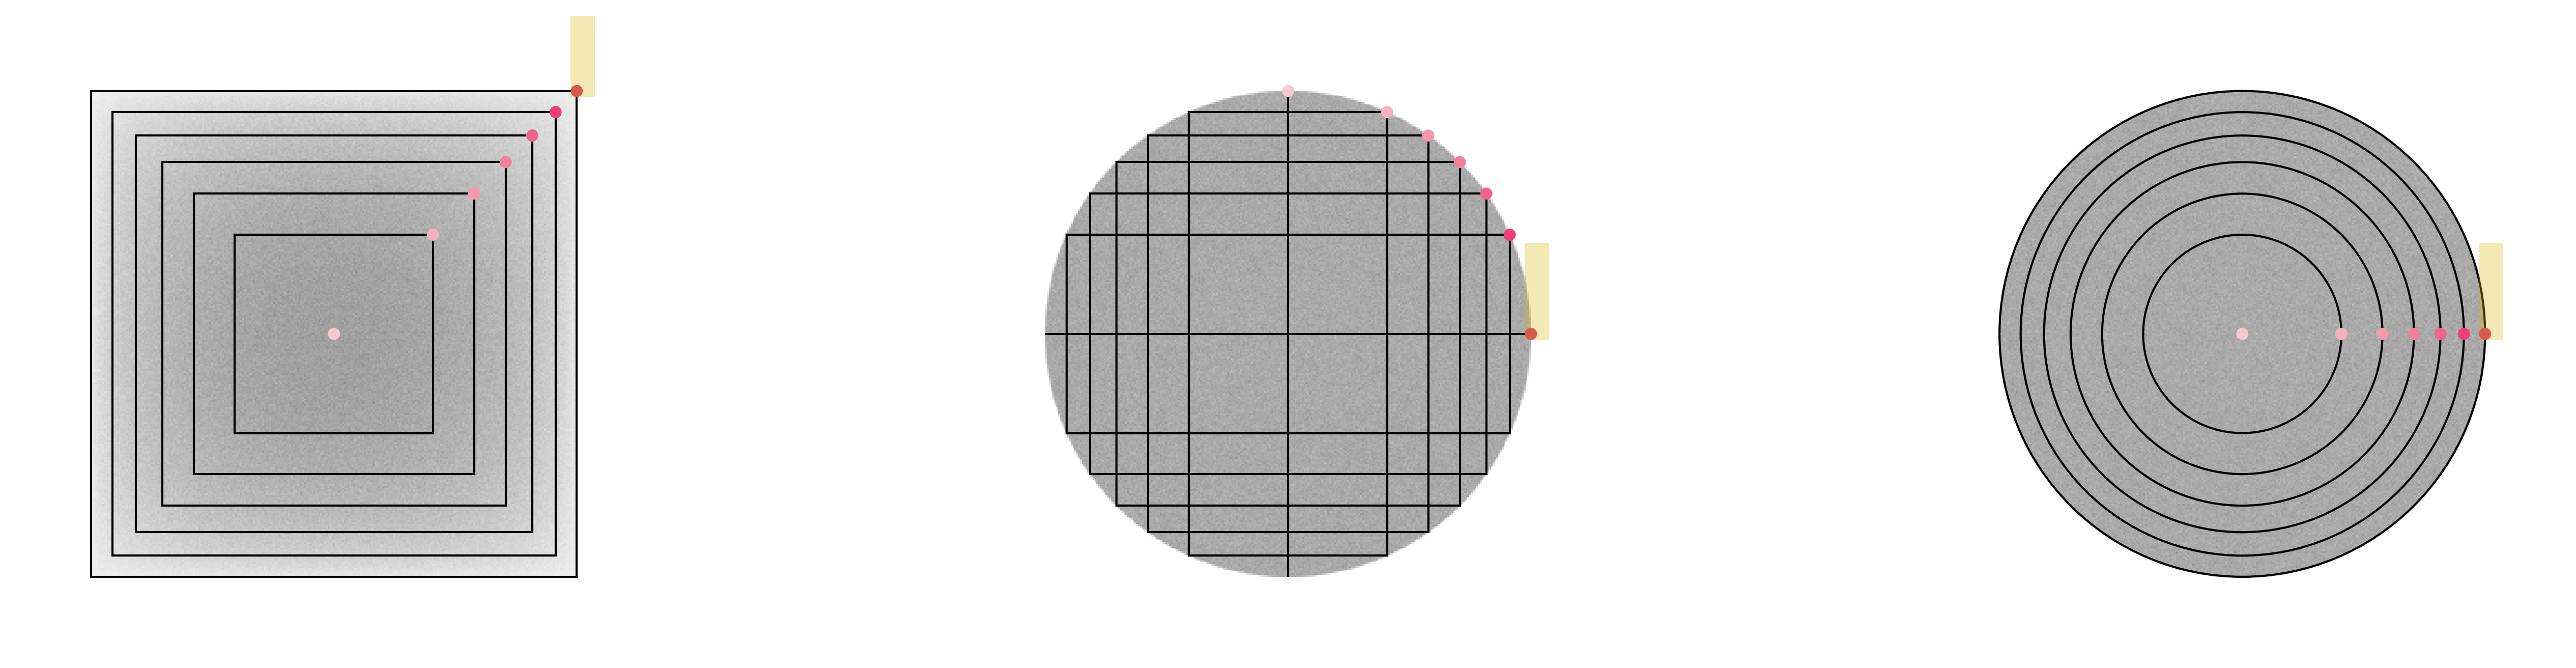
\includegraphics[width=\textwidth]{Images/chapter1/painting_graphic.png}
    \caption{Illustration of correlated painting (left), anti-correlated painting (center), and elliptical painting (right) in the linear approximation without space charge.}
    \label{fig:painting_graphic}
\end{figure}
%
But note that the 1D projection of a uniform density ellipse is a parabola, but the 1D projection of a uniform density rectangle is flat-topped. So the density in the $x$-$y$ plane is non-uniform, leading to nonlinear space charge forces.

A primary concern in the SNS is the size and peak density of the $x$-$y$ distribution on the spallation target \cite{Riemer2010}. A modified correlated painting scheme is employed to this end:
%
\begin{equation}
\begin{aligned}
    {x}(t) &= x_0 + x_{max}\sqrt{t}, \\
    {y}(t) &= y_0 + y_{max}\sqrt{t}. \\
\end{aligned}
\end{equation}
%
Initially, a donut is created in phase space. Space charge and other nonlinear forces eventually cause the distribution to fill in its hollow center, reducing the peak density.


\subsubsection{Anti-correlated painting}

Anti-correlated painting is equivalent to correlated painting reversed in one of the planes:
%
\begin{equation}
\begin{aligned}
    {x}(t) &= x_{max}\sqrt{t}, \\
    {y}(t) &= y_{max}\sqrt{1 - t}. \\
\end{aligned}
\end{equation}
%
Initially, the $x$-$x'$ distribution is a point while the $y$-$y'$ distribution is a donut. The painting path in this method follows the line $J_x + J_y = constant$, which is the condition of particles in the KV distribution. Thus, in the linear approximation without space charge, the final distribution is a KV distribution. This is illustrated in Fig.~\ref{fig:painting_graphic}. However, the space charge force is nonlinear throughout injection and the KV structure will not be maintained \cite{Crosbie1996}. How to overcome this limitation is an open question. Nonetheless, anti-correlated painting has benefits over correlated painting in some cases \cite{Hotchi2020}.


\subsection{Elliptical painting}

Refer back to Eq.~\eqref{eq:eigvec_coords} in which the single-particle motion is written as the sum of two modes. In the elliptical painting method, the injection point $\mathbf{x} = (x, x', y, y')$ is scaled along one of the eigenvectors:
%
\begin{equation}\label{eq:elliptical_painting}
    \mathbf{x}(t) =  
    Re \left\{ \sqrt{2 J_l} \, \mathbf{v}_l \, e^{-i\psi_l} \right\} \sqrt{t},
\end{equation}
%
with $l = 1,2$. The first injected pulse does not move since it is injected onto the closed orbit. The second pulse traces a small elliptical path in every 2D projection of the phase space on a turn-by-turn basis. The third pulse traces a slightly larger elliptical path enclosing the second pulse, and so on. The square root time-dependence ensures that the beam is a uniform density ellipse in every 2D projection of the 4D phase space at every point during injection. Thus, in the linear approximation, a Danilov distribution is maintained at all times, even with space charge. This is illustrated on the right side of Fig.~\ref{fig:painting_graphic}. Of course, the method is limited even in the linear approximation due to the finite emittance of the beam from the linac.

Elliptical painting can be carried out in any ring. If the ring is uncoupled, the two elliptical modes reduce to planar modes and injection into one of the modes results in a flat beam. Coupled optics change the shape of the matched beam at the injection point and produce a non-flat beam. Alternatively, the horizontal and vertical tunes can be equated, in which case the transfer matrix has degenerate eigenvalues and any linear combination of eigenvectors is itself an eigenvector. 


\subsection{Implementation of elliptical painting in the Spallation Neutron Source}

Elliptical painting requires time-dependent control of the transverse ring orbit position and slope in both planes at the injection point. The SNS is highly-optimized for correlated painting, not elliptical painting, but elliptical painting is possible in principle. A software application to perform the painting method has recently been developed by SNS physicists; before describing the application, a brief description of the SNS is warranted. 

\subsubsection{Description of the Spallation Neutron Source}

The SNS is a neutron scattering facility. Sixty times per second, a microsecond-long proton beam collides with a liquid mercury target at 1 GeV kinetic energy, producing neutrons by the process of spallation \cite{Russell1990}. The original beam is a continuous wave of H$^-$ ions which is then bunched in a radio-frequency quadrupole (RFQ) and chopped into microsecond-long minipulses. Each minipulse is accelerated to 1 GeV through a normal-conducting and superconducting linac, then transported to the injection region through the high-energy beam transport (HEBT). The electrons are then stripped using a carbon foil, and the remaining protons continue their journey in the ring. One thousand minipulses — $1.5 \times 10^{14}$ protons — are accumulated over $10^{-3}$ seconds before the beam is extracted and guided through the ring-beam transport line (RTBT) to the target. A comprehensive description of the SNS is given in \cite{Henderson2014}. Fig.~\ref{fig:SNS} shows an overview of the machine.
%
\begin{figure}[!p]
    \centering
    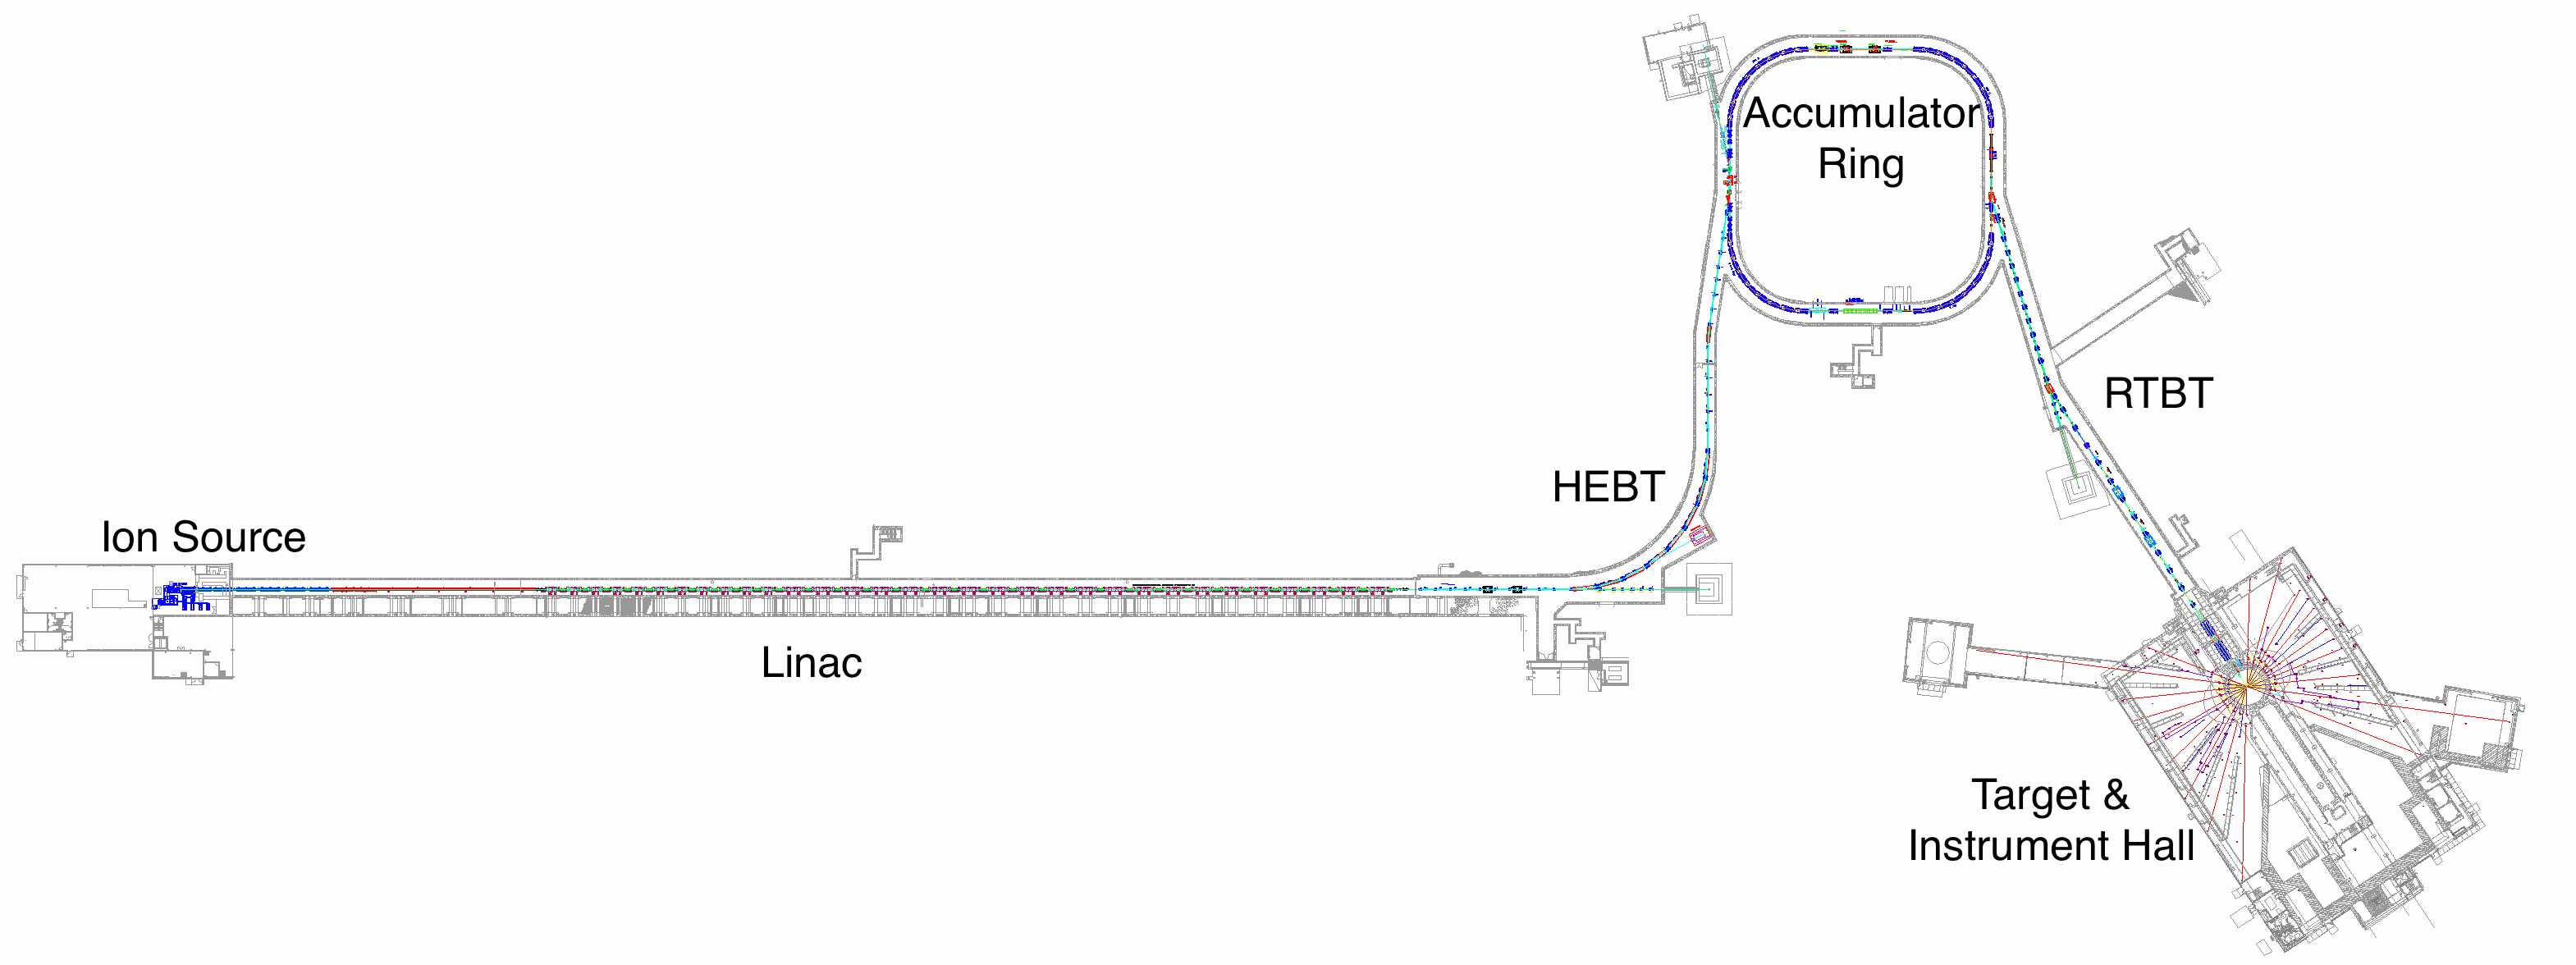
\includegraphics[angle=-90, width=0.5\textwidth]{Images/chapter1/SNS.png}
    \caption{Overview of the Spallation Neutron Source.}
    \label{fig:SNS}
\end{figure}
%

Fig.~\ref{fig:SNS_injection_region} zooms in on the injection region.
%
\begin{figure}[!p]
    \centering
    \begin{subfigure}{\textwidth}
        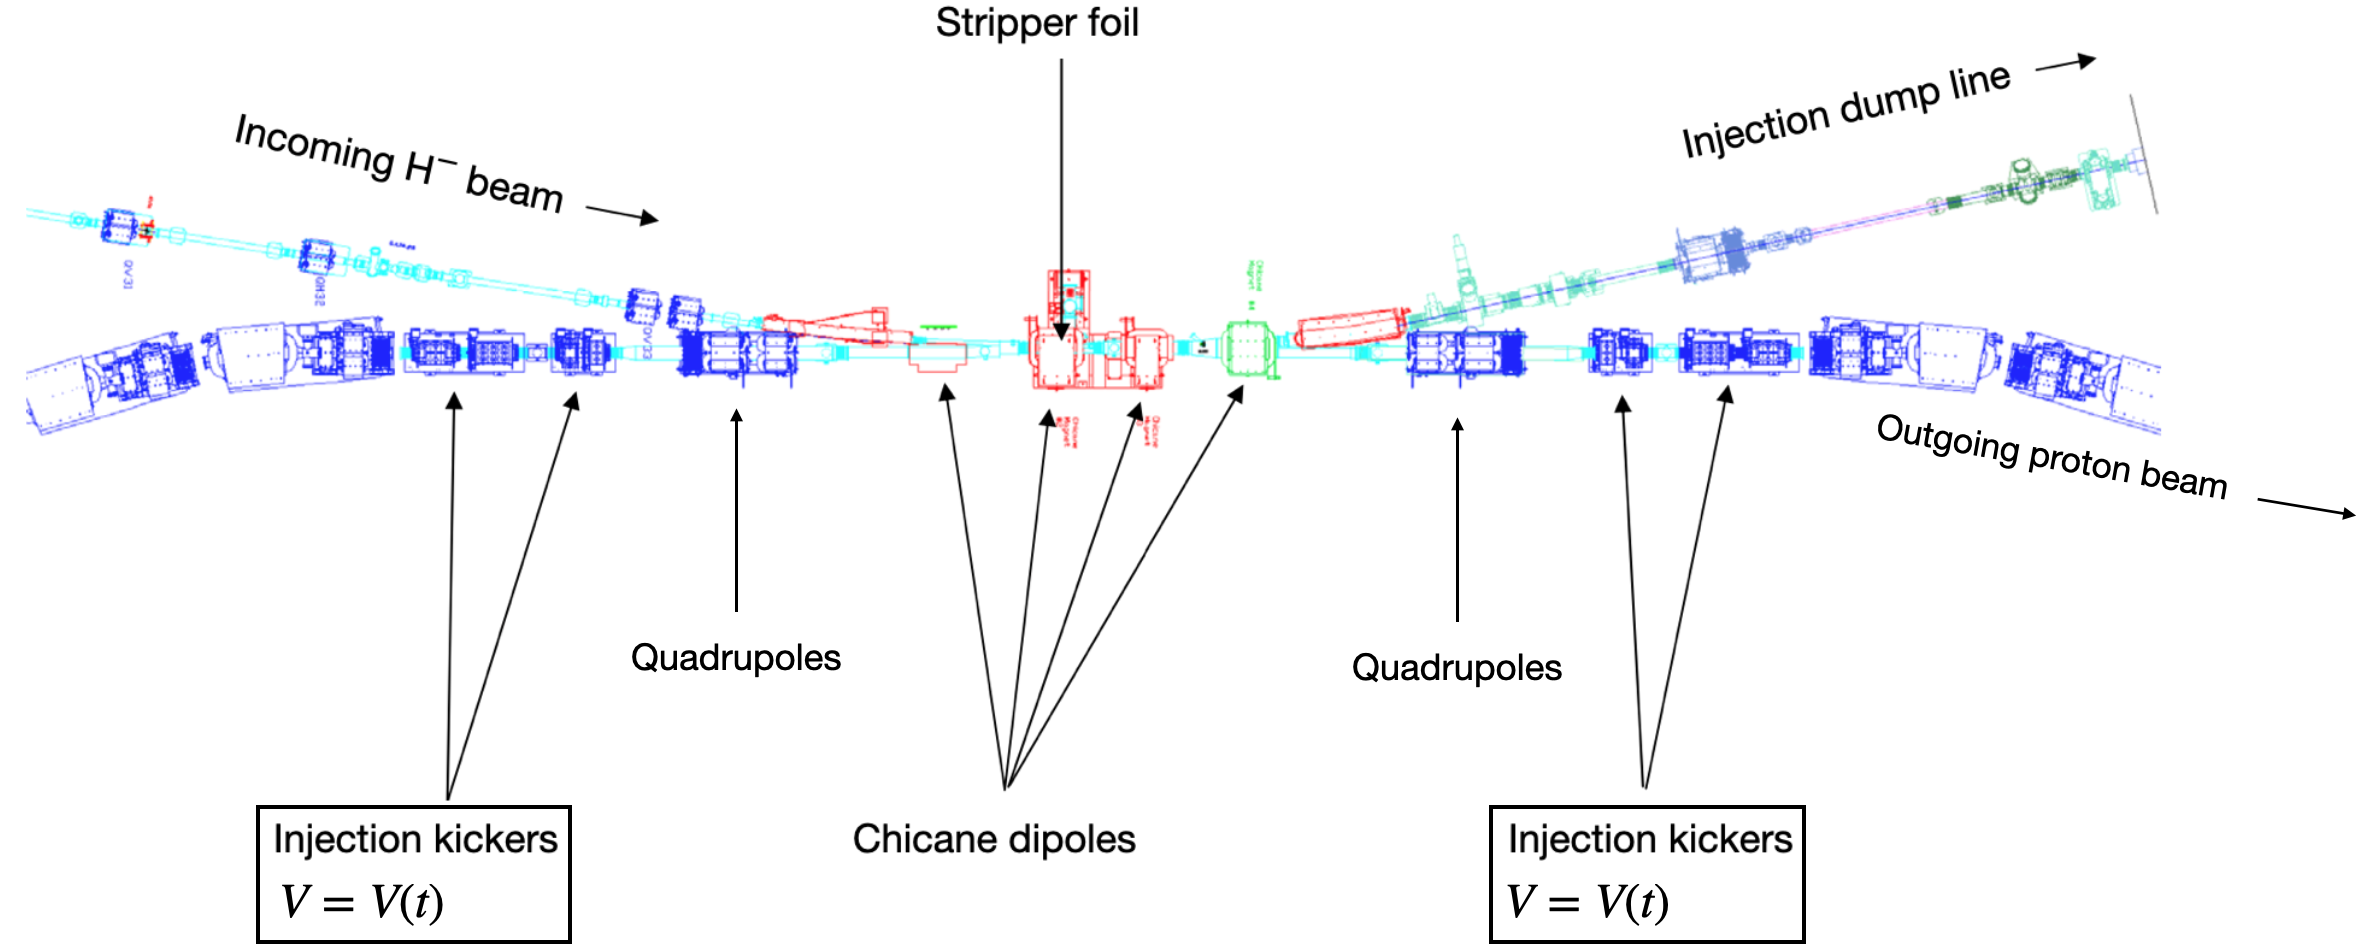
\includegraphics[width=\textwidth]{Images/chapter1/SNS_injection_region1.png}
        \label{fig:SNS_injection_region_a}
        \caption{}
    \end{subfigure}
    \vfill
    \vspace*{1.5cm}
    \vfill
    \begin{subfigure}{\textwidth}
        \centering
        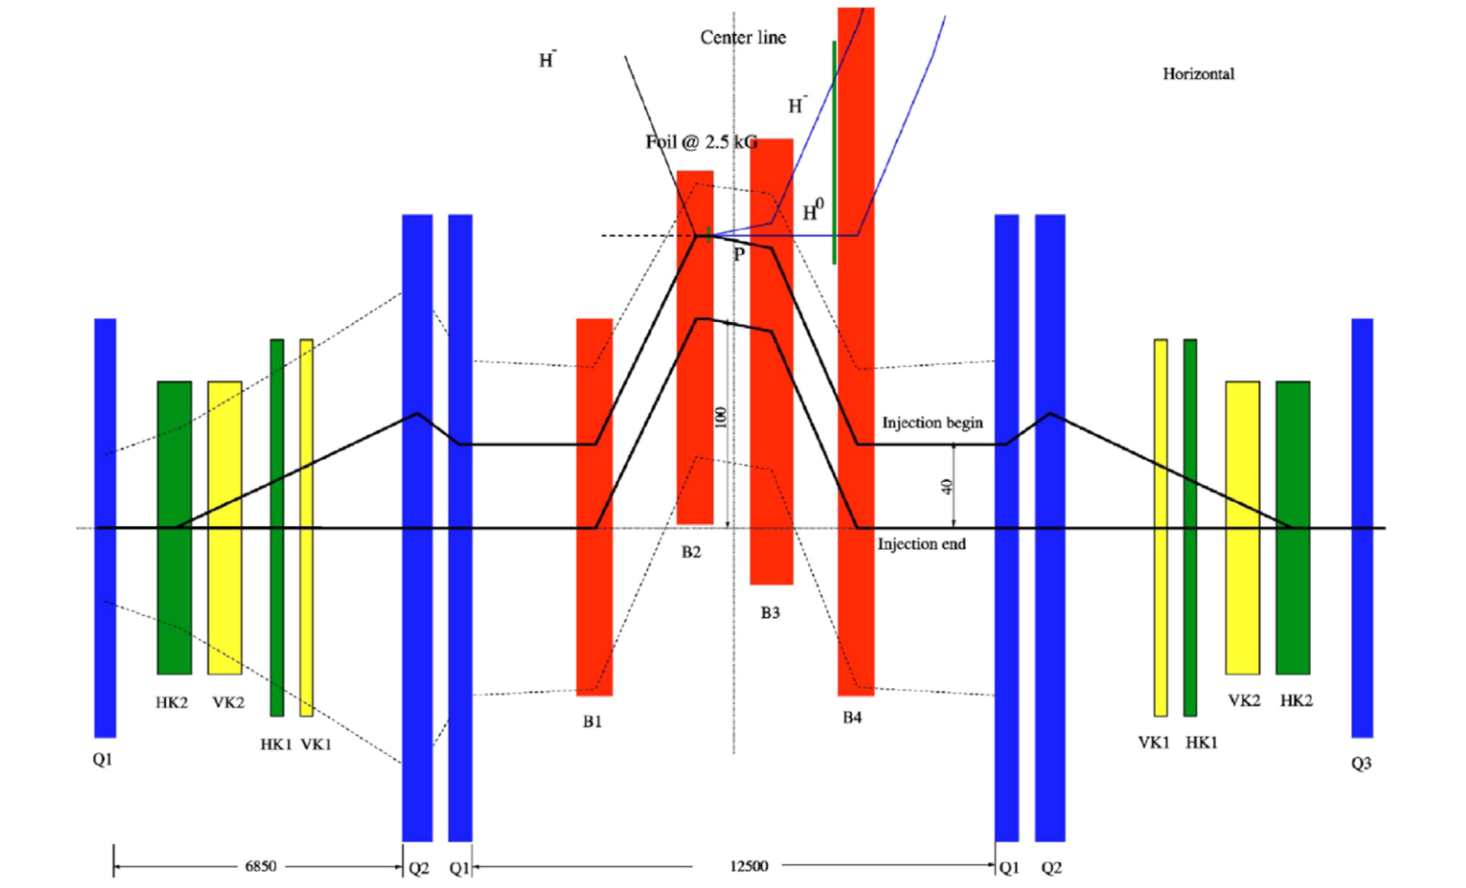
\includegraphics[width=\textwidth]{Images/chapter1/SNS_injection_region_2b.png}
        \caption{}
        \label{fig:SNS_injection_region_b}
    \end{subfigure}
    \caption{SNS injection region. (a) Overhead view of H$^-$ beam trajectory. (b) Schematic layout of the horizontal plane of the injection region: red = chicane dipoles, blue = quadrupoles, green = horizontal kickers, yellow = vertical kickers. (From \cite{Henderson2014}.)}
    \label{fig:SNS_injection_region}
\end{figure}
%
Four dipole magnets align the horizontal orbit with the beam from the linac at the foil. The injected beam trajectory is held fixed so that any remaining H$^0$ or H$^-$ particles can be reliably guided to a dump. Eight kicker magnets — four per plane — are available for time-dependent control of the position and slope of the orbit at the injection point. 


\subsubsection{Ring Injection Control application}

Each injection kicker magnet is given a waveform that scales the kicker voltage during injection. Once the initial and final voltages are known, they can be connected with a square root waveform to satisfy Eq.~\eqref{eq:elliptical_painting}. The time between the initial and final voltages (painting time) controls the final beam intensity. 

To control the position and angle of the orbit at the injection point, it is first necessary to measure the position and angle of the orbit at the injection point. This can be done indirectly as follows. A single minipulse is injected and stored in the ring, and its turn-by-turn mean transverse position is measured at one position using a beam-position-monitor (BPM). This is repeated for several minipulses and the average is taken. In the linear approximation, the mean position performs the pseudo-harmonic oscillations of Eq.~\eqref{eq:Hill_solution}; however, energy spread in the minipulse leads to decoherence — the mean position goes to zero. A Gaussian-damped sine wave is an accurate model of this process [\ref{}]:
%
\begin{equation}\label{eq:damped_sinusoid}
    x(t) = A_0 + A e^{kt^2} \cos{\left(\mu + \mu_0\right)},
\end{equation}
%
where $t$ is the turn number. The parameter $A$ gives the betatron amplitude, $\mu / 2\pi$ gives the fractional tune, and $\mu_0$ gives the particle phase at the BPM. The phase space coordinates recovered by combining these parameters with the linear ring model:
%
\begin{equation}
\begin{aligned}
    x_{bpm} &= A \cos\mu_0 \\ 
    x'_{bpm} &= -A\left({\sin\mu_0 + \frac{\alpha}{\beta}\cos\mu_0}\right).
\end{aligned}
\end{equation}
%
The coordinates are then transported to the injection point using the model transfer matrix. Repeating this for each BPM gives an estimated mean and standard deviation of the phase space coordinates at the injection point. Examples of measured individual and averaged BPM signals in the SNS ring are shown in Fig.~\ref{fig:bpm_avg} along with the damped-sinusoid fit. Additionally, a simulated minipulse in the (linearized) SNS ring is shown in Fig.~\ref{fig:minipulse}.
%
\begin{figure}[!p]
    \centering
    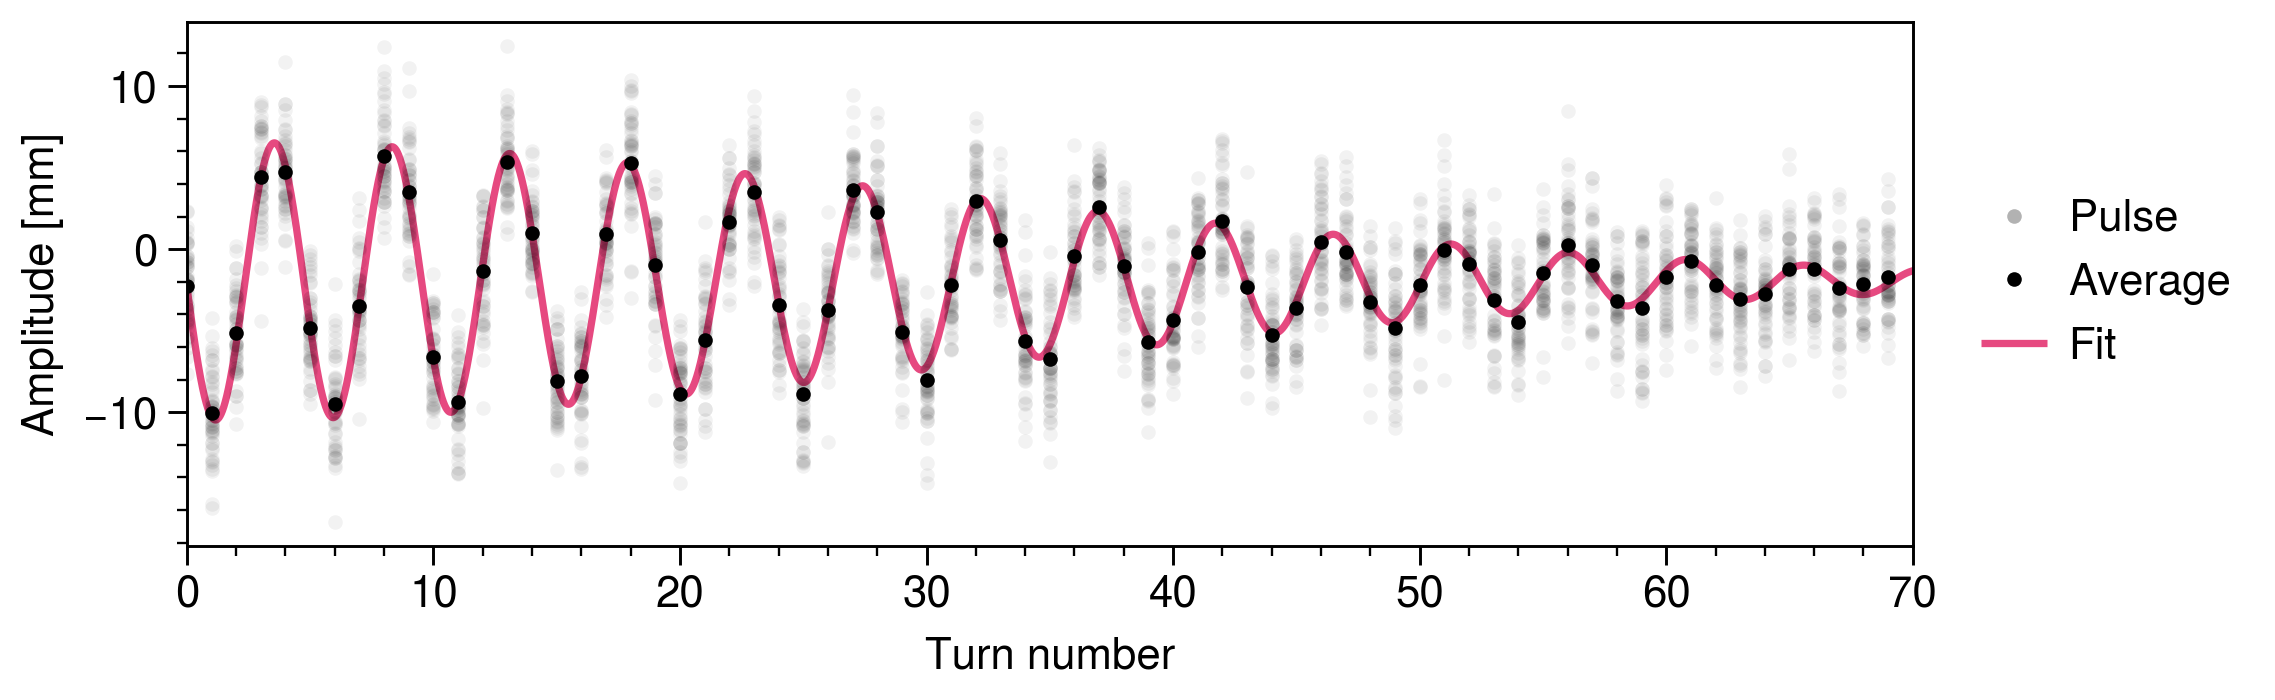
\includegraphics[width=\textwidth]{Images/chapter1/bpm_avg.png}
    \caption{Measured turn-by-turn BPM signal in the SNS ring — averaged over 50 pulses and fit with Eq.~\eqref{eq:damped_sinusoid}.}
    \label{fig:bpm_avg}
\end{figure}
%
%
\begin{figure}
    \centering
    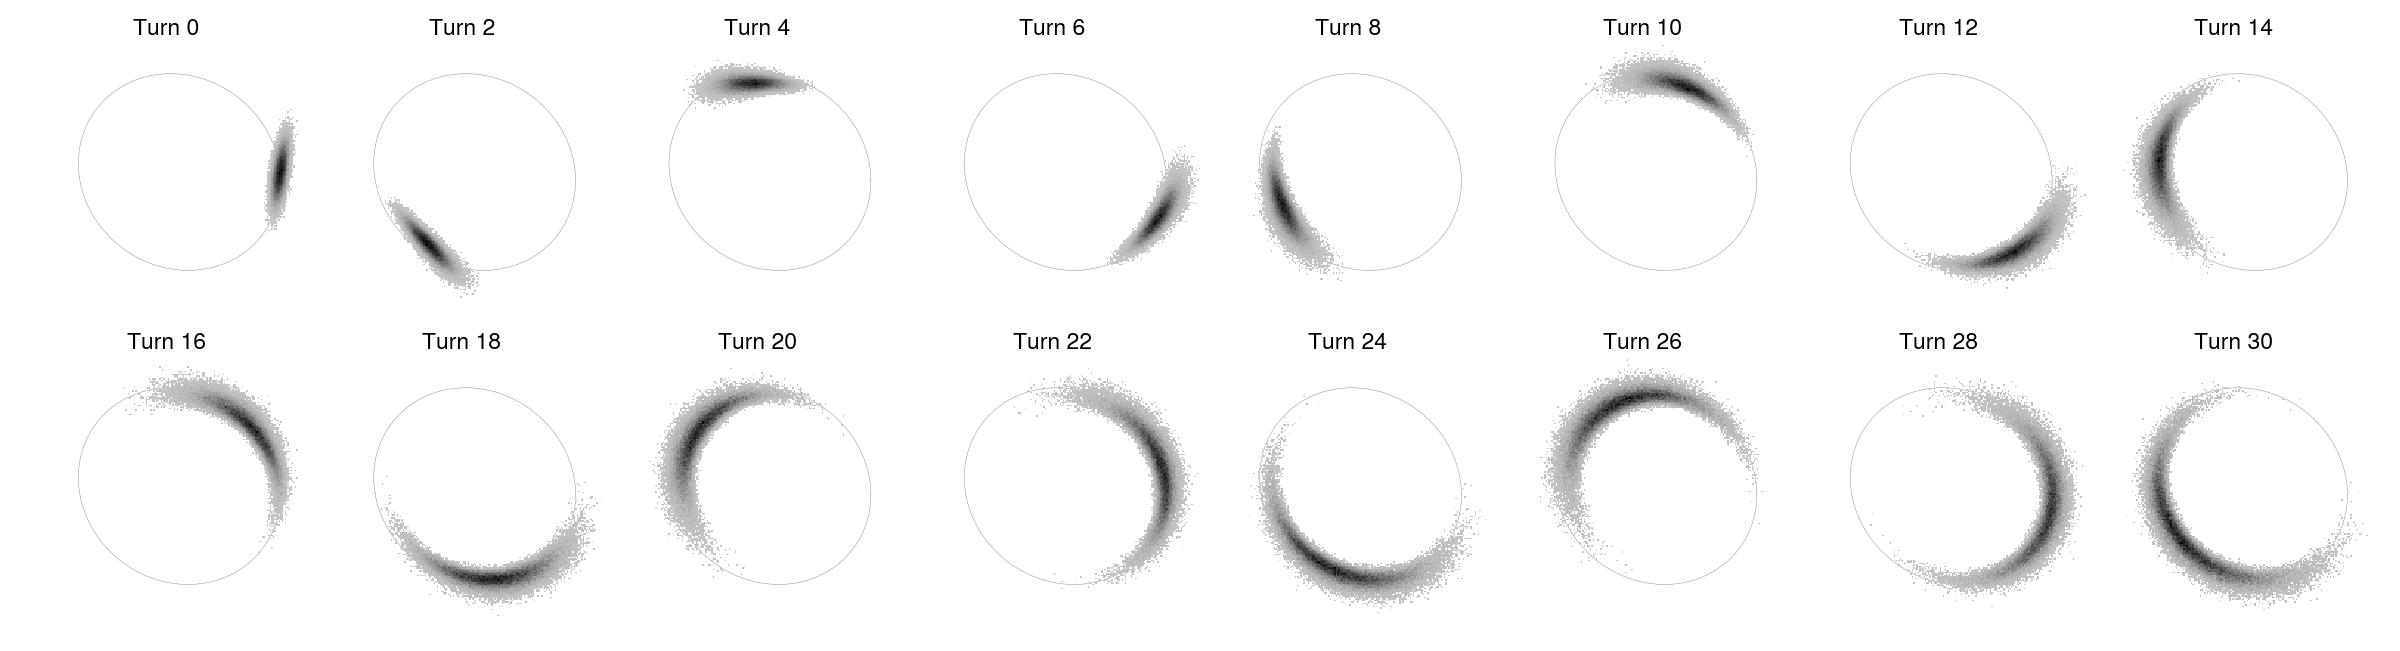
\includegraphics[width=\textwidth]{Images/chapter1/minipulse_chromaticity_black.png}
    \caption{Simulated minipulse in the (linearized) SNS ring. The $x$-$x'$ distribution is plotted at the injection point along with the Courant-Snyder ellipse.}
    \label{fig:minipulse}
\end{figure}
%

The next issue is how to control phase space coordinates at the injection point. Each kicker magnet is calibrated by applying a voltage difference to the magnet and measuring the orbit response using the ring BPMs; the angular kick associated with the magnet is varied until the model orbit agrees with the measured orbit. It was found that slight quadrupole corrections are necessary for this to occur. The standard deviation of the measured phase space coordinates is small after this calibration. One can then ask the model for a change in coordinates, update the kickers accordingly, and measure the new coordinates, iterating if necessary. This is currently done manually, and kicker power supplies need to be visually checked to make sure they are not beyond physical limits. Once this setup is complete, the kicker voltages are saved to a file and fed to a different script which scales sets the kicker waveforms. These steps were implemented as part of the Ring Injection Control (RIC) application in the OpenXAL framework \cite{Milas2021}. 

SNS injection kicker magnets have limited strengths and are unipolar, which limits the minimum distance between the ring orbit and the foil as well as the maximum angle at the injection point. In fact, the closed orbit cannot reach the foil at production energy (1 GeV). As will be discussed later, the beam energy can be lowered to increase the effective kicker strength; however, this is a significant task for SNS operators due to issues related to the SNS timing system. Initial attempts to lower the energy to 0.6 GeV were unsuccessful, but an energy of 0.8 GeV was recently achieved. 



\section{Goals of this dissertation}\label{sec:Goals of this dissertation}.

The goal of this dissertation is to contribute to efforts to generate a Danilov distribution in the SNS ring. An additional goal is to improve the current understanding of the dynamics of the Danilov distribution with space charge.

In chapter \ref{chap-2}, envelope equations describing the linear transport of the Danilov distribution are studied. In particular, insight is gained by computing the matched beam envelope in the presence of space charge and linear external coupling. In chapter \ref{chap-3}, particle-in-cell (PIC) simulations of elliptical painting in the SNS are carried out, building on previous work. In chapter \ref{chap-4}, methods are proposed to measure the similarity between a painted distribution in the SNS ring and a Danilov distribution. The methods are simulated and implemented in the SNS. In chapter \ref{chap-5}, elliptical painting is carried out in the SNS for the first time; measurements compared with simulation. Finally, implications and extensions of this work are discussed in chapter \ref{chap-6}.
